\documentclass[twoside]{article}

% Packages required by doxygen
\usepackage{fixltx2e}
\usepackage{calc}
\usepackage{doxygen}
\usepackage[export]{adjustbox} % also loads graphicx
\usepackage{graphicx}
\usepackage[utf8]{inputenc}
\usepackage{makeidx}
\usepackage{multicol}
\usepackage{multirow}
\PassOptionsToPackage{warn}{textcomp}
\usepackage{textcomp}
\usepackage[nointegrals]{wasysym}
\usepackage[table]{xcolor}

% NLS support packages
\usepackage[danish]{babel}
\usepackage[T1]{fontenc}

% Font selection
\usepackage[T1]{fontenc}
\usepackage[scaled=.90]{helvet}
\usepackage{courier}
\usepackage{amssymb}
\usepackage{sectsty}
\renewcommand{\familydefault}{\sfdefault}
\allsectionsfont{%
  \fontseries{bc}\selectfont%
  \color{darkgray}%
}
\renewcommand{\DoxyLabelFont}{%
  \fontseries{bc}\selectfont%
  \color{darkgray}%
}
\newcommand{\+}{\discretionary{\mbox{\scriptsize$\hookleftarrow$}}{}{}}

% Page & text layout
\usepackage{geometry}
\geometry{%
  a4paper,%
  top=2.5cm,%
  bottom=2.5cm,%
  left=2.5cm,%
  right=2.5cm%
}
\tolerance=750
\hfuzz=15pt
\hbadness=750
\setlength{\emergencystretch}{15pt}
\setlength{\parindent}{0cm}
\setlength{\parskip}{3ex plus 2ex minus 2ex}
\makeatletter
\renewcommand{\paragraph}{%
  \@startsection{paragraph}{4}{0ex}{-1.0ex}{1.0ex}{%
    \normalfont\normalsize\bfseries\SS@parafont%
  }%
}
\renewcommand{\subparagraph}{%
  \@startsection{subparagraph}{5}{0ex}{-1.0ex}{1.0ex}{%
    \normalfont\normalsize\bfseries\SS@subparafont%
  }%
}
\makeatother

% Headers & footers
\usepackage{fancyhdr}
\pagestyle{fancyplain}
\fancyhead[LE]{\fancyplain{}{\bfseries\thepage}}
\fancyhead[CE]{\fancyplain{}{}}
\fancyhead[RE]{\fancyplain{}{\bfseries\leftmark}}
\fancyhead[LO]{\fancyplain{}{\bfseries\rightmark}}
\fancyhead[CO]{\fancyplain{}{}}
\fancyhead[RO]{\fancyplain{}{\bfseries\thepage}}
\fancyfoot[LE]{\fancyplain{}{}}
\fancyfoot[CE]{\fancyplain{}{}}
\fancyfoot[RE]{\fancyplain{}{\bfseries\scriptsize Genereret af Doxygen }}
\fancyfoot[LO]{\fancyplain{}{\bfseries\scriptsize Genereret af Doxygen }}
\fancyfoot[CO]{\fancyplain{}{}}
\fancyfoot[RO]{\fancyplain{}{}}
\renewcommand{\footrulewidth}{0.4pt}
\renewcommand{\sectionmark}[1]{%
  \markright{\thesection\ #1}%
}

% Indices & bibliography
\usepackage{natbib}
\usepackage[titles]{tocloft}
\setcounter{tocdepth}{3}
\setcounter{secnumdepth}{5}
\makeindex

% Hyperlinks (required, but should be loaded last)
\usepackage{ifpdf}
\ifpdf
  \usepackage[pdftex,pagebackref=true]{hyperref}
\else
  \usepackage[ps2pdf,pagebackref=true]{hyperref}
\fi
\hypersetup{%
  colorlinks=true,%
  linkcolor=blue,%
  citecolor=blue,%
  unicode%
}

% Custom commands
\newcommand{\clearemptydoublepage}{%
  \newpage{\pagestyle{empty}\cleardoublepage}%
}

\usepackage{caption}
\captionsetup{labelsep=space,justification=centering,font={bf},singlelinecheck=off,skip=4pt,position=top}

%===== C O N T E N T S =====

\begin{document}

% Titlepage & ToC
\hypersetup{pageanchor=false,
             bookmarksnumbered=true,
             pdfencoding=unicode
            }
\pagenumbering{roman}
\begin{titlepage}
\vspace*{7cm}
\begin{center}%
{\Large L.\+A.\+M.\+P -\/ P\+SoC Z }\\
\vspace*{1cm}
{\large Genereret af Doxygen 1.8.11}\\
\end{center}
\end{titlepage}
\tableofcontents
\pagenumbering{arabic}
\hypersetup{pageanchor=true}

%--- Begin generated contents ---
\section{Indeks over datastrukturer}
\subsection{Datastrukturer}
Her er datastrukturerne med korte beskrivelser\+:\begin{DoxyCompactList}
\item\contentsline{section}{\hyperlink{class_e3_p_j_r}{E3\+P\+JR} }{\pageref{class_e3_p_j_r}}{}
\item\contentsline{section}{\hyperlink{class_ui_1_1_e3_p_j_r}{E3\+P\+JR} }{\pageref{class_ui_1_1_e3_p_j_r}}{}
\item\contentsline{section}{\hyperlink{class_light}{Light} }{\pageref{class_light}}{}
\item\contentsline{section}{\hyperlink{class_main_display}{Main\+Display} }{\pageref{class_main_display}}{}
\item\contentsline{section}{\hyperlink{class_planner}{Planner} }{\pageref{class_planner}}{}
\item\contentsline{section}{\hyperlink{class_planner_dialog}{Planner\+Dialog} }{\pageref{class_planner_dialog}}{}
\item\contentsline{section}{\hyperlink{class_q_dialog}{Q\+Dialog} }{\pageref{class_q_dialog}}{}
\item\contentsline{section}{\hyperlink{class_q_tab_widget}{Q\+Tab\+Widget} }{\pageref{class_q_tab_widget}}{}
\item\contentsline{section}{\hyperlink{class_q_virtual_keyboard}{Q\+Virtual\+Keyboard} }{\pageref{class_q_virtual_keyboard}}{}
\item\contentsline{section}{\hyperlink{class_q_widget}{Q\+Widget} }{\pageref{class_q_widget}}{}
\item\contentsline{section}{\hyperlink{class_s_p_iapi}{S\+P\+Iapi} }{\pageref{class_s_p_iapi}}{}
\item\contentsline{section}{\hyperlink{class_spi_test_program}{Spi\+Test\+Program} }{\pageref{class_spi_test_program}}{}
\item\contentsline{section}{\hyperlink{class_ui_1_1_spi_test_program}{Spi\+Test\+Program} }{\pageref{class_ui_1_1_spi_test_program}}{}
\item\contentsline{section}{\hyperlink{class_ui___e3_p_j_r}{Ui\+\_\+\+E3\+P\+JR} }{\pageref{class_ui___e3_p_j_r}}{}
\item\contentsline{section}{\hyperlink{class_ui___spi_test_program}{Ui\+\_\+\+Spi\+Test\+Program} }{\pageref{class_ui___spi_test_program}}{}
\end{DoxyCompactList}

\section{Fil-\/indeks}
\subsection{Filoversigt}
Her er en liste over alle filer med korte beskrivelser\+:\begin{DoxyCompactList}
\item\contentsline{section}{\hyperlink{cyapicallbacks_8h}{cyapicallbacks.\+h} }{\pageref{cyapicallbacks_8h}}{}
\item\contentsline{section}{\hyperlink{data_8c}{data.\+c} \\*\hyperlink{class_data}{Data} modul }{\pageref{data_8c}}{}
\item\contentsline{section}{\hyperlink{data_8h}{data.\+h} \\*\hyperlink{class_data}{Data} modul }{\pageref{data_8h}}{}
\item\contentsline{section}{\hyperlink{handler_8c}{handler.\+c} \\*\hyperlink{class_handler}{Handler} modul }{\pageref{handler_8c}}{}
\item\contentsline{section}{\hyperlink{handler_8h}{handler.\+h} \\*\hyperlink{class_handler}{Handler} modul }{\pageref{handler_8h}}{}
\item\contentsline{section}{\hyperlink{i2c_8c}{i2c.\+c} \\*\hyperlink{class_i2_c}{I2C} modul }{\pageref{i2c_8c}}{}
\item\contentsline{section}{\hyperlink{i2c_8h}{i2c.\+h} \\*\hyperlink{class_i2_c}{I2C} modul }{\pageref{i2c_8h}}{}
\item\contentsline{section}{\hyperlink{lcd_8c}{lcd.\+c} \\*\hyperlink{class_l_c_d}{L\+CD} modul }{\pageref{lcd_8c}}{}
\item\contentsline{section}{\hyperlink{lcd_8h}{lcd.\+h} \\*\hyperlink{class_l_c_d}{L\+CD} modul }{\pageref{lcd_8h}}{}
\item\contentsline{section}{\hyperlink{led_8c}{led.\+c} \\*\hyperlink{class_l_e_d}{L\+ED} modul }{\pageref{led_8c}}{}
\item\contentsline{section}{\hyperlink{led_8h}{led.\+h} \\*\hyperlink{class_l_e_d}{L\+ED} modul }{\pageref{led_8h}}{}
\item\contentsline{section}{\hyperlink{main_8c}{main.\+c} \\*Hovedprogram }{\pageref{main_8c}}{}
\item\contentsline{section}{\hyperlink{queue_8c}{queue.\+c} \\*\hyperlink{class_queue}{Queue} modul }{\pageref{queue_8c}}{}
\item\contentsline{section}{\hyperlink{queue_8h}{queue.\+h} \\*\hyperlink{class_queue}{Queue} modul }{\pageref{queue_8h}}{}
\item\contentsline{section}{\hyperlink{spi_8c}{spi.\+c} \\*\hyperlink{class_s_p_i}{S\+PI} modul }{\pageref{spi_8c}}{}
\item\contentsline{section}{\hyperlink{spi_8h}{spi.\+h} \\*\hyperlink{class_s_p_i}{S\+PI} modul }{\pageref{spi_8h}}{}
\end{DoxyCompactList}

\section{Datastruktur-\/documentation}
\hypertarget{class_data}{}\subsection{Data Klasse-\/reference}
\label{class_data}\index{Data@{Data}}


\hyperlink{class_data}{Data} class.  




{\ttfamily \#include $<$data.\+h$>$}



Samarbejdsdiagram for Data\+:\nopagebreak
\begin{figure}[H]
\begin{center}
\leavevmode
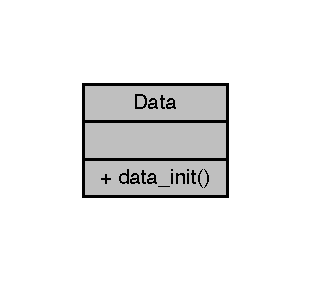
\includegraphics[width=149pt]{class_data__coll__graph}
\end{center}
\end{figure}
\subsubsection*{Offentlige metoder}
\begin{DoxyCompactItemize}
\item 
void \hyperlink{class_data_a68c6d4c829f9363c7d9ff2efbbca50c1}{data\+\_\+init} ()
\begin{DoxyCompactList}\small\item\em Initialiser data modulet. \end{DoxyCompactList}\end{DoxyCompactItemize}


\subsubsection{Detaljeret beskrivelse}
\hyperlink{class_data}{Data} class. 

Indeholder data hentet fra P\+So\+C-\/\+XY, -\/Z og -\/\+Sensor. \begin{DoxyAuthor}{Forfatter}
Jeppe Stærk Antonsen (\href{mailto:201271201@uni.au.dk}{\tt 201271201@uni.\+au.\+dk}) 
\end{DoxyAuthor}


\subsubsection{Dokumentation af medlemsfunktioner}
\index{Data@{Data}!data\+\_\+init@{data\+\_\+init}}
\index{data\+\_\+init@{data\+\_\+init}!Data@{Data}}
\paragraph[{\texorpdfstring{data\+\_\+init()}{data_init()}}]{\setlength{\rightskip}{0pt plus 5cm}void data\+\_\+init (
\begin{DoxyParamCaption}
\item[{void}]{}
\end{DoxyParamCaption}
)}\hypertarget{class_data_a68c6d4c829f9363c7d9ff2efbbca50c1}{}\label{class_data_a68c6d4c829f9363c7d9ff2efbbca50c1}


Initialiser data modulet. 

Initialiser data structen med 0 værdier.

\begin{DoxyAuthor}{Forfatter}
Jeppe Stærk Antonsen (\href{mailto:201271201@uni.au.dk}{\tt 201271201@uni.\+au.\+dk}) 
\end{DoxyAuthor}


Defineret på linje 20 i filen data.\+c.



Indeholder referencer til Data\+Master\+::b\+Val, data\+Master, Data\+Master\+::g\+Val, Data\+Master\+::r\+Val, Data\+Master\+::x\+Val, Data\+Master\+::y\+Val og Data\+Master\+::z\+Val.



Refereret til af main().


\begin{DoxyCode}
21 \{
22   \hyperlink{data_8h_a6b1a8871e30b304a6f5764c44d89e489}{dataMaster}.\hyperlink{data_8h_a7849f509240fa25127fcda8c5009f02b}{xVal} = 0;
23   \hyperlink{data_8h_a6b1a8871e30b304a6f5764c44d89e489}{dataMaster}.\hyperlink{data_8h_a28e89368b5a1aee30ccd952ad63e8c55}{yVal} = 0;
24   \hyperlink{data_8h_a6b1a8871e30b304a6f5764c44d89e489}{dataMaster}.\hyperlink{data_8h_a767a084c35fdc0f1e3e41972d5415483}{zVal} = 0;
25   \hyperlink{data_8h_a6b1a8871e30b304a6f5764c44d89e489}{dataMaster}.\hyperlink{data_8h_a3bf14030a39e71a91c0b97a624f95c5d}{rVal} = 0;
26   \hyperlink{data_8h_a6b1a8871e30b304a6f5764c44d89e489}{dataMaster}.\hyperlink{data_8h_ae02d0c792549f1b88e80ae6eb117f2be}{gVal} = 0;
27   \hyperlink{data_8h_a6b1a8871e30b304a6f5764c44d89e489}{dataMaster}.\hyperlink{data_8h_adf9e1f80891d4eaa914c2bde2502cdf2}{bVal} = 0;
28 \}
\end{DoxyCode}


Her er kalder-\/grafen for denne funktion\+:\nopagebreak
\begin{figure}[H]
\begin{center}
\leavevmode
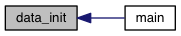
\includegraphics[width=207pt]{class_data_a68c6d4c829f9363c7d9ff2efbbca50c1_icgraph}
\end{center}
\end{figure}




Dokumentationen for denne klasse blev genereret ud fra filerne\+:\begin{DoxyCompactItemize}
\item 
\hyperlink{data_8h}{data.\+h}\item 
\hyperlink{data_8c}{data.\+c}\end{DoxyCompactItemize}

\hypertarget{class_handler}{}\subsection{Handler Klasse-\/reference}
\label{class_handler}\index{Handler@{Handler}}


\hyperlink{class_handler}{Handler} class.  




{\ttfamily \#include $<$handler.\+h$>$}



Samarbejdsdiagram for Handler\+:
\nopagebreak
\begin{figure}[H]
\begin{center}
\leavevmode
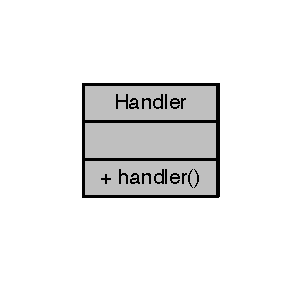
\includegraphics[width=145pt]{d9/de1/class_handler__coll__graph}
\end{center}
\end{figure}
\subsubsection*{Offentlige metoder}
\begin{DoxyCompactItemize}
\item 
void \hyperlink{class_handler_af5be5b016b862943cd22504490acc8f4}{handler} (uint8 cmd, uint8 val)
\begin{DoxyCompactList}\small\item\em Håndter kommando med tilhørende værdi. \end{DoxyCompactList}\end{DoxyCompactItemize}


\subsubsection{Detaljeret beskrivelse}
\hyperlink{class_handler}{Handler} class. 

Håndtere indkommende kommandoer med tilhørende værdier. \begin{DoxyAuthor}{Forfatter}
Jeppe Stærk Antonsen (\href{mailto:201271201@uni.au.dk}{\tt 201271201@uni.\+au.\+dk}) 
\end{DoxyAuthor}


\subsubsection{Dokumentation af medlemsfunktioner}
\index{Handler@{Handler}!handler@{handler}}
\index{handler@{handler}!Handler@{Handler}}
\paragraph[{\texorpdfstring{handler(uint8 cmd, uint8 val)}{handler(uint8 cmd, uint8 val)}}]{\setlength{\rightskip}{0pt plus 5cm}void handler (
\begin{DoxyParamCaption}
\item[{uint8}]{cmd, }
\item[{uint8}]{val}
\end{DoxyParamCaption}
)}\hypertarget{class_handler_af5be5b016b862943cd22504490acc8f4}{}\label{class_handler_af5be5b016b862943cd22504490acc8f4}


Håndter kommando med tilhørende værdi. 

Fortager en defineret handling ud fra den modtaget kommando med den tilhørende værdi. 
\begin{DoxyParams}[1]{Parametre}
\mbox{\tt in}  & {\em cmd} & Er den modtaget kommando. \\
\hline
\mbox{\tt in}  & {\em val} & Er den tilhørende værdi.\\
\hline
\end{DoxyParams}
\begin{DoxyAuthor}{Forfatter}
Jeppe Stærk Antonsen (\href{mailto:201271201@uni.au.dk}{\tt 201271201@uni.\+au.\+dk}) 
\end{DoxyAuthor}


Defineret på linje 26 i filen handler.\+c.



Indeholder referencer til Data\+Master\+::b\+Val, C\+M\+D\+\_\+\+D\+I\+S\+T\+A\+N\+C\+E\+\_\+\+A\+L\+RT, C\+M\+D\+\_\+\+G\+E\+T\+\_\+\+B\+L\+U\+E\+\_\+\+V\+AL, C\+M\+D\+\_\+\+G\+E\+T\+\_\+\+D\+I\+S\+T\+A\+N\+C\+E\+\_\+\+S\+TS, C\+M\+D\+\_\+\+G\+E\+T\+\_\+\+G\+R\+E\+E\+N\+\_\+\+V\+AL, C\+M\+D\+\_\+\+G\+E\+T\+\_\+\+L\+U\+M\+E\+N\+\_\+\+V\+AL, C\+M\+D\+\_\+\+G\+E\+T\+\_\+\+M\+O\+V\+E\+M\+E\+N\+T\+\_\+\+S\+TS, C\+M\+D\+\_\+\+G\+E\+T\+\_\+\+P\+O\+W\+E\+R\+\_\+\+S\+TS, C\+M\+D\+\_\+\+G\+E\+T\+\_\+\+R\+E\+D\+\_\+\+V\+AL, C\+M\+D\+\_\+\+G\+E\+T\+\_\+\+X\+\_\+\+P\+OS, C\+M\+D\+\_\+\+G\+E\+T\+\_\+\+Y\+\_\+\+P\+OS, C\+M\+D\+\_\+\+G\+E\+T\+\_\+\+Z\+\_\+\+P\+OS, C\+M\+D\+\_\+\+M\+O\+V\+E\+M\+E\+N\+T\+\_\+\+A\+L\+RT, C\+M\+D\+\_\+\+S\+E\+T\+\_\+\+B\+L\+U\+E\+\_\+\+V\+AL, C\+M\+D\+\_\+\+S\+E\+T\+\_\+\+D\+I\+S\+T\+A\+N\+C\+E\+\_\+\+S\+TS, C\+M\+D\+\_\+\+S\+E\+T\+\_\+\+G\+R\+E\+E\+N\+\_\+\+V\+AL, C\+M\+D\+\_\+\+S\+E\+T\+\_\+\+L\+U\+M\+E\+N\+\_\+\+V\+AL, C\+M\+D\+\_\+\+S\+E\+T\+\_\+\+M\+O\+V\+E\+M\+E\+N\+T\+\_\+\+S\+TS, C\+M\+D\+\_\+\+S\+E\+T\+\_\+\+P\+O\+W\+E\+R\+\_\+\+S\+TS, C\+M\+D\+\_\+\+S\+E\+T\+\_\+\+R\+E\+D\+\_\+\+V\+AL, C\+M\+D\+\_\+\+S\+E\+T\+\_\+\+X\+\_\+\+P\+OS, C\+M\+D\+\_\+\+S\+E\+T\+\_\+\+Y\+\_\+\+P\+OS, C\+M\+D\+\_\+\+S\+E\+T\+\_\+\+Z\+\_\+\+P\+OS, C\+M\+D\+\_\+\+X\+\_\+\+C\+AL, C\+M\+D\+\_\+\+X\+\_\+\+S\+TP, C\+M\+D\+\_\+\+Y\+\_\+\+C\+AL, C\+M\+D\+\_\+\+Y\+\_\+\+S\+TP, C\+M\+D\+\_\+\+Z\+\_\+\+C\+AL, C\+M\+D\+\_\+\+Z\+\_\+\+S\+TP, data\+Master, Data\+Master\+::g\+Val, I2\+C\+::i2c\+\_\+get\+Packet(), I2\+C\+::i2c\+\_\+set\+Packet(), P\+So\+C\+\_\+\+Sensor, P\+So\+C\+\_\+\+XY, P\+So\+C\+\_\+Z, Data\+Master\+::r\+Val, Data\+Master\+::x\+Val, Data\+Master\+::y\+Val og Data\+Master\+::z\+Val.



Refereret til af main().


\begin{DoxyCode}
27 \{
28   DEBUG\_PutString(\textcolor{stringliteral}{"H=: cmd: "});
29   DEBUG\_PutHexByte(\hyperlink{queue_8h_a85092d82ab6ea85dad51ba78cbda36a0}{cmd});
30   DEBUG\_PutString(\textcolor{stringliteral}{" val: "});
31   DEBUG\_PutHexByte(\hyperlink{queue_8h_aa0ccb5ee6d882ee3605ff47745c6467b}{val});
32   DEBUG\_PutCRLF();
33   
34   \textcolor{keywordflow}{switch} (\hyperlink{queue_8h_a85092d82ab6ea85dad51ba78cbda36a0}{cmd})
35   \{
36     \textcolor{keywordflow}{case} 0x01 :
37       \hyperlink{i2c_8h_afd44ef28b428b7ec2cffb38c97340251}{i2c\_getPacket}(\hyperlink{i2c_8h_a2c70db7df8defae29c1912d84aaee3dc}{PSoC\_XY}, \hyperlink{handler_8h_aa50e083669624eeaef782ebc867008f9}{CMD\_GET\_X\_POS}, &
      \hyperlink{data_8h_a6b1a8871e30b304a6f5764c44d89e489}{dataMaster}.\hyperlink{data_8h_a7849f509240fa25127fcda8c5009f02b}{xVal});
38       \hyperlink{i2c_8h_afd44ef28b428b7ec2cffb38c97340251}{i2c\_getPacket}(\hyperlink{i2c_8h_a2c70db7df8defae29c1912d84aaee3dc}{PSoC\_XY}, \hyperlink{handler_8h_a51053e5251048d6ebbf4d2e23de40761}{CMD\_GET\_Y\_POS}, &
      \hyperlink{data_8h_a6b1a8871e30b304a6f5764c44d89e489}{dataMaster}.\hyperlink{data_8h_a28e89368b5a1aee30ccd952ad63e8c55}{yVal});
39       \hyperlink{i2c_8h_afd44ef28b428b7ec2cffb38c97340251}{i2c\_getPacket}(\hyperlink{i2c_8h_aa72315d85eb390444fdd96475c6aa1f4}{PSoC\_Z}, \hyperlink{handler_8h_a4d76e78d09a00f75609569d9aa92ab98}{CMD\_GET\_Z\_POS}, &
      \hyperlink{data_8h_a6b1a8871e30b304a6f5764c44d89e489}{dataMaster}.\hyperlink{data_8h_a767a084c35fdc0f1e3e41972d5415483}{zVal});
40       \textcolor{keywordflow}{break};
41     \textcolor{keywordflow}{case} 0x03 :
42       \hyperlink{i2c_8h_afd44ef28b428b7ec2cffb38c97340251}{i2c\_getPacket}(\hyperlink{i2c_8h_adc44ca05813864518773ea6f3543816c}{PSoC\_Sensor}, \hyperlink{handler_8h_aa2f09e60c4eeae4560da88c6b1b08c60}{CMD\_GET\_RED\_VAL}, &
      \hyperlink{data_8h_a6b1a8871e30b304a6f5764c44d89e489}{dataMaster}.\hyperlink{data_8h_a3bf14030a39e71a91c0b97a624f95c5d}{rVal});
43       \hyperlink{i2c_8h_afd44ef28b428b7ec2cffb38c97340251}{i2c\_getPacket}(\hyperlink{i2c_8h_adc44ca05813864518773ea6f3543816c}{PSoC\_Sensor}, \hyperlink{handler_8h_a81052c67f996705d7eacfcea66bdde08}{CMD\_GET\_BLUE\_VAL}, &
      \hyperlink{data_8h_a6b1a8871e30b304a6f5764c44d89e489}{dataMaster}.\hyperlink{data_8h_ae02d0c792549f1b88e80ae6eb117f2be}{gVal});
44       \hyperlink{i2c_8h_afd44ef28b428b7ec2cffb38c97340251}{i2c\_getPacket}(\hyperlink{i2c_8h_adc44ca05813864518773ea6f3543816c}{PSoC\_Sensor}, \hyperlink{handler_8h_a55d24f50aeb52afddd491d97a66c81ef}{CMD\_GET\_GREEN\_VAL}, &
      \hyperlink{data_8h_a6b1a8871e30b304a6f5764c44d89e489}{dataMaster}.\hyperlink{data_8h_adf9e1f80891d4eaa914c2bde2502cdf2}{bVal});
45       \textcolor{keywordflow}{break};
46     \textcolor{keywordflow}{case} \hyperlink{handler_8h_af70b73890a98cfe329a916df037f46a4}{CMD\_SET\_X\_POS} :
47       \hyperlink{i2c_8h_a0e13c9c7d87ebdb3680495a787f68d29}{i2c\_setPacket}(\hyperlink{i2c_8h_a2c70db7df8defae29c1912d84aaee3dc}{PSoC\_XY}, \hyperlink{queue_8h_a85092d82ab6ea85dad51ba78cbda36a0}{cmd}, \hyperlink{queue_8h_aa0ccb5ee6d882ee3605ff47745c6467b}{val});
48       \textcolor{keywordflow}{break};
49     \textcolor{keywordflow}{case} \hyperlink{handler_8h_a82640a671f668fb40ff4851901d5a151}{CMD\_SET\_Y\_POS} :
50       \hyperlink{i2c_8h_a0e13c9c7d87ebdb3680495a787f68d29}{i2c\_setPacket}(\hyperlink{i2c_8h_a2c70db7df8defae29c1912d84aaee3dc}{PSoC\_XY}, \hyperlink{queue_8h_a85092d82ab6ea85dad51ba78cbda36a0}{cmd}, \hyperlink{queue_8h_aa0ccb5ee6d882ee3605ff47745c6467b}{val});
51       \textcolor{keywordflow}{break};
52     \textcolor{keywordflow}{case} \hyperlink{handler_8h_aa50e083669624eeaef782ebc867008f9}{CMD\_GET\_X\_POS} :
53       \textcolor{comment}{/* Håndteres i SPI modulet */}
54       \textcolor{keywordflow}{break};
55     \textcolor{keywordflow}{case} \hyperlink{handler_8h_a51053e5251048d6ebbf4d2e23de40761}{CMD\_GET\_Y\_POS} :
56       \textcolor{comment}{/* Håndteres i SPI modulet */}
57       \textcolor{keywordflow}{break};
58     \textcolor{keywordflow}{case} \hyperlink{handler_8h_af7c8f19d1c1b9e2240251d42109c5cfd}{CMD\_X\_STP} :
59       \hyperlink{i2c_8h_a0e13c9c7d87ebdb3680495a787f68d29}{i2c\_setPacket}(\hyperlink{i2c_8h_a2c70db7df8defae29c1912d84aaee3dc}{PSoC\_XY}, \hyperlink{queue_8h_a85092d82ab6ea85dad51ba78cbda36a0}{cmd}, \hyperlink{queue_8h_aa0ccb5ee6d882ee3605ff47745c6467b}{val});
60       \textcolor{keywordflow}{break};
61     \textcolor{keywordflow}{case} \hyperlink{handler_8h_a83ab3037b2c91ea010b2d8c47acd5434}{CMD\_Y\_STP} :
62       \hyperlink{i2c_8h_a0e13c9c7d87ebdb3680495a787f68d29}{i2c\_setPacket}(\hyperlink{i2c_8h_a2c70db7df8defae29c1912d84aaee3dc}{PSoC\_XY}, \hyperlink{queue_8h_a85092d82ab6ea85dad51ba78cbda36a0}{cmd}, \hyperlink{queue_8h_aa0ccb5ee6d882ee3605ff47745c6467b}{val});
63       \textcolor{keywordflow}{break};
64     \textcolor{keywordflow}{case} \hyperlink{handler_8h_a5edf35288955238e1090f2367f96e828}{CMD\_X\_CAL} :
65       \hyperlink{i2c_8h_a0e13c9c7d87ebdb3680495a787f68d29}{i2c\_setPacket}(\hyperlink{i2c_8h_a2c70db7df8defae29c1912d84aaee3dc}{PSoC\_XY}, \hyperlink{queue_8h_a85092d82ab6ea85dad51ba78cbda36a0}{cmd}, \hyperlink{queue_8h_aa0ccb5ee6d882ee3605ff47745c6467b}{val});
66       \textcolor{keywordflow}{break};
67     \textcolor{keywordflow}{case} \hyperlink{handler_8h_a2b2db51eef91dc2aa5586d0817838ef2}{CMD\_Y\_CAL} :
68       \hyperlink{i2c_8h_a0e13c9c7d87ebdb3680495a787f68d29}{i2c\_setPacket}(\hyperlink{i2c_8h_a2c70db7df8defae29c1912d84aaee3dc}{PSoC\_XY}, \hyperlink{queue_8h_a85092d82ab6ea85dad51ba78cbda36a0}{cmd}, \hyperlink{queue_8h_aa0ccb5ee6d882ee3605ff47745c6467b}{val});
69       \textcolor{keywordflow}{break};
70     \textcolor{keywordflow}{case} \hyperlink{handler_8h_a6e695093ea021ccac7cc5d2d788095c9}{CMD\_SET\_Z\_POS} :
71       \hyperlink{i2c_8h_a0e13c9c7d87ebdb3680495a787f68d29}{i2c\_setPacket}(\hyperlink{i2c_8h_aa72315d85eb390444fdd96475c6aa1f4}{PSoC\_Z}, \hyperlink{queue_8h_a85092d82ab6ea85dad51ba78cbda36a0}{cmd}, \hyperlink{queue_8h_aa0ccb5ee6d882ee3605ff47745c6467b}{val});
72       \textcolor{keywordflow}{break};
73     \textcolor{keywordflow}{case} \hyperlink{handler_8h_a4d76e78d09a00f75609569d9aa92ab98}{CMD\_GET\_Z\_POS} :
74       \textcolor{comment}{/* Håndteres i SPI modulet */}
75       \textcolor{keywordflow}{break};
76     \textcolor{keywordflow}{case} \hyperlink{handler_8h_ad119aef78e8cb8e9aa12f35aeae94a99}{CMD\_Z\_STP} :
77       \hyperlink{i2c_8h_a0e13c9c7d87ebdb3680495a787f68d29}{i2c\_setPacket}(\hyperlink{i2c_8h_aa72315d85eb390444fdd96475c6aa1f4}{PSoC\_Z}, \hyperlink{queue_8h_a85092d82ab6ea85dad51ba78cbda36a0}{cmd}, \hyperlink{queue_8h_aa0ccb5ee6d882ee3605ff47745c6467b}{val});
78       \textcolor{keywordflow}{break};
79     \textcolor{keywordflow}{case} \hyperlink{handler_8h_ab77bdaae57e9e34f7bfc1d1a31213f94}{CMD\_Z\_CAL} :
80       \hyperlink{i2c_8h_a0e13c9c7d87ebdb3680495a787f68d29}{i2c\_setPacket}(\hyperlink{i2c_8h_aa72315d85eb390444fdd96475c6aa1f4}{PSoC\_Z}, \hyperlink{queue_8h_a85092d82ab6ea85dad51ba78cbda36a0}{cmd}, \hyperlink{queue_8h_aa0ccb5ee6d882ee3605ff47745c6467b}{val});
81       \textcolor{keywordflow}{break};
82     \textcolor{keywordflow}{case} \hyperlink{handler_8h_afc24de4a99d70315d939185a1c3d61f0}{CMD\_SET\_RED\_VAL} :
83       \hyperlink{i2c_8h_a0e13c9c7d87ebdb3680495a787f68d29}{i2c\_setPacket}(\hyperlink{i2c_8h_adc44ca05813864518773ea6f3543816c}{PSoC\_Sensor}, \hyperlink{queue_8h_a85092d82ab6ea85dad51ba78cbda36a0}{cmd}, \hyperlink{queue_8h_aa0ccb5ee6d882ee3605ff47745c6467b}{val});
84       \textcolor{keywordflow}{break};
85     \textcolor{keywordflow}{case} \hyperlink{handler_8h_a24acd29fea2e546409449638b79ac094}{CMD\_SET\_GREEN\_VAL} :
86       \hyperlink{i2c_8h_a0e13c9c7d87ebdb3680495a787f68d29}{i2c\_setPacket}(\hyperlink{i2c_8h_adc44ca05813864518773ea6f3543816c}{PSoC\_Sensor}, \hyperlink{queue_8h_a85092d82ab6ea85dad51ba78cbda36a0}{cmd}, \hyperlink{queue_8h_aa0ccb5ee6d882ee3605ff47745c6467b}{val});
87       \textcolor{keywordflow}{break};
88     \textcolor{keywordflow}{case} \hyperlink{handler_8h_a4ab3ea64ee56aef3a566698b8959df51}{CMD\_SET\_BLUE\_VAL} :
89       \hyperlink{i2c_8h_a0e13c9c7d87ebdb3680495a787f68d29}{i2c\_setPacket}(\hyperlink{i2c_8h_adc44ca05813864518773ea6f3543816c}{PSoC\_Sensor}, \hyperlink{queue_8h_a85092d82ab6ea85dad51ba78cbda36a0}{cmd}, \hyperlink{queue_8h_aa0ccb5ee6d882ee3605ff47745c6467b}{val});
90       \textcolor{keywordflow}{break};
91     \textcolor{keywordflow}{case} \hyperlink{handler_8h_a3f217d17f4b67e6b46eb294ab3db2e87}{CMD\_SET\_LUMEN\_VAL} :
92       \hyperlink{i2c_8h_a0e13c9c7d87ebdb3680495a787f68d29}{i2c\_setPacket}(\hyperlink{i2c_8h_adc44ca05813864518773ea6f3543816c}{PSoC\_Sensor}, \hyperlink{queue_8h_a85092d82ab6ea85dad51ba78cbda36a0}{cmd}, \hyperlink{queue_8h_aa0ccb5ee6d882ee3605ff47745c6467b}{val});
93       \textcolor{keywordflow}{break};
94     \textcolor{keywordflow}{case} \hyperlink{handler_8h_a1fe6f15c7c98032dc2bd2a1417977fcf}{CMD\_SET\_POWER\_STS} :
95       \hyperlink{i2c_8h_a0e13c9c7d87ebdb3680495a787f68d29}{i2c\_setPacket}(\hyperlink{i2c_8h_adc44ca05813864518773ea6f3543816c}{PSoC\_Sensor}, \hyperlink{queue_8h_a85092d82ab6ea85dad51ba78cbda36a0}{cmd}, \hyperlink{queue_8h_aa0ccb5ee6d882ee3605ff47745c6467b}{val});
96       \textcolor{keywordflow}{break};
97     \textcolor{keywordflow}{case} \hyperlink{handler_8h_aa2f09e60c4eeae4560da88c6b1b08c60}{CMD\_GET\_RED\_VAL} :
98       \textcolor{comment}{/* Håndteres i SPI modulet */}
99       \textcolor{keywordflow}{break};
100     \textcolor{keywordflow}{case} \hyperlink{handler_8h_a55d24f50aeb52afddd491d97a66c81ef}{CMD\_GET\_GREEN\_VAL} :
101       \textcolor{comment}{/* Håndteres i SPI modulet */}
102       \textcolor{keywordflow}{break};
103     \textcolor{keywordflow}{case} \hyperlink{handler_8h_a81052c67f996705d7eacfcea66bdde08}{CMD\_GET\_BLUE\_VAL} :
104       \textcolor{comment}{/* Håndteres i SPI modulet */}
105       \textcolor{keywordflow}{break};
106     \textcolor{keywordflow}{case} \hyperlink{handler_8h_a8ed7ad21a658c878390e9cec4d45aab5}{CMD\_GET\_LUMEN\_VAL} :
107       \textcolor{comment}{/* Håndteres i SPI modulet */}
108       \textcolor{keywordflow}{break};
109     \textcolor{keywordflow}{case} \hyperlink{handler_8h_ab9e8683e41e93fd467b170c321a1c685}{CMD\_GET\_POWER\_STS} :
110       \textcolor{comment}{/* Håndteres i SPI modulet */}
111       \textcolor{keywordflow}{break};
112     \textcolor{keywordflow}{case} \hyperlink{handler_8h_a67cc7e7270e79a6e95be2e25cac29feb}{CMD\_SET\_DISTANCE\_STS} :
113       \hyperlink{i2c_8h_a0e13c9c7d87ebdb3680495a787f68d29}{i2c\_setPacket}(\hyperlink{i2c_8h_adc44ca05813864518773ea6f3543816c}{PSoC\_Sensor}, \hyperlink{queue_8h_a85092d82ab6ea85dad51ba78cbda36a0}{cmd}, \hyperlink{queue_8h_aa0ccb5ee6d882ee3605ff47745c6467b}{val});
114       \textcolor{keywordflow}{break};
115     \textcolor{keywordflow}{case} \hyperlink{handler_8h_a84f8a23b131cb2b163e16889afd9ef85}{CMD\_SET\_MOVEMENT\_STS} :
116       \hyperlink{i2c_8h_a0e13c9c7d87ebdb3680495a787f68d29}{i2c\_setPacket}(\hyperlink{i2c_8h_adc44ca05813864518773ea6f3543816c}{PSoC\_Sensor}, \hyperlink{queue_8h_a85092d82ab6ea85dad51ba78cbda36a0}{cmd}, \hyperlink{queue_8h_aa0ccb5ee6d882ee3605ff47745c6467b}{val});
117       \textcolor{keywordflow}{break};
118     \textcolor{keywordflow}{case} \hyperlink{handler_8h_a8ea17eed84662f9389bfa1751c03a4b2}{CMD\_GET\_DISTANCE\_STS} :
119       \textcolor{comment}{/* Håndteres i SPI modulet */}
120       \textcolor{keywordflow}{break};
121     \textcolor{keywordflow}{case} \hyperlink{handler_8h_a4adcfb68de1b319e19342143cb61b550}{CMD\_GET\_MOVEMENT\_STS} :
122       \textcolor{comment}{/* Håndteres i SPI modulet */}
123       \textcolor{keywordflow}{break};
124     \textcolor{keywordflow}{case} \hyperlink{handler_8h_a17dc606d3dbd6f9d4ca831cb02c91af0}{CMD\_DISTANCE\_ALRT} :
125       \hyperlink{class_handler_af5be5b016b862943cd22504490acc8f4}{handler}(\hyperlink{handler_8h_af7c8f19d1c1b9e2240251d42109c5cfd}{CMD\_X\_STP}, \hyperlink{queue_8h_aa0ccb5ee6d882ee3605ff47745c6467b}{val});
126       \hyperlink{class_handler_af5be5b016b862943cd22504490acc8f4}{handler}(\hyperlink{handler_8h_a83ab3037b2c91ea010b2d8c47acd5434}{CMD\_Y\_STP}, \hyperlink{queue_8h_aa0ccb5ee6d882ee3605ff47745c6467b}{val});
127       \hyperlink{class_handler_af5be5b016b862943cd22504490acc8f4}{handler}(\hyperlink{handler_8h_ad119aef78e8cb8e9aa12f35aeae94a99}{CMD\_Z\_STP}, \hyperlink{queue_8h_aa0ccb5ee6d882ee3605ff47745c6467b}{val});
128       \textcolor{keywordflow}{break};
129     \textcolor{keywordflow}{case} \hyperlink{handler_8h_a7bd43223cfa796f0289d0548e090bbcc}{CMD\_MOVEMENT\_ALRT} :
130       \hyperlink{class_handler_af5be5b016b862943cd22504490acc8f4}{handler}(\hyperlink{handler_8h_a1fe6f15c7c98032dc2bd2a1417977fcf}{CMD\_SET\_POWER\_STS}, \hyperlink{queue_8h_aa0ccb5ee6d882ee3605ff47745c6467b}{val});
131       \textcolor{keywordflow}{break};
132     \textcolor{keywordflow}{default} :
133       \textcolor{keywordflow}{break};
134   \}
135 \}
\end{DoxyCode}


Her er kald-\/grafen for denne funktion\+:
\nopagebreak
\begin{figure}[H]
\begin{center}
\leavevmode
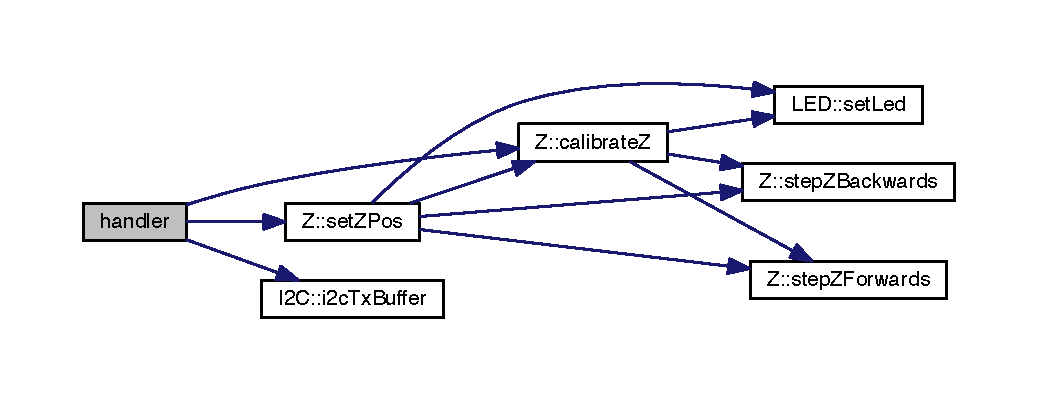
\includegraphics[width=350pt]{d2/d01/class_handler_af5be5b016b862943cd22504490acc8f4_cgraph}
\end{center}
\end{figure}




Her er kalder-\/grafen for denne funktion\+:
\nopagebreak
\begin{figure}[H]
\begin{center}
\leavevmode
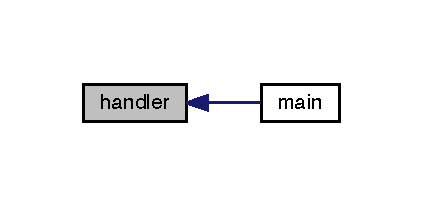
\includegraphics[width=203pt]{d2/d01/class_handler_af5be5b016b862943cd22504490acc8f4_icgraph}
\end{center}
\end{figure}




Dokumentationen for denne klasse blev genereret ud fra filerne\+:\begin{DoxyCompactItemize}
\item 
\hyperlink{handler_8h}{handler.\+h}\item 
\hyperlink{handler_8c}{handler.\+c}\end{DoxyCompactItemize}

\hypertarget{class_i2_c}{}\subsection{I2C Klasse-\/reference}
\label{class_i2_c}\index{I2C@{I2C}}


\hyperlink{class_i2_c}{I2C} class.  




{\ttfamily \#include $<$i2c.\+h$>$}



Samarbejdsdiagram for I2C\+:
\nopagebreak
\begin{figure}[H]
\begin{center}
\leavevmode
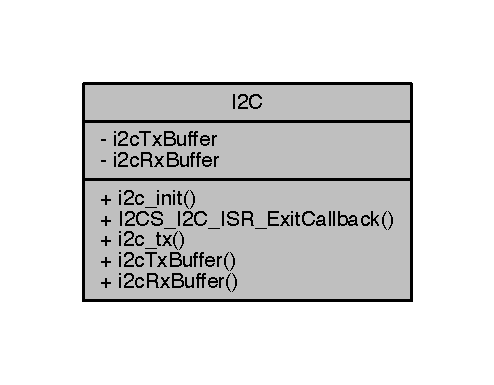
\includegraphics[width=237pt]{df/d70/class_i2_c__coll__graph}
\end{center}
\end{figure}
\subsubsection*{Offentlige metoder}
\begin{DoxyCompactItemize}
\item 
void \hyperlink{class_i2_c_a64303230bf4843297e7ac37ac236ca04}{i2c\+\_\+init} ()
\begin{DoxyCompactList}\small\item\em Initialiser \hyperlink{class_i2_c}{I2C} modulet. \end{DoxyCompactList}\item 
void \hyperlink{class_i2_c_a1b75ff104f3614357d14cee6514ad108}{I2\+C\+S\+\_\+\+I2\+C\+\_\+\+I\+S\+R\+\_\+\+Exit\+Callback} ()
\begin{DoxyCompactList}\small\item\em Motager \char`\"{}\+Exit Callback\char`\"{} fra \hyperlink{class_i2_c}{I2C}. \end{DoxyCompactList}\item 
void \hyperlink{class_i2_c_a3d3187ad377a6ca29b3fac5c809b6012}{i2c\+\_\+tx} ()
\begin{DoxyCompactList}\small\item\em Ryder om efter \hyperlink{class_i2_c}{I2C}. \end{DoxyCompactList}\item 
uint8 \hyperlink{class_i2_c_a58ba88cddd7843f12a40a87c998f00da}{i2c\+Tx\+Buffer} \mbox{[}\hyperlink{i2c_8h_a6458dbf193a0eef0470fc1b08400bfcd}{I2\+C\+\_\+\+B\+U\+F\+F\+E\+R\+\_\+\+S\+I\+ZE}\mbox{]}
\begin{DoxyCompactList}\small\item\em Buffer til afsendelse af data. \end{DoxyCompactList}\item 
uint8 \hyperlink{class_i2_c_a711782550427eea544dabe5394d79a9b}{i2c\+Rx\+Buffer} \mbox{[}\hyperlink{i2c_8h_a6458dbf193a0eef0470fc1b08400bfcd}{I2\+C\+\_\+\+B\+U\+F\+F\+E\+R\+\_\+\+S\+I\+ZE}\mbox{]}
\begin{DoxyCompactList}\small\item\em Buffer til modtagelse af data. \end{DoxyCompactList}\end{DoxyCompactItemize}
\subsubsection*{Private attributter}
\begin{DoxyCompactItemize}
\item 
uint8 \hyperlink{class_i2_c_af66ed5dc7817e74d7da731c994721217}{i2c\+Tx\+Buffer} \mbox{[}\hyperlink{i2c_8h_a6458dbf193a0eef0470fc1b08400bfcd}{I2\+C\+\_\+\+B\+U\+F\+F\+E\+R\+\_\+\+S\+I\+ZE}\mbox{]} = \{\hyperlink{i2c_8h_a52bb5b964361ed2f1b18df32c5b8f2c5}{I2\+C\+\_\+\+P\+A\+C\+K\+E\+T\+\_\+\+S\+OP}, \hyperlink{i2c_8h_aee0adbd7dcb13e95337369b7342a27e3}{I2\+C\+\_\+\+S\+T\+S\+\_\+\+C\+M\+D\+\_\+\+F\+A\+IL}, \hyperlink{i2c_8h_aee0adbd7dcb13e95337369b7342a27e3}{I2\+C\+\_\+\+S\+T\+S\+\_\+\+C\+M\+D\+\_\+\+F\+A\+IL}, \hyperlink{i2c_8h_a62b4ae6e51a3d0da47f5165165cdbc0a}{I2\+C\+\_\+\+P\+A\+C\+K\+E\+T\+\_\+\+E\+OP}\}
\begin{DoxyCompactList}\small\item\em Buffer til afsendelse af data. \end{DoxyCompactList}\item 
uint8 \hyperlink{class_i2_c_a88d6ebcf1ef5f528b63cf306ad1a5909}{i2c\+Rx\+Buffer} \mbox{[}\hyperlink{i2c_8h_a6458dbf193a0eef0470fc1b08400bfcd}{I2\+C\+\_\+\+B\+U\+F\+F\+E\+R\+\_\+\+S\+I\+ZE}\mbox{]}
\begin{DoxyCompactList}\small\item\em Buffer til modtagelse af data. \end{DoxyCompactList}\end{DoxyCompactItemize}


\subsubsection{Detaljeret beskrivelse}
\hyperlink{class_i2_c}{I2C} class. 

Håndter kommunikation via I2\+C-\/busset. \begin{DoxyAuthor}{Forfatter}
Jeppe Stærk Antonsen (\href{mailto:201271201@uni.au.dk}{\tt 201271201@uni.\+au.\+dk}) 
\end{DoxyAuthor}


\subsubsection{Dokumentation af medlemsfunktioner}
\index{I2C@{I2C}!i2c\+\_\+init@{i2c\+\_\+init}}
\index{i2c\+\_\+init@{i2c\+\_\+init}!I2C@{I2C}}
\paragraph[{\texorpdfstring{i2c\+\_\+init()}{i2c_init()}}]{\setlength{\rightskip}{0pt plus 5cm}void i2c\+\_\+init (
\begin{DoxyParamCaption}
\item[{void}]{}
\end{DoxyParamCaption}
)}\hypertarget{class_i2_c_a64303230bf4843297e7ac37ac236ca04}{}\label{class_i2_c_a64303230bf4843297e7ac37ac236ca04}


Initialiser \hyperlink{class_i2_c}{I2C} modulet. 

Initailiser \hyperlink{class_i2_c}{I2C} komponent på P\+SoC\textquotesingle{}en.

\begin{DoxyAuthor}{Forfatter}
Jeppe Stærk (\href{mailto:201271201@uni.au.dk}{\tt 201271201@uni.\+au.\+dk}) 
\end{DoxyAuthor}


Defineret på linje 49 i filen i2c.\+c.



Indeholder referencer til I2\+C\+\_\+\+B\+U\+F\+F\+E\+R\+\_\+\+S\+I\+ZE, i2c\+Rx\+Buffer() og i2c\+Tx\+Buffer().



Refereret til af main().


\begin{DoxyCode}
50 \{
51   I2CS\_I2CSlaveInitReadBuf(\hyperlink{class_i2_c_a58ba88cddd7843f12a40a87c998f00da}{i2cTxBuffer}, \hyperlink{i2c_8h_a6458dbf193a0eef0470fc1b08400bfcd}{I2C\_BUFFER\_SIZE});
52   I2CS\_I2CSlaveClearReadBuf();
53   I2CS\_I2CSlaveClearReadStatus();
54   
55   I2CS\_I2CSlaveInitWriteBuf(\hyperlink{class_i2_c_a711782550427eea544dabe5394d79a9b}{i2cRxBuffer}, \hyperlink{i2c_8h_a6458dbf193a0eef0470fc1b08400bfcd}{I2C\_BUFFER\_SIZE});
56   I2CS\_I2CSlaveClearWriteBuf();
57   I2CS\_I2CSlaveClearWriteStatus();
58   
59   I2CS\_Start();
60 \}
\end{DoxyCode}


Her er kald-\/grafen for denne funktion\+:
\nopagebreak
\begin{figure}[H]
\begin{center}
\leavevmode
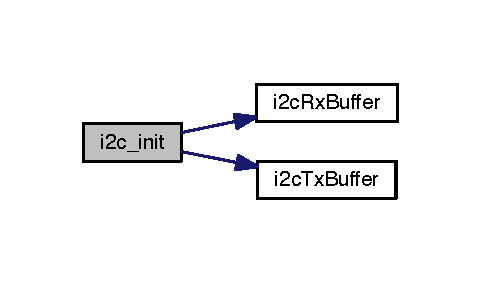
\includegraphics[width=231pt]{d4/d47/class_i2_c_a64303230bf4843297e7ac37ac236ca04_cgraph}
\end{center}
\end{figure}




Her er kalder-\/grafen for denne funktion\+:
\nopagebreak
\begin{figure}[H]
\begin{center}
\leavevmode
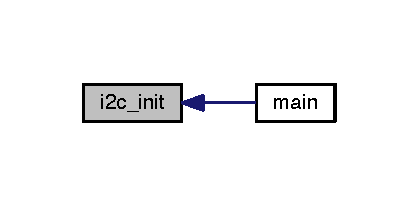
\includegraphics[width=201pt]{d4/d47/class_i2_c_a64303230bf4843297e7ac37ac236ca04_icgraph}
\end{center}
\end{figure}


\index{I2C@{I2C}!i2c\+\_\+tx@{i2c\+\_\+tx}}
\index{i2c\+\_\+tx@{i2c\+\_\+tx}!I2C@{I2C}}
\paragraph[{\texorpdfstring{i2c\+\_\+tx()}{i2c_tx()}}]{\setlength{\rightskip}{0pt plus 5cm}void i2c\+\_\+tx (
\begin{DoxyParamCaption}
\item[{void}]{}
\end{DoxyParamCaption}
)}\hypertarget{class_i2_c_a3d3187ad377a6ca29b3fac5c809b6012}{}\label{class_i2_c_a3d3187ad377a6ca29b3fac5c809b6012}


Ryder om efter \hyperlink{class_i2_c}{I2C}. 

Efter fuldført afsendelse af pakke til I2\+C-\/master, bliver status nulstillet.

\begin{DoxyAuthor}{Forfatter}
Jeppe Stærk (\href{mailto:201271201@uni.au.dk}{\tt 201271201@uni.\+au.\+dk}) 
\end{DoxyAuthor}


Defineret på linje 115 i filen i2c.\+c.



Refereret til af main().


\begin{DoxyCode}
116 \{
117   \textcolor{keywordflow}{if}(0u != (I2CS\_I2CSlaveStatus() & I2CS\_I2C\_SSTAT\_RD\_CMPLT))
118   \{
119     I2CS\_I2CSlaveClearReadBuf();
120     (void) I2CS\_I2CSlaveClearReadStatus();
121   \}
122 \}
\end{DoxyCode}


Her er kalder-\/grafen for denne funktion\+:
\nopagebreak
\begin{figure}[H]
\begin{center}
\leavevmode
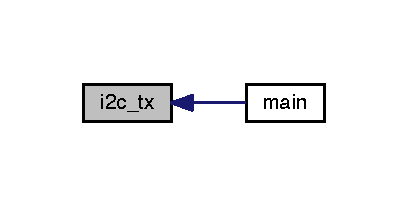
\includegraphics[width=196pt]{d4/d47/class_i2_c_a3d3187ad377a6ca29b3fac5c809b6012_icgraph}
\end{center}
\end{figure}


\index{I2C@{I2C}!i2c\+Rx\+Buffer@{i2c\+Rx\+Buffer}}
\index{i2c\+Rx\+Buffer@{i2c\+Rx\+Buffer}!I2C@{I2C}}
\paragraph[{\texorpdfstring{i2c\+Rx\+Buffer[I2\+C\+\_\+\+B\+U\+F\+F\+E\+R\+\_\+\+S\+I\+ZE]}{i2cRxBuffer[I2C_BUFFER_SIZE]}}]{\setlength{\rightskip}{0pt plus 5cm}uint8 i2c\+Rx\+Buffer (
\begin{DoxyParamCaption}
{}
\end{DoxyParamCaption}
)}\hypertarget{class_i2_c_a711782550427eea544dabe5394d79a9b}{}\label{class_i2_c_a711782550427eea544dabe5394d79a9b}


Buffer til modtagelse af data. 

En buffer der indeholder de data pakker der skal modtagelse over I2\+C-\/busset.

\begin{DoxyAuthor}{Forfatter}
Jeppe Stærk (\href{mailto:201271201@uni.au.dk}{\tt 201271201@uni.\+au.\+dk}) 
\end{DoxyAuthor}


Defineret på linje 76 i filen i2c.\+h.



Refereret til af i2c\+\_\+init() og I2\+C\+S\+\_\+\+I2\+C\+\_\+\+I\+S\+R\+\_\+\+Exit\+Callback().



Her er kalder-\/grafen for denne funktion\+:
\nopagebreak
\begin{figure}[H]
\begin{center}
\leavevmode
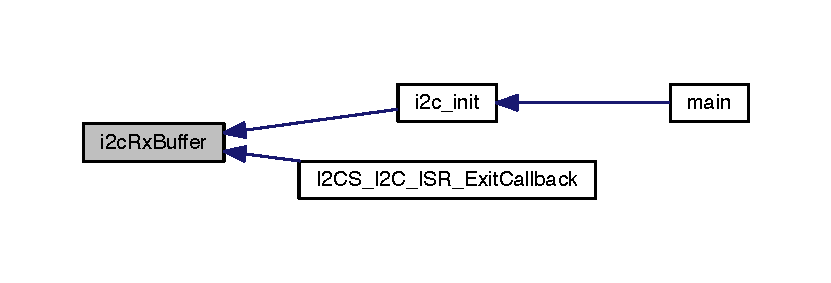
\includegraphics[width=350pt]{d4/d47/class_i2_c_a711782550427eea544dabe5394d79a9b_icgraph}
\end{center}
\end{figure}


\index{I2C@{I2C}!I2\+C\+S\+\_\+\+I2\+C\+\_\+\+I\+S\+R\+\_\+\+Exit\+Callback@{I2\+C\+S\+\_\+\+I2\+C\+\_\+\+I\+S\+R\+\_\+\+Exit\+Callback}}
\index{I2\+C\+S\+\_\+\+I2\+C\+\_\+\+I\+S\+R\+\_\+\+Exit\+Callback@{I2\+C\+S\+\_\+\+I2\+C\+\_\+\+I\+S\+R\+\_\+\+Exit\+Callback}!I2C@{I2C}}
\paragraph[{\texorpdfstring{I2\+C\+S\+\_\+\+I2\+C\+\_\+\+I\+S\+R\+\_\+\+Exit\+Callback()}{I2CS_I2C_ISR_ExitCallback()}}]{\setlength{\rightskip}{0pt plus 5cm}void I2\+C\+S\+\_\+\+I2\+C\+\_\+\+I\+S\+R\+\_\+\+Exit\+Callback (
\begin{DoxyParamCaption}
\item[{void}]{}
\end{DoxyParamCaption}
)}\hypertarget{class_i2_c_a1b75ff104f3614357d14cee6514ad108}{}\label{class_i2_c_a1b75ff104f3614357d14cee6514ad108}


Motager \char`\"{}\+Exit Callback\char`\"{} fra \hyperlink{class_i2_c}{I2C}. 

En \char`\"{}\+Interrupt Service Routine(\+I\+S\+R)\char`\"{} der aktiveres ved færdig modtagelse af kald via I2\+C-\/busset, det modtaget data behandles og håndteres.

\begin{DoxyAuthor}{Forfatter}
Jeppe Stærk (\href{mailto:201271201@uni.au.dk}{\tt 201271201@uni.\+au.\+dk}) 
\end{DoxyAuthor}


Defineret på linje 69 i filen i2c.\+c.



Indeholder referencer til Action\+::cmd, C\+M\+D\+\_\+\+S\+E\+T\+\_\+\+Z\+\_\+\+P\+OS, dataZ, I2\+C\+\_\+\+B\+U\+F\+F\+E\+R\+\_\+\+S\+I\+ZE, I2\+C\+\_\+\+P\+A\+C\+K\+E\+T\+\_\+\+C\+M\+D\+\_\+\+P\+OS, I2\+C\+\_\+\+P\+A\+C\+K\+E\+T\+\_\+\+V\+A\+L\+\_\+\+P\+OS, i2c\+Rx\+Buffer(), Data\+Z\+::isr\+StopZ, Queue\+::push\+Queue() og Action\+::val.


\begin{DoxyCode}
70 \{
71   \textcolor{keywordflow}{if}(I2CS\_I2CSlaveGetWriteBufSize() == \hyperlink{i2c_8h_a6458dbf193a0eef0470fc1b08400bfcd}{I2C\_BUFFER\_SIZE})
72   \{
73     DEBUG\_PutCRLF();
74     DEBUG\_PutString(\textcolor{stringliteral}{"** isr exit callback **"});
75     DEBUG\_PutCRLF();
76     DEBUG\_PutString(\textcolor{stringliteral}{"I> i2cRxBuffer[0]: "});
77     DEBUG\_PutHexByte(\hyperlink{class_i2_c_a711782550427eea544dabe5394d79a9b}{i2cRxBuffer}[0]);
78     DEBUG\_PutString(\textcolor{stringliteral}{" [1]: "});
79     DEBUG\_PutHexByte(\hyperlink{class_i2_c_a711782550427eea544dabe5394d79a9b}{i2cRxBuffer}[1]);
80     DEBUG\_PutString(\textcolor{stringliteral}{" [2]: "});
81     DEBUG\_PutHexByte(\hyperlink{class_i2_c_a711782550427eea544dabe5394d79a9b}{i2cRxBuffer}[2]);
82     DEBUG\_PutString(\textcolor{stringliteral}{" [3]: "});
83     DEBUG\_PutHexByte(\hyperlink{class_i2_c_a711782550427eea544dabe5394d79a9b}{i2cRxBuffer}[3]);
84     DEBUG\_PutString(\textcolor{stringliteral}{" buffer size: "});
85     DEBUG\_PutHexByte(I2CS\_I2CSlaveGetWriteBufSize());
86     DEBUG\_PutCRLF();
87     
88     \textcolor{keyword}{struct }\hyperlink{queue_8h_df/d8c/struct_action}{Action} action;
89     action.\hyperlink{queue_8h_a85092d82ab6ea85dad51ba78cbda36a0}{cmd} = \hyperlink{class_i2_c_a711782550427eea544dabe5394d79a9b}{i2cRxBuffer}[\hyperlink{i2c_8h_ac13fcfeded7dc2d82fa4734456f3761f}{I2C\_PACKET\_CMD\_POS}];
90     action.val = \hyperlink{class_i2_c_a711782550427eea544dabe5394d79a9b}{i2cRxBuffer}[\hyperlink{i2c_8h_a68506c3651f015716bb2c135e8e7b972}{I2C\_PACKET\_VAL\_POS}];
91     
92     \textcolor{keywordflow}{switch}(\hyperlink{class_i2_c_a711782550427eea544dabe5394d79a9b}{i2cRxBuffer}[\hyperlink{i2c_8h_ac13fcfeded7dc2d82fa4734456f3761f}{I2C\_PACKET\_CMD\_POS}]) \{
93       \textcolor{keywordflow}{case} \hyperlink{handler_8h_a6e695093ea021ccac7cc5d2d788095c9}{CMD\_SET\_Z\_POS} :
94         \hyperlink{data_8h_ace1aa5b973b9358f7236c0c9deca9370}{dataZ}.\hyperlink{data_8h_ae55ff8378d0a07b118000a98b273141f}{isrStopZ} = 1;
95         DEBUG\_PutString(\textcolor{stringliteral}{") isrStopZ = 1"});
96         DEBUG\_PutCRLF();
97         \hyperlink{queue_8h_a0012fa831aa1529e5ed3a6610b733423}{pushQueue}(action);
98         \textcolor{keywordflow}{break};
99       \textcolor{keywordflow}{default} :
100         \hyperlink{queue_8h_a0012fa831aa1529e5ed3a6610b733423}{pushQueue}(action);
101         \textcolor{keywordflow}{break};
102     \}
103     I2CS\_I2CSlaveClearWriteBuf();
104     (void) I2CS\_I2CSlaveClearWriteStatus();
105   \}
106 \}
\end{DoxyCode}


Her er kald-\/grafen for denne funktion\+:
\nopagebreak
\begin{figure}[H]
\begin{center}
\leavevmode
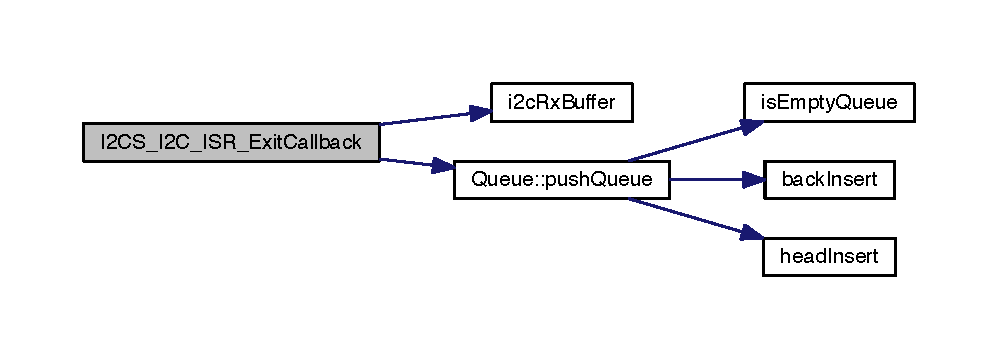
\includegraphics[width=350pt]{d4/d47/class_i2_c_a1b75ff104f3614357d14cee6514ad108_cgraph}
\end{center}
\end{figure}


\index{I2C@{I2C}!i2c\+Tx\+Buffer@{i2c\+Tx\+Buffer}}
\index{i2c\+Tx\+Buffer@{i2c\+Tx\+Buffer}!I2C@{I2C}}
\paragraph[{\texorpdfstring{i2c\+Tx\+Buffer[I2\+C\+\_\+\+B\+U\+F\+F\+E\+R\+\_\+\+S\+I\+ZE]}{i2cTxBuffer[I2C_BUFFER_SIZE]}}]{\setlength{\rightskip}{0pt plus 5cm}uint8 i2c\+Tx\+Buffer (
\begin{DoxyParamCaption}
{}
\end{DoxyParamCaption}
)}\hypertarget{class_i2_c_a58ba88cddd7843f12a40a87c998f00da}{}\label{class_i2_c_a58ba88cddd7843f12a40a87c998f00da}


Buffer til afsendelse af data. 

En buffer der indeholder de data pakker der skal sende over I2\+C-\/busset.

\begin{DoxyAuthor}{Forfatter}
Jeppe Stærk (\href{mailto:201271201@uni.au.dk}{\tt 201271201@uni.\+au.\+dk}) 
\end{DoxyAuthor}


Defineret på linje 67 i filen i2c.\+h.



Refereret til af Handler\+::handler() og i2c\+\_\+init().



Her er kalder-\/grafen for denne funktion\+:
\nopagebreak
\begin{figure}[H]
\begin{center}
\leavevmode
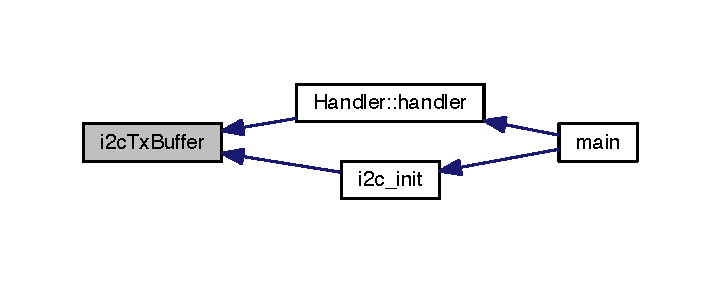
\includegraphics[width=346pt]{d4/d47/class_i2_c_a58ba88cddd7843f12a40a87c998f00da_icgraph}
\end{center}
\end{figure}




\subsubsection{Felt-\/dokumentation}
\index{I2C@{I2C}!i2c\+Rx\+Buffer@{i2c\+Rx\+Buffer}}
\index{i2c\+Rx\+Buffer@{i2c\+Rx\+Buffer}!I2C@{I2C}}
\paragraph[{\texorpdfstring{i2c\+Rx\+Buffer}{i2cRxBuffer}}]{\setlength{\rightskip}{0pt plus 5cm}uint8 i2c\+Rx\+Buffer\mbox{[}{\bf I2\+C\+\_\+\+B\+U\+F\+F\+E\+R\+\_\+\+S\+I\+ZE}\mbox{]}\hspace{0.3cm}{\ttfamily [private]}}\hypertarget{class_i2_c_a88d6ebcf1ef5f528b63cf306ad1a5909}{}\label{class_i2_c_a88d6ebcf1ef5f528b63cf306ad1a5909}


Buffer til modtagelse af data. 

En buffer der indeholder de data pakker der skal modtagelse over I2\+C-\/busset.

\begin{DoxyAuthor}{Forfatter}
Jeppe Stærk (\href{mailto:201271201@uni.au.dk}{\tt 201271201@uni.\+au.\+dk}) 
\end{DoxyAuthor}


Defineret på linje 35 i filen i2c.\+c.

\index{I2C@{I2C}!i2c\+Tx\+Buffer@{i2c\+Tx\+Buffer}}
\index{i2c\+Tx\+Buffer@{i2c\+Tx\+Buffer}!I2C@{I2C}}
\paragraph[{\texorpdfstring{i2c\+Tx\+Buffer}{i2cTxBuffer}}]{\setlength{\rightskip}{0pt plus 5cm}uint8 i2c\+Tx\+Buffer\mbox{[}{\bf I2\+C\+\_\+\+B\+U\+F\+F\+E\+R\+\_\+\+S\+I\+ZE}\mbox{]} = \{{\bf I2\+C\+\_\+\+P\+A\+C\+K\+E\+T\+\_\+\+S\+OP}, {\bf I2\+C\+\_\+\+S\+T\+S\+\_\+\+C\+M\+D\+\_\+\+F\+A\+IL}, {\bf I2\+C\+\_\+\+S\+T\+S\+\_\+\+C\+M\+D\+\_\+\+F\+A\+IL}, {\bf I2\+C\+\_\+\+P\+A\+C\+K\+E\+T\+\_\+\+E\+OP}\}\hspace{0.3cm}{\ttfamily [private]}}\hypertarget{class_i2_c_af66ed5dc7817e74d7da731c994721217}{}\label{class_i2_c_af66ed5dc7817e74d7da731c994721217}


Buffer til afsendelse af data. 

En buffer der indeholder de data pakker der skal sende over I2\+C-\/busset.

\begin{DoxyAuthor}{Forfatter}
Jeppe Stærk (\href{mailto:201271201@uni.au.dk}{\tt 201271201@uni.\+au.\+dk}) 
\end{DoxyAuthor}


Defineret på linje 26 i filen i2c.\+c.



Dokumentationen for denne klasse blev genereret ud fra filerne\+:\begin{DoxyCompactItemize}
\item 
\hyperlink{i2c_8h}{i2c.\+h}\item 
\hyperlink{i2c_8c}{i2c.\+c}\end{DoxyCompactItemize}

\hypertarget{class_l_e_d}{}\subsection{L\+ED Klasse-\/reference}
\label{class_l_e_d}\index{L\+ED@{L\+ED}}


\hyperlink{class_l_e_d}{L\+ED} class.  




{\ttfamily \#include $<$led.\+h$>$}



Samarbejdsdiagram for L\+ED\+:\nopagebreak
\begin{figure}[H]
\begin{center}
\leavevmode
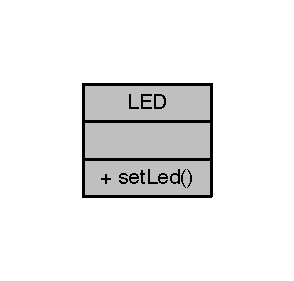
\includegraphics[width=141pt]{d3/df9/class_l_e_d__coll__graph}
\end{center}
\end{figure}
\subsubsection*{Offentlige metoder}
\begin{DoxyCompactItemize}
\item 
void \hyperlink{class_l_e_d_a1d8e725e3829da99c1d027ba0a2ce57a}{set\+Led} (uint8 red, uint8 green, uint8 blue, uint8 delay)
\begin{DoxyCompactList}\small\item\em Sætter den defineret farve og angivet delay. \end{DoxyCompactList}\end{DoxyCompactItemize}


\subsubsection{Detaljeret beskrivelse}
\hyperlink{class_l_e_d}{L\+ED} class. 

Håndtere P\+SoC\textquotesingle{}ens røde, grønne og blå led \begin{DoxyAuthor}{Forfatter}
Casper Dieu Le (\href{mailto:201370338@uni.au.dk}{\tt 201370338@uni.\+au.\+dk}) 

Kasper Hinkler Uldbjerg (\href{mailto:201370281@uni.au.dk}{\tt 201370281@uni.\+au.\+dk}) 

Jeppe Stærk Antonsen (\href{mailto:201271201@uni.au.dk}{\tt 201271201@uni.\+au.\+dk}) 
\end{DoxyAuthor}


\subsubsection{Dokumentation af medlemsfunktioner}
\index{L\+ED@{L\+ED}!set\+Led@{set\+Led}}
\index{set\+Led@{set\+Led}!L\+ED@{L\+ED}}
\paragraph[{\texorpdfstring{set\+Led(uint8 red, uint8 green, uint8 blue, uint8 delay)}{setLed(uint8 red, uint8 green, uint8 blue, uint8 delay)}}]{\setlength{\rightskip}{0pt plus 5cm}void set\+Led (
\begin{DoxyParamCaption}
\item[{uint8}]{red, }
\item[{uint8}]{green, }
\item[{uint8}]{blue, }
\item[{uint8}]{delay}
\end{DoxyParamCaption}
)}\hypertarget{class_l_e_d_a1d8e725e3829da99c1d027ba0a2ce57a}{}\label{class_l_e_d_a1d8e725e3829da99c1d027ba0a2ce57a}


Sætter den defineret farve og angivet delay. 

Metoden sætter den/de valgte farver og venter i det angivet delay. 
\begin{DoxyParams}[1]{Parametre}
\mbox{\tt in}  & {\em red} & Tænder/slukker den røde led. \\
\hline
\mbox{\tt in}  & {\em green} & Tænder/slukker den grønne led. \\
\hline
\mbox{\tt in}  & {\em blue} & Tænder/slukker den blå led. \\
\hline
\mbox{\tt in}  & {\em delay} & Tid i microsekunder til delay.\\
\hline
\end{DoxyParams}
\begin{DoxyAuthor}{Forfatter}
Casper Dieu Le (\href{mailto:201370338@uni.au.dk}{\tt 201370338@uni.\+au.\+dk}) 

Kasper Hinkler Uldbjerg (\href{mailto:201370281@uni.au.dk}{\tt 201370281@uni.\+au.\+dk}) 

Jeppe Stærk (\href{mailto:201271201@uni.au.dk}{\tt 201271201@uni.\+au.\+dk}) 
\end{DoxyAuthor}


Defineret på linje 28 i filen led.\+c.



Indeholder referencer til L\+E\+D\+\_\+\+O\+FF og L\+E\+D\+\_\+\+ON.



Refereret til af X\+Y\+::calibrate\+X(), X\+Y\+::calibrate\+Y(), X\+Y\+::\+C\+Y\+\_\+\+I\+S\+R(), main(), X\+Y\+::set\+X\+Pos() og X\+Y\+::set\+Y\+Pos().


\begin{DoxyCode}
29 \{
30   red ? LED\_RED\_Write(\hyperlink{led_8h_af2e697ac60e05813d45ea2c9c9e79c25}{LED\_ON}) : LED\_RED\_Write(\hyperlink{led_8h_a80700bb63bd56ebabbb4728aa433fd29}{LED\_OFF});
31   green ? LED\_GREEN\_Write(\hyperlink{led_8h_af2e697ac60e05813d45ea2c9c9e79c25}{LED\_ON}) : LED\_GREEN\_Write(\hyperlink{led_8h_a80700bb63bd56ebabbb4728aa433fd29}{LED\_OFF});
32   blue ? LED\_BLUE\_Write(\hyperlink{led_8h_af2e697ac60e05813d45ea2c9c9e79c25}{LED\_ON}) : LED\_BLUE\_Write(\hyperlink{led_8h_a80700bb63bd56ebabbb4728aa433fd29}{LED\_OFF});
33   
34   CyDelay(delay);
35 \}
\end{DoxyCode}


Her er kalder-\/grafen for denne funktion\+:\nopagebreak
\begin{figure}[H]
\begin{center}
\leavevmode
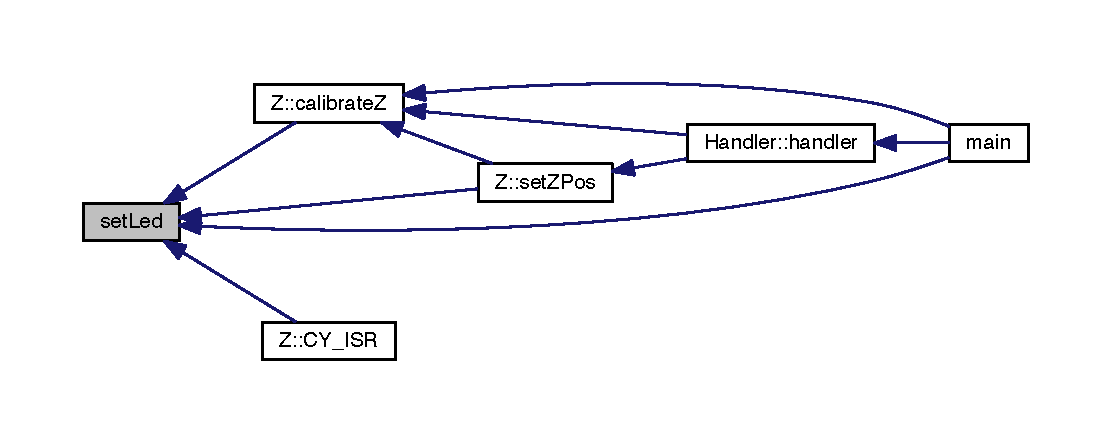
\includegraphics[width=350pt]{d3/dbe/class_l_e_d_a1d8e725e3829da99c1d027ba0a2ce57a_icgraph}
\end{center}
\end{figure}




Dokumentationen for denne klasse blev genereret ud fra filerne\+:\begin{DoxyCompactItemize}
\item 
\hyperlink{led_8h}{led.\+h}\item 
\hyperlink{led_8c}{led.\+c}\end{DoxyCompactItemize}

\hypertarget{class_queue}{}\subsection{Queue Klasse-\/reference}
\label{class_queue}\index{Queue@{Queue}}


\hyperlink{class_queue}{Queue} class.  




{\ttfamily \#include $<$queue.\+h$>$}



Samarbejdsdiagram for Queue\+:
\nopagebreak
\begin{figure}[H]
\begin{center}
\leavevmode
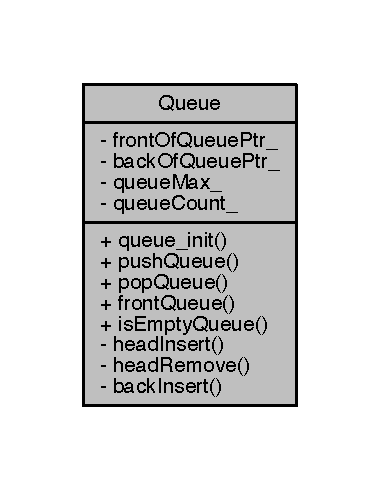
\includegraphics[width=182pt]{d9/d28/class_queue__coll__graph}
\end{center}
\end{figure}
\subsubsection*{Offentlige metoder}
\begin{DoxyCompactItemize}
\item 
void \hyperlink{class_queue_a4e0a3758d721506e7729f4d074a280ff}{queue\+\_\+init} (uint8 queue\+Max\+Size)
\begin{DoxyCompactList}\small\item\em Initialiser \hyperlink{class_queue}{Queue} modulet. \end{DoxyCompactList}\item 
void \hyperlink{class_queue_a0012fa831aa1529e5ed3a6610b733423}{push\+Queue} (const struct \hyperlink{queue_8h_df/d8c/struct_action}{Action} data)
\begin{DoxyCompactList}\small\item\em Indsætter et element i køen. \end{DoxyCompactList}\item 
void \hyperlink{class_queue_a9ecab9ecdedfc331aed9a0ae63ce193b}{pop\+Queue} ()
\begin{DoxyCompactList}\small\item\em Fjerner et element i køen. \end{DoxyCompactList}\item 
struct \hyperlink{queue_8h_df/d8c/struct_action}{Action} \hyperlink{class_queue_a49c50ba30a42033068d8d8e6a23c6ca1}{front\+Queue} ()
\begin{DoxyCompactList}\small\item\em Viser et element fra køen. \end{DoxyCompactList}\item 
uint8 \hyperlink{class_queue_aafb324c79731abdc228dbf94d86722a3}{is\+Empty\+Queue} ()
\begin{DoxyCompactList}\small\item\em Retuner status af køen. \end{DoxyCompactList}\end{DoxyCompactItemize}
\subsubsection*{Private metoder}
\begin{DoxyCompactItemize}
\item 
void \hyperlink{class_queue_a1189c09234d75518492525645a05db07}{head\+Insert} (struct \hyperlink{queue_8c_db/d8b/struct_node}{Node} $\ast$$\ast$head\+Ptr, const struct \hyperlink{queue_8h_df/d8c/struct_action}{Action} data)
\begin{DoxyCompactList}\small\item\em Indsætter forreste i listen. \end{DoxyCompactList}\item 
void \hyperlink{class_queue_ae54666c891fd21d5497f48c385a00b74}{head\+Remove} (struct \hyperlink{queue_8c_db/d8b/struct_node}{Node} $\ast$$\ast$head\+Ptr)
\begin{DoxyCompactList}\small\item\em Fjerner fra listen. \end{DoxyCompactList}\item 
void \hyperlink{class_queue_a5a25a737ba7dff74923f5cb04e19164c}{back\+Insert} (struct \hyperlink{queue_8c_db/d8b/struct_node}{Node} $\ast$$\ast$back\+Ptr, const struct \hyperlink{queue_8h_df/d8c/struct_action}{Action} data)
\begin{DoxyCompactList}\small\item\em Indsætter bagerst i listen. \end{DoxyCompactList}\end{DoxyCompactItemize}
\subsubsection*{Statiske, private attributter}
\begin{DoxyCompactItemize}
\item 
static struct \hyperlink{queue_8c_db/d8b/struct_node}{Node} $\ast$ \hyperlink{class_queue_aa48f05218d0a78402821c8aa9bdad06a}{front\+Of\+Queue\+Ptr\+\_\+}
\begin{DoxyCompactList}\small\item\em Pointer til foreste element i køen. \end{DoxyCompactList}\item 
static struct \hyperlink{queue_8c_db/d8b/struct_node}{Node} $\ast$ \hyperlink{class_queue_a225d2c9ad4e83d6da443e99b8869a51c}{back\+Of\+Queue\+Ptr\+\_\+}
\begin{DoxyCompactList}\small\item\em Pointer til bagerste element i køen. \end{DoxyCompactList}\item 
static uint8 \hyperlink{class_queue_acb6b6e88c9e4d12839594b31e6ff7c5a}{queue\+Max\+\_\+}
\begin{DoxyCompactList}\small\item\em Køens max. \end{DoxyCompactList}\item 
static uint8 \hyperlink{class_queue_ad260f9ccca00e80d161bbf3e70c3ffa6}{queue\+Count\+\_\+}
\begin{DoxyCompactList}\small\item\em Kø element tæller. \end{DoxyCompactList}\end{DoxyCompactItemize}


\subsubsection{Detaljeret beskrivelse}
\hyperlink{class_queue}{Queue} class. 

En F\+I\+FO kø der er opbygget af en single linket liste. \begin{DoxyAuthor}{Forfatter}
Jeppe Stærk Antonsen (\href{mailto:201271201@uni.au.dk}{\tt 201271201@uni.\+au.\+dk}) 
\end{DoxyAuthor}


\subsubsection{Dokumentation af medlemsfunktioner}
\index{Queue@{Queue}!back\+Insert@{back\+Insert}}
\index{back\+Insert@{back\+Insert}!Queue@{Queue}}
\paragraph[{\texorpdfstring{back\+Insert(struct Node $\ast$$\ast$back\+Ptr, const struct Action data)}{backInsert(struct Node **backPtr, const struct Action data)}}]{\setlength{\rightskip}{0pt plus 5cm}void back\+Insert (
\begin{DoxyParamCaption}
\item[{struct {\bf Node} $\ast$$\ast$}]{back\+Ptr, }
\item[{const struct {\bf Action}}]{data}
\end{DoxyParamCaption}
)\hspace{0.3cm}{\ttfamily [private]}}\hypertarget{class_queue_a5a25a737ba7dff74923f5cb04e19164c}{}\label{class_queue_a5a25a737ba7dff74923f5cb04e19164c}


Indsætter bagerst i listen. 

Indsætter det angivet element bagerst i den underlægende linked liste. 
\begin{DoxyParams}[1]{Parametre}
\mbox{\tt in}  & {\em back\+Ptr} & Pointer til det bagerste element i listen. \\
\hline
\mbox{\tt in}  & {\em data} & \hyperlink{class_data}{Data} der skal indsættes i listen.\\
\hline
\end{DoxyParams}
\begin{DoxyAuthor}{Forfatter}
Jeppe Stærk Antonsen (\href{mailto:201271201@uni.au.dk}{\tt 201271201@uni.\+au.\+dk}) 
\end{DoxyAuthor}


Defineret på linje 248 i filen queue.\+c.



Indeholder referencer til Node\+::data\+\_\+ og Node\+::next\+\_\+.


\begin{DoxyCode}
249 \{
250   \textcolor{keywordflow}{if}(*backPtr == NULL)
251   \{
252     \textcolor{keywordflow}{return};
253   \}
254   
255   \textcolor{keyword}{struct }\hyperlink{queue_8c_db/d8b/struct_node}{Node}* next = (*backPtr)->\hyperlink{queue_8c_a882bca6dea645e11ca1df6bc3c30ac42}{next\_};
256   \textcolor{keyword}{struct }\hyperlink{queue_8c_db/d8b/struct_node}{Node}* temp = (\textcolor{keyword}{struct }\hyperlink{queue_8c_db/d8b/struct_node}{Node}*)malloc(\textcolor{keyword}{sizeof}(\textcolor{keyword}{struct} \hyperlink{queue_8c_db/d8b/struct_node}{Node}));
257   temp->\hyperlink{queue_8c_ab134027ce40d71eaa8746f6a8e7d4b8a}{data\_} = data;
258   temp->\hyperlink{queue_8c_a882bca6dea645e11ca1df6bc3c30ac42}{next\_} = next;
259   (*backPtr)->\hyperlink{queue_8c_a882bca6dea645e11ca1df6bc3c30ac42}{next\_} = temp;
260 \}
\end{DoxyCode}
\index{Queue@{Queue}!front\+Queue@{front\+Queue}}
\index{front\+Queue@{front\+Queue}!Queue@{Queue}}
\paragraph[{\texorpdfstring{front\+Queue()}{frontQueue()}}]{\setlength{\rightskip}{0pt plus 5cm}struct {\bf Action} front\+Queue (
\begin{DoxyParamCaption}
\item[{void}]{}
\end{DoxyParamCaption}
)}\hypertarget{class_queue_a49c50ba30a42033068d8d8e6a23c6ca1}{}\label{class_queue_a49c50ba30a42033068d8d8e6a23c6ca1}


Viser et element fra køen. 

Viser det foreste element i F\+I\+FO køen.

\begin{DoxyAuthor}{Forfatter}
Jeppe Stærk Antonsen (\href{mailto:201271201@uni.au.dk}{\tt 201271201@uni.\+au.\+dk}) 
\end{DoxyAuthor}


Defineret på linje 170 i filen queue.\+c.



Indeholder referencer til Node\+::data\+\_\+.



Refereret til af main().


\begin{DoxyCode}
171 \{
172   DEBUG\_PutString(\textcolor{stringliteral}{"Q=: count: "});
173   DEBUG\_PutHexByte(\hyperlink{class_queue_ad260f9ccca00e80d161bbf3e70c3ffa6}{queueCount\_});
174   DEBUG\_PutCRLF();
175   \textcolor{keywordflow}{return} \hyperlink{class_queue_aa48f05218d0a78402821c8aa9bdad06a}{frontOfQueuePtr\_}->\hyperlink{queue_8c_ab134027ce40d71eaa8746f6a8e7d4b8a}{data\_};
176 \}
\end{DoxyCode}


Her er kalder-\/grafen for denne funktion\+:
\nopagebreak
\begin{figure}[H]
\begin{center}
\leavevmode
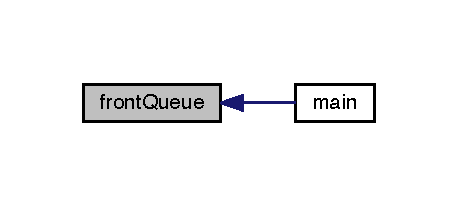
\includegraphics[width=220pt]{d4/da4/class_queue_a49c50ba30a42033068d8d8e6a23c6ca1_icgraph}
\end{center}
\end{figure}


\index{Queue@{Queue}!head\+Insert@{head\+Insert}}
\index{head\+Insert@{head\+Insert}!Queue@{Queue}}
\paragraph[{\texorpdfstring{head\+Insert(struct Node $\ast$$\ast$head\+Ptr, const struct Action data)}{headInsert(struct Node **headPtr, const struct Action data)}}]{\setlength{\rightskip}{0pt plus 5cm}void head\+Insert (
\begin{DoxyParamCaption}
\item[{struct {\bf Node} $\ast$$\ast$}]{head\+Ptr, }
\item[{const struct {\bf Action}}]{data}
\end{DoxyParamCaption}
)\hspace{0.3cm}{\ttfamily [private]}}\hypertarget{class_queue_a1189c09234d75518492525645a05db07}{}\label{class_queue_a1189c09234d75518492525645a05db07}


Indsætter forreste i listen. 

Indsætter det angivet element forreste i den underlægende linked liste. 
\begin{DoxyParams}[1]{Parametre}
\mbox{\tt in}  & {\em head\+Ptr} & Pointer til det foreste element i listen. \\
\hline
\mbox{\tt in}  & {\em data} & \hyperlink{class_data}{Data} der skal indsættes i listen.\\
\hline
\end{DoxyParams}
\begin{DoxyAuthor}{Forfatter}
Jeppe Stærk Antonsen (\href{mailto:201271201@uni.au.dk}{\tt 201271201@uni.\+au.\+dk}) 
\end{DoxyAuthor}


Defineret på linje 206 i filen queue.\+c.



Indeholder referencer til Node\+::data\+\_\+ og Node\+::next\+\_\+.


\begin{DoxyCode}
207 \{
208   \textcolor{keyword}{struct }\hyperlink{queue_8c_db/d8b/struct_node}{Node}* temp = (\textcolor{keyword}{struct }\hyperlink{queue_8c_db/d8b/struct_node}{Node}*)malloc(\textcolor{keyword}{sizeof}(\textcolor{keyword}{struct} \hyperlink{queue_8c_db/d8b/struct_node}{Node}));
209   \textcolor{keywordflow}{if}(temp == NULL)
210   \{
211     \textcolor{keywordflow}{return};
212   \}
213   
214   temp->\hyperlink{queue_8c_ab134027ce40d71eaa8746f6a8e7d4b8a}{data\_} = data;
215   temp->\hyperlink{queue_8c_a882bca6dea645e11ca1df6bc3c30ac42}{next\_} = NULL;
216   
217   *headPtr = temp;
218 \}
\end{DoxyCode}
\index{Queue@{Queue}!head\+Remove@{head\+Remove}}
\index{head\+Remove@{head\+Remove}!Queue@{Queue}}
\paragraph[{\texorpdfstring{head\+Remove(struct Node $\ast$$\ast$head\+Ptr)}{headRemove(struct Node **headPtr)}}]{\setlength{\rightskip}{0pt plus 5cm}void head\+Remove (
\begin{DoxyParamCaption}
\item[{struct {\bf Node} $\ast$$\ast$}]{head\+Ptr}
\end{DoxyParamCaption}
)\hspace{0.3cm}{\ttfamily [private]}}\hypertarget{class_queue_ae54666c891fd21d5497f48c385a00b74}{}\label{class_queue_ae54666c891fd21d5497f48c385a00b74}


Fjerner fra listen. 

Fjerner det forreste element i den underlæggende linked liste 
\begin{DoxyParams}[1]{Parametre}
\mbox{\tt in}  & {\em head\+Ptr} & Pointer til det forreste element i listen.\\
\hline
\end{DoxyParams}
\begin{DoxyAuthor}{Forfatter}
Jeppe Stærk Antonsen (\href{mailto:201271201@uni.au.dk}{\tt 201271201@uni.\+au.\+dk}) 
\end{DoxyAuthor}


Defineret på linje 228 i filen queue.\+c.



Indeholder referencer til Node\+::next\+\_\+.


\begin{DoxyCode}
229 \{
230   \textcolor{keywordflow}{if}(headPtr != NULL)
231   \{
232     \textcolor{keyword}{struct }\hyperlink{queue_8c_db/d8b/struct_node}{Node}* condemned;
233     condemned = *headPtr;
234     *headPtr = (*headPtr)->\hyperlink{queue_8c_a882bca6dea645e11ca1df6bc3c30ac42}{next\_};
235     free(condemned);
236   \}
237 \}
\end{DoxyCode}
\index{Queue@{Queue}!is\+Empty\+Queue@{is\+Empty\+Queue}}
\index{is\+Empty\+Queue@{is\+Empty\+Queue}!Queue@{Queue}}
\paragraph[{\texorpdfstring{is\+Empty\+Queue()}{isEmptyQueue()}}]{\setlength{\rightskip}{0pt plus 5cm}uint8 is\+Empty\+Queue (
\begin{DoxyParamCaption}
\item[{void}]{}
\end{DoxyParamCaption}
)}\hypertarget{class_queue_aafb324c79731abdc228dbf94d86722a3}{}\label{class_queue_aafb324c79731abdc228dbf94d86722a3}


Retuner status af køen. 

Kontrollere om køen er tom.

\begin{DoxyAuthor}{Forfatter}
Jeppe Stærk Antonsen (\href{mailto:201271201@uni.au.dk}{\tt 201271201@uni.\+au.\+dk}) 
\end{DoxyAuthor}


Defineret på linje 185 i filen queue.\+c.



Refereret til af main().


\begin{DoxyCode}
186 \{
187   \textcolor{keywordflow}{if}(\hyperlink{class_queue_aa48f05218d0a78402821c8aa9bdad06a}{frontOfQueuePtr\_} == NULL)
188   \{
189     \textcolor{keywordflow}{return} 1;
190   \}
191   \textcolor{keywordflow}{else}
192   \{
193     \textcolor{keywordflow}{return} 0;
194   \}
195 \}
\end{DoxyCode}


Her er kalder-\/grafen for denne funktion\+:
\nopagebreak
\begin{figure}[H]
\begin{center}
\leavevmode
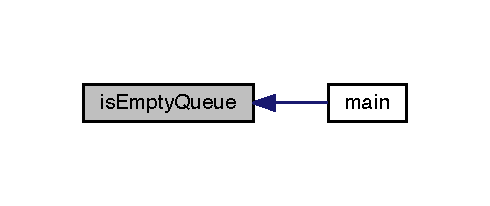
\includegraphics[width=235pt]{d4/da4/class_queue_aafb324c79731abdc228dbf94d86722a3_icgraph}
\end{center}
\end{figure}


\index{Queue@{Queue}!pop\+Queue@{pop\+Queue}}
\index{pop\+Queue@{pop\+Queue}!Queue@{Queue}}
\paragraph[{\texorpdfstring{pop\+Queue()}{popQueue()}}]{\setlength{\rightskip}{0pt plus 5cm}void pop\+Queue (
\begin{DoxyParamCaption}
\item[{void}]{}
\end{DoxyParamCaption}
)}\hypertarget{class_queue_a9ecab9ecdedfc331aed9a0ae63ce193b}{}\label{class_queue_a9ecab9ecdedfc331aed9a0ae63ce193b}


Fjerner et element i køen. 

Fjerner det foreste element i F\+I\+FO køen.

\begin{DoxyAuthor}{Forfatter}
Jeppe Stærk Antonsen (\href{mailto:201271201@uni.au.dk}{\tt 201271201@uni.\+au.\+dk}) 
\end{DoxyAuthor}


Defineret på linje 149 i filen queue.\+c.



Indeholder referencer til head\+Remove() og is\+Empty\+Queue().



Refereret til af main().


\begin{DoxyCode}
150 \{
151   \hyperlink{class_queue_ae54666c891fd21d5497f48c385a00b74}{headRemove}(&\hyperlink{class_queue_aa48f05218d0a78402821c8aa9bdad06a}{frontOfQueuePtr\_});
152   \hyperlink{class_queue_ad260f9ccca00e80d161bbf3e70c3ffa6}{queueCount\_}--;
153   \textcolor{keywordflow}{if}(\hyperlink{class_queue_aafb324c79731abdc228dbf94d86722a3}{isEmptyQueue}() == 1)
154   \{
155     \hyperlink{class_queue_a225d2c9ad4e83d6da443e99b8869a51c}{backOfQueuePtr\_} = NULL;
156   \}
157   DEBUG\_PutString(\textcolor{stringliteral}{"-Q: count: "});
158   DEBUG\_PutHexByte(\hyperlink{class_queue_ad260f9ccca00e80d161bbf3e70c3ffa6}{queueCount\_});
159   DEBUG\_PutCRLF();
160   DEBUG\_PutCRLF();
161 \}
\end{DoxyCode}


Her er kald-\/grafen for denne funktion\+:
\nopagebreak
\begin{figure}[H]
\begin{center}
\leavevmode
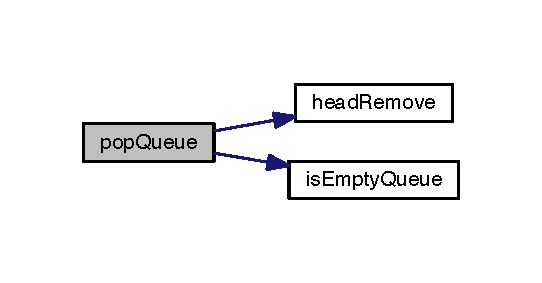
\includegraphics[width=260pt]{d4/da4/class_queue_a9ecab9ecdedfc331aed9a0ae63ce193b_cgraph}
\end{center}
\end{figure}




Her er kalder-\/grafen for denne funktion\+:
\nopagebreak
\begin{figure}[H]
\begin{center}
\leavevmode
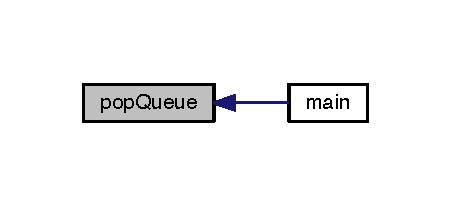
\includegraphics[width=216pt]{d4/da4/class_queue_a9ecab9ecdedfc331aed9a0ae63ce193b_icgraph}
\end{center}
\end{figure}


\index{Queue@{Queue}!push\+Queue@{push\+Queue}}
\index{push\+Queue@{push\+Queue}!Queue@{Queue}}
\paragraph[{\texorpdfstring{push\+Queue(const struct Action data)}{pushQueue(const struct Action data)}}]{\setlength{\rightskip}{0pt plus 5cm}void push\+Queue (
\begin{DoxyParamCaption}
\item[{const struct {\bf Action}}]{data}
\end{DoxyParamCaption}
)}\hypertarget{class_queue_a0012fa831aa1529e5ed3a6610b733423}{}\label{class_queue_a0012fa831aa1529e5ed3a6610b733423}


Indsætter et element i køen. 

Indsætter det angivet element bagerst i F\+I\+FO køen. 
\begin{DoxyParams}[1]{Parametre}
\mbox{\tt in}  & {\em data} & \hyperlink{class_data}{Data} der skal indsættes i køen.\\
\hline
\end{DoxyParams}
\begin{DoxyAuthor}{Forfatter}
Jeppe Stærk Antonsen (\href{mailto:201271201@uni.au.dk}{\tt 201271201@uni.\+au.\+dk}) 
\end{DoxyAuthor}


Defineret på linje 107 i filen queue.\+c.



Indeholder referencer til back\+Insert(), Action\+::cmd, head\+Insert(), is\+Empty\+Queue(), Node\+::next\+\_\+ og Action\+::val.



Refereret til af I2\+C\+::\+I2\+C\+S\+\_\+\+I2\+C\+\_\+\+I\+S\+R\+\_\+\+Exit\+Callback().


\begin{DoxyCode}
108 \{
109   \textcolor{keywordflow}{if}(\hyperlink{class_queue_ad260f9ccca00e80d161bbf3e70c3ffa6}{queueCount\_}<\hyperlink{class_queue_acb6b6e88c9e4d12839594b31e6ff7c5a}{queueMax\_})
110   \{
111     \textcolor{keywordflow}{if}(\hyperlink{class_queue_aafb324c79731abdc228dbf94d86722a3}{isEmptyQueue}() != 1)
112     \{
113       \hyperlink{class_queue_a5a25a737ba7dff74923f5cb04e19164c}{backInsert}(&\hyperlink{class_queue_a225d2c9ad4e83d6da443e99b8869a51c}{backOfQueuePtr\_}, data);
114       \hyperlink{class_queue_a225d2c9ad4e83d6da443e99b8869a51c}{backOfQueuePtr\_} = \hyperlink{class_queue_a225d2c9ad4e83d6da443e99b8869a51c}{backOfQueuePtr\_}->\hyperlink{queue_8c_a882bca6dea645e11ca1df6bc3c30ac42}{next\_};
115       \hyperlink{class_queue_ad260f9ccca00e80d161bbf3e70c3ffa6}{queueCount\_}++;
116     \}
117     \textcolor{keywordflow}{else}
118     \{
119       \hyperlink{class_queue_a1189c09234d75518492525645a05db07}{headInsert}(&\hyperlink{class_queue_aa48f05218d0a78402821c8aa9bdad06a}{frontOfQueuePtr\_}, data);
120       \hyperlink{class_queue_a225d2c9ad4e83d6da443e99b8869a51c}{backOfQueuePtr\_} = \hyperlink{class_queue_aa48f05218d0a78402821c8aa9bdad06a}{frontOfQueuePtr\_};
121       \hyperlink{class_queue_ad260f9ccca00e80d161bbf3e70c3ffa6}{queueCount\_}++;
122     \}
123     DEBUG\_PutString(\textcolor{stringliteral}{"Q+: count: "});
124     DEBUG\_PutHexByte(\hyperlink{class_queue_ad260f9ccca00e80d161bbf3e70c3ffa6}{queueCount\_});
125     DEBUG\_PutString(\textcolor{stringliteral}{" cmd: "});
126     DEBUG\_PutHexByte(data.\hyperlink{queue_8h_a85092d82ab6ea85dad51ba78cbda36a0}{cmd});
127     DEBUG\_PutString(\textcolor{stringliteral}{" val: "});
128     DEBUG\_PutHexByte(data.\hyperlink{queue_8h_aa0ccb5ee6d882ee3605ff47745c6467b}{val});
129     DEBUG\_PutCRLF();
130     DEBUG\_PutCRLF();
131   \}
132   \textcolor{keywordflow}{else}
133   \{
134     DEBUG\_PutString(\textcolor{stringliteral}{"Q~: ERROR! Queue FULL!!! count: "});
135     DEBUG\_PutHexByte(\hyperlink{class_queue_ad260f9ccca00e80d161bbf3e70c3ffa6}{queueCount\_});
136     DEBUG\_PutCRLF();
137     DEBUG\_PutCRLF();
138   \}
139   
140 \}
\end{DoxyCode}


Her er kald-\/grafen for denne funktion\+:
\nopagebreak
\begin{figure}[H]
\begin{center}
\leavevmode
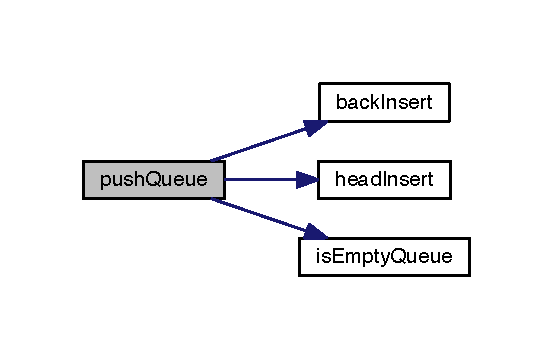
\includegraphics[width=265pt]{d4/da4/class_queue_a0012fa831aa1529e5ed3a6610b733423_cgraph}
\end{center}
\end{figure}




Her er kalder-\/grafen for denne funktion\+:
\nopagebreak
\begin{figure}[H]
\begin{center}
\leavevmode
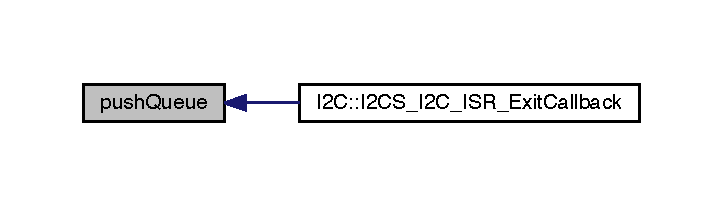
\includegraphics[width=347pt]{d4/da4/class_queue_a0012fa831aa1529e5ed3a6610b733423_icgraph}
\end{center}
\end{figure}


\index{Queue@{Queue}!queue\+\_\+init@{queue\+\_\+init}}
\index{queue\+\_\+init@{queue\+\_\+init}!Queue@{Queue}}
\paragraph[{\texorpdfstring{queue\+\_\+init(uint8 queue\+Max\+Size)}{queue_init(uint8 queueMaxSize)}}]{\setlength{\rightskip}{0pt plus 5cm}void queue\+\_\+init (
\begin{DoxyParamCaption}
\item[{uint8}]{queue\+Max\+Size}
\end{DoxyParamCaption}
)}\hypertarget{class_queue_a4e0a3758d721506e7729f4d074a280ff}{}\label{class_queue_a4e0a3758d721506e7729f4d074a280ff}


Initialiser \hyperlink{class_queue}{Queue} modulet. 

Initailiser køen med den ønsket max størelse.

\begin{DoxyAuthor}{Forfatter}
Jeppe Stærk Antonsen (\href{mailto:201271201@uni.au.dk}{\tt 201271201@uni.\+au.\+dk}) 
\end{DoxyAuthor}


Defineret på linje 89 i filen queue.\+c.



Indeholder referencer til Node\+::next\+\_\+.



Refereret til af main().


\begin{DoxyCode}
90 \{
91   \hyperlink{class_queue_aa48f05218d0a78402821c8aa9bdad06a}{frontOfQueuePtr\_} = NULL;
92   \hyperlink{class_queue_aa48f05218d0a78402821c8aa9bdad06a}{frontOfQueuePtr\_}->\hyperlink{queue_8c_a882bca6dea645e11ca1df6bc3c30ac42}{next\_} = NULL;
93   \hyperlink{class_queue_a225d2c9ad4e83d6da443e99b8869a51c}{backOfQueuePtr\_} = NULL;
94   \hyperlink{class_queue_a225d2c9ad4e83d6da443e99b8869a51c}{backOfQueuePtr\_}->\hyperlink{queue_8c_a882bca6dea645e11ca1df6bc3c30ac42}{next\_} = NULL;
95   \hyperlink{class_queue_acb6b6e88c9e4d12839594b31e6ff7c5a}{queueMax\_} = queueMaxSize;
96   \hyperlink{class_queue_ad260f9ccca00e80d161bbf3e70c3ffa6}{queueCount\_} = 0;
97 \}
\end{DoxyCode}


Her er kalder-\/grafen for denne funktion\+:
\nopagebreak
\begin{figure}[H]
\begin{center}
\leavevmode
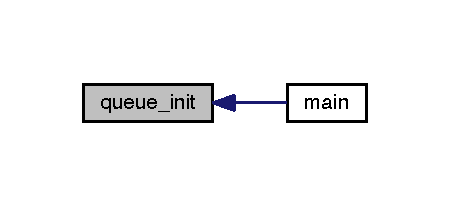
\includegraphics[width=216pt]{d4/da4/class_queue_a4e0a3758d721506e7729f4d074a280ff_icgraph}
\end{center}
\end{figure}




\subsubsection{Felt-\/dokumentation}
\index{Queue@{Queue}!back\+Of\+Queue\+Ptr\+\_\+@{back\+Of\+Queue\+Ptr\+\_\+}}
\index{back\+Of\+Queue\+Ptr\+\_\+@{back\+Of\+Queue\+Ptr\+\_\+}!Queue@{Queue}}
\paragraph[{\texorpdfstring{back\+Of\+Queue\+Ptr\+\_\+}{backOfQueuePtr_}}]{\setlength{\rightskip}{0pt plus 5cm}struct {\bf Node}$\ast$ back\+Of\+Queue\+Ptr\+\_\+\hspace{0.3cm}{\ttfamily [static]}, {\ttfamily [private]}}\hypertarget{class_queue_a225d2c9ad4e83d6da443e99b8869a51c}{}\label{class_queue_a225d2c9ad4e83d6da443e99b8869a51c}


Pointer til bagerste element i køen. 

En \hyperlink{queue_8c_db/d8b/struct_node}{Node} pointer der indeholder adressen på det bagerste elementet i køen.

\begin{DoxyAuthor}{Forfatter}
Jeppe Stærk Antonsen (\href{mailto:201271201@uni.au.dk}{\tt 201271201@uni.\+au.\+dk}) 
\end{DoxyAuthor}


Defineret på linje 48 i filen queue.\+c.

\index{Queue@{Queue}!front\+Of\+Queue\+Ptr\+\_\+@{front\+Of\+Queue\+Ptr\+\_\+}}
\index{front\+Of\+Queue\+Ptr\+\_\+@{front\+Of\+Queue\+Ptr\+\_\+}!Queue@{Queue}}
\paragraph[{\texorpdfstring{front\+Of\+Queue\+Ptr\+\_\+}{frontOfQueuePtr_}}]{\setlength{\rightskip}{0pt plus 5cm}struct {\bf Node}$\ast$ front\+Of\+Queue\+Ptr\+\_\+\hspace{0.3cm}{\ttfamily [static]}, {\ttfamily [private]}}\hypertarget{class_queue_aa48f05218d0a78402821c8aa9bdad06a}{}\label{class_queue_aa48f05218d0a78402821c8aa9bdad06a}


Pointer til foreste element i køen. 

En \hyperlink{queue_8c_db/d8b/struct_node}{Node} pointer der indeholder adressen på det foreste elementet i køen.

\begin{DoxyAuthor}{Forfatter}
Jeppe Stærk Antonsen (\href{mailto:201271201@uni.au.dk}{\tt 201271201@uni.\+au.\+dk}) 
\end{DoxyAuthor}


Defineret på linje 39 i filen queue.\+c.

\index{Queue@{Queue}!queue\+Count\+\_\+@{queue\+Count\+\_\+}}
\index{queue\+Count\+\_\+@{queue\+Count\+\_\+}!Queue@{Queue}}
\paragraph[{\texorpdfstring{queue\+Count\+\_\+}{queueCount_}}]{\setlength{\rightskip}{0pt plus 5cm}uint8 queue\+Count\+\_\+\hspace{0.3cm}{\ttfamily [static]}, {\ttfamily [private]}}\hypertarget{class_queue_ad260f9ccca00e80d161bbf3e70c3ffa6}{}\label{class_queue_ad260f9ccca00e80d161bbf3e70c3ffa6}


Kø element tæller. 

Bruges til at tælle hvor mange elementer der er i køen.

\begin{DoxyAuthor}{Forfatter}
Jeppe Stærk Antonsen (\href{mailto:201271201@uni.au.dk}{\tt 201271201@uni.\+au.\+dk}) 
\end{DoxyAuthor}


Defineret på linje 66 i filen queue.\+c.

\index{Queue@{Queue}!queue\+Max\+\_\+@{queue\+Max\+\_\+}}
\index{queue\+Max\+\_\+@{queue\+Max\+\_\+}!Queue@{Queue}}
\paragraph[{\texorpdfstring{queue\+Max\+\_\+}{queueMax_}}]{\setlength{\rightskip}{0pt plus 5cm}uint8 queue\+Max\+\_\+\hspace{0.3cm}{\ttfamily [static]}, {\ttfamily [private]}}\hypertarget{class_queue_acb6b6e88c9e4d12839594b31e6ff7c5a}{}\label{class_queue_acb6b6e88c9e4d12839594b31e6ff7c5a}


Køens max. 

Laver ved initialisering der ønsket antal for max elementer i køen

\begin{DoxyAuthor}{Forfatter}
Jeppe Stærk Antonsen (\href{mailto:201271201@uni.au.dk}{\tt 201271201@uni.\+au.\+dk}) 
\end{DoxyAuthor}


Defineret på linje 57 i filen queue.\+c.



Dokumentationen for denne klasse blev genereret ud fra filerne\+:\begin{DoxyCompactItemize}
\item 
\hyperlink{queue_8h}{queue.\+h}\item 
\hyperlink{queue_8c}{queue.\+c}\end{DoxyCompactItemize}

\hypertarget{class_z}{}\subsection{Z Klasse-\/reference}
\label{class_z}\index{Z@{Z}}


\hyperlink{class_z}{Z} class.  




{\ttfamily \#include $<$z.\+h$>$}



Samarbejdsdiagram for Z\+:
\nopagebreak
\begin{figure}[H]
\begin{center}
\leavevmode
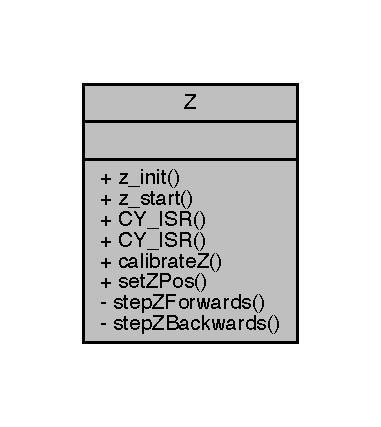
\includegraphics[width=183pt]{d5/d58/class_z__coll__graph}
\end{center}
\end{figure}
\subsubsection*{Offentlige metoder}
\begin{DoxyCompactItemize}
\item 
void \hyperlink{class_z_ac6bb96bf63bd2cae7c7bcc2f6b422b0c}{z\+\_\+init} ()
\begin{DoxyCompactList}\small\item\em Initialiser \hyperlink{class_z}{Z} modulet. \end{DoxyCompactList}\item 
void \hyperlink{class_z_affabc649bbf2e5dbeb475777391513d7}{z\+\_\+start} ()
\begin{DoxyCompactList}\small\item\em Starter \hyperlink{class_z}{Z} modulet. \end{DoxyCompactList}\item 
\hyperlink{class_z_a8171ad8aabdbfed5d19fbda53c9d28a9}{C\+Y\+\_\+\+I\+SR} (isr\+\_\+Z)
\begin{DoxyCompactList}\small\item\em Afvikler \char`\"{}\+Interrupt\char`\"{} fra \hyperlink{class_z}{Z}. \end{DoxyCompactList}\item 
\hyperlink{class_z_a55737cff8ccce80876ed873475f484ba}{C\+Y\+\_\+\+I\+SR} (isr\+\_\+S)
\begin{DoxyCompactList}\small\item\em Afvikler \char`\"{}\+Interrupt\char`\"{} fra \hyperlink{class_z}{Z}. \end{DoxyCompactList}\item 
void \hyperlink{class_z_a75e9200c2d48803f4bb723bd1fea24ea}{calibrateZ} ()
\begin{DoxyCompactList}\small\item\em Kalibrere \hyperlink{class_z}{Z}. \end{DoxyCompactList}\item 
void \hyperlink{class_z_a32c07d919fae10a36ead3ac6766f7355}{set\+Z\+Pos} (uint8 z\+Val)
\begin{DoxyCompactList}\small\item\em Sætter ny \hyperlink{class_z}{Z} position. \end{DoxyCompactList}\end{DoxyCompactItemize}
\subsubsection*{Private metoder}
\begin{DoxyCompactItemize}
\item 
void \hyperlink{class_z_aeac8c479305ae54b347729e4ff279d44}{step\+Z\+Forwards} ()
\begin{DoxyCompactList}\small\item\em Køre \hyperlink{class_z}{Z} motor et step frem. \end{DoxyCompactList}\item 
void \hyperlink{class_z_ad16ddc5261a237fc03c8a4b30571c528}{step\+Z\+Backwards} ()
\begin{DoxyCompactList}\small\item\em Køre \hyperlink{class_z}{Z} motor et step tilbage. \end{DoxyCompactList}\end{DoxyCompactItemize}


\subsubsection{Detaljeret beskrivelse}
\hyperlink{class_z}{Z} class. 

Styre \hyperlink{class_z}{Z} modulets funktioner. \begin{DoxyAuthor}{Forfatter}
Casper Dieu Le (\href{mailto:201370338@uni.au.dk}{\tt 201370338@uni.\+au.\+dk}) 

Kasper Hinkler Uldbjerg (\href{mailto:201370281@uni.au.dk}{\tt 201370281@uni.\+au.\+dk}) 

Jeppe Stærk Antonsen (\href{mailto:201271201@uni.au.dk}{\tt 201271201@uni.\+au.\+dk}) 
\end{DoxyAuthor}


\subsubsection{Dokumentation af medlemsfunktioner}
\index{Z@{Z}!calibrateZ@{calibrateZ}}
\index{calibrateZ@{calibrateZ}!Z@{Z}}
\paragraph[{\texorpdfstring{calibrate\+Z()}{calibrateZ()}}]{\setlength{\rightskip}{0pt plus 5cm}void calibrateZ (
\begin{DoxyParamCaption}
\item[{void}]{}
\end{DoxyParamCaption}
)}\hypertarget{class_z_a75e9200c2d48803f4bb723bd1fea24ea}{}\label{class_z_a75e9200c2d48803f4bb723bd1fea24ea}


Kalibrere \hyperlink{class_z}{Z}. 

Metoden kalibrerer \hyperlink{class_z}{Z} og sætter en ny max værdi for \hyperlink{class_z}{Z}.

\begin{DoxyAuthor}{Forfatter}
Casper Dieu Le (\href{mailto:201370338@uni.au.dk}{\tt 201370338@uni.\+au.\+dk}) 

Kasper Hinkler Uldbjerg (\href{mailto:201370281@uni.au.dk}{\tt 201370281@uni.\+au.\+dk}) 

Jeppe Stærk Antonsen (\href{mailto:201271201@uni.au.dk}{\tt 201271201@uni.\+au.\+dk}) 
\end{DoxyAuthor}


Defineret på linje 137 i filen z.\+c.



Indeholder referencer til Data\+Z\+::calibratedZ, dataZ, interrupt\+Steps, Data\+Z\+::interruptZ, L\+E\+D\+::set\+Led(), step\+Z\+Backwards(), step\+Z\+Forwards(), Data\+Z\+::z\+Flag, Data\+Z\+::z\+Max og Data\+Z\+::z\+Pos.



Refereret til af Handler\+::handler(), main() og set\+Z\+Pos().


\begin{DoxyCode}
138 \{
139   DEBUG\_PutString(\textcolor{stringliteral}{"Z calibrate pre-zMax: "});
140   DEBUG\_PutHexInt(\hyperlink{data_8h_ace1aa5b973b9358f7236c0c9deca9370}{dataZ}.\hyperlink{data_8h_a73591b48f5bcc31997bc92dc465d6696}{zMax});
141   DEBUG\_PutCRLF();
142   
143   \hyperlink{data_8h_ace1aa5b973b9358f7236c0c9deca9370}{dataZ}.\hyperlink{data_8h_ae018a4b3f38c25bf309a70bfa3c2b47b}{calibratedZ} = 0;
144   \hyperlink{data_8h_ace1aa5b973b9358f7236c0c9deca9370}{dataZ}.\hyperlink{data_8h_ac9b1acf86d4646bdf8e9f338aedb56a2}{zFlag} = 1;
145   \hyperlink{data_8h_ace1aa5b973b9358f7236c0c9deca9370}{dataZ}.\hyperlink{data_8h_a73591b48f5bcc31997bc92dc465d6696}{zMax} = 0;
146   
147   DEBUG\_PutString(\textcolor{stringliteral}{"Going forwards to max"});
148   \textcolor{keywordflow}{while}(\hyperlink{data_8h_ace1aa5b973b9358f7236c0c9deca9370}{dataZ}.\hyperlink{data_8h_ad31cb1c3240ac1f76fc3faa902b49c24}{interruptZ} == 0 && \hyperlink{data_8h_ace1aa5b973b9358f7236c0c9deca9370}{dataZ}.\hyperlink{data_8h_ac9b1acf86d4646bdf8e9f338aedb56a2}{zFlag} == 1)
149   \{
150     DEBUG\_PutString(\textcolor{stringliteral}{"."});
151     \hyperlink{led_8h_a1d8e725e3829da99c1d027ba0a2ce57a}{setLed}(1,0,0,0);
152     \hyperlink{class_z_aeac8c479305ae54b347729e4ff279d44}{stepZForwards}();
153   \}
154   \hyperlink{data_8h_ace1aa5b973b9358f7236c0c9deca9370}{dataZ}.\hyperlink{data_8h_ad31cb1c3240ac1f76fc3faa902b49c24}{interruptZ} = 0;
155   
156   DEBUG\_PutString(\textcolor{stringliteral}{"done"});
157   DEBUG\_PutCRLF();
158   
159   DEBUG\_PutString(\textcolor{stringliteral}{"Going backwards to zero"});
160   \textcolor{keywordflow}{while}(\hyperlink{data_8h_ace1aa5b973b9358f7236c0c9deca9370}{dataZ}.\hyperlink{data_8h_ad31cb1c3240ac1f76fc3faa902b49c24}{interruptZ} == 0 && \hyperlink{data_8h_ace1aa5b973b9358f7236c0c9deca9370}{dataZ}.\hyperlink{data_8h_ac9b1acf86d4646bdf8e9f338aedb56a2}{zFlag} == 0)
161   \{
162     DEBUG\_PutString(\textcolor{stringliteral}{"."});
163     \hyperlink{led_8h_a1d8e725e3829da99c1d027ba0a2ce57a}{setLed}(1,0,0,0);
164     \hyperlink{class_z_ad16ddc5261a237fc03c8a4b30571c528}{stepZBackwards}();
165     \hyperlink{data_8h_ace1aa5b973b9358f7236c0c9deca9370}{dataZ}.\hyperlink{data_8h_a73591b48f5bcc31997bc92dc465d6696}{zMax}++;
166   \}
167   DEBUG\_PutString(\textcolor{stringliteral}{"done"});
168 
169   \hyperlink{led_8h_a1d8e725e3829da99c1d027ba0a2ce57a}{setLed}(0,0,0,0);
170   
171   \hyperlink{data_8h_ace1aa5b973b9358f7236c0c9deca9370}{dataZ}.\hyperlink{data_8h_aafb6592f063176df6830ef1f1e29ae72}{zPos} = 0;
172   \hyperlink{data_8h_ace1aa5b973b9358f7236c0c9deca9370}{dataZ}.\hyperlink{data_8h_a73591b48f5bcc31997bc92dc465d6696}{zMax} = \hyperlink{data_8h_ace1aa5b973b9358f7236c0c9deca9370}{dataZ}.\hyperlink{data_8h_a73591b48f5bcc31997bc92dc465d6696}{zMax} - \hyperlink{z_8h_a319d8f8cbb816fc1ca2306587712b0b7}{interruptSteps};
173   
174   DEBUG\_PutString(\textcolor{stringliteral}{" post-zMax: "});
175   DEBUG\_PutHexInt(\hyperlink{data_8h_ace1aa5b973b9358f7236c0c9deca9370}{dataZ}.\hyperlink{data_8h_a73591b48f5bcc31997bc92dc465d6696}{zMax});
176   DEBUG\_PutString(\textcolor{stringliteral}{" new xPos: "});
177   DEBUG\_PutHexInt(\hyperlink{data_8h_ace1aa5b973b9358f7236c0c9deca9370}{dataZ}.\hyperlink{data_8h_aafb6592f063176df6830ef1f1e29ae72}{zPos});
178   DEBUG\_PutCRLF();
179   DEBUG\_PutCRLF();
180   
181   \hyperlink{data_8h_ace1aa5b973b9358f7236c0c9deca9370}{dataZ}.\hyperlink{data_8h_ae018a4b3f38c25bf309a70bfa3c2b47b}{calibratedZ} = 1;
182   \hyperlink{data_8h_ace1aa5b973b9358f7236c0c9deca9370}{dataZ}.\hyperlink{data_8h_ad31cb1c3240ac1f76fc3faa902b49c24}{interruptZ} = 0;
183 \}
\end{DoxyCode}


Her er kald-\/grafen for denne funktion\+:
\nopagebreak
\begin{figure}[H]
\begin{center}
\leavevmode
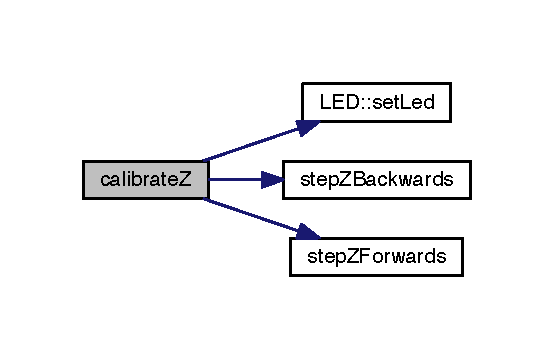
\includegraphics[width=266pt]{d7/d97/class_z_a75e9200c2d48803f4bb723bd1fea24ea_cgraph}
\end{center}
\end{figure}




Her er kalder-\/grafen for denne funktion\+:
\nopagebreak
\begin{figure}[H]
\begin{center}
\leavevmode
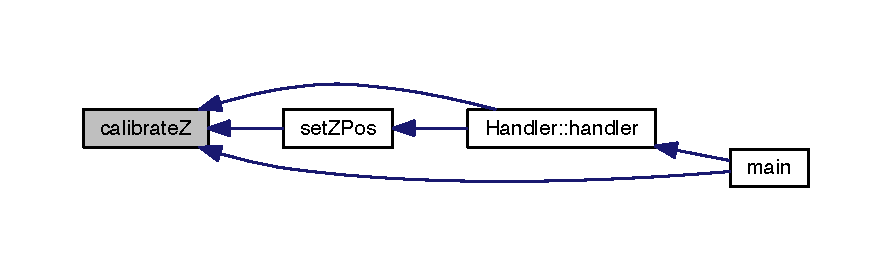
\includegraphics[width=350pt]{d7/d97/class_z_a75e9200c2d48803f4bb723bd1fea24ea_icgraph}
\end{center}
\end{figure}


\index{Z@{Z}!C\+Y\+\_\+\+I\+SR@{C\+Y\+\_\+\+I\+SR}}
\index{C\+Y\+\_\+\+I\+SR@{C\+Y\+\_\+\+I\+SR}!Z@{Z}}
\paragraph[{\texorpdfstring{C\+Y\+\_\+\+I\+S\+R(isr\+\_\+\+Z)}{CY_ISR(isr_Z)}}]{\setlength{\rightskip}{0pt plus 5cm}C\+Y\+\_\+\+I\+SR (
\begin{DoxyParamCaption}
\item[{isr\+\_\+Z}]{}
\end{DoxyParamCaption}
)}\hypertarget{class_z_a8171ad8aabdbfed5d19fbda53c9d28a9}{}\label{class_z_a8171ad8aabdbfed5d19fbda53c9d28a9}


Afvikler \char`\"{}\+Interrupt\char`\"{} fra \hyperlink{class_z}{Z}. 

En \char`\"{}\+Interrupt Service Routine(\+I\+S\+R)\char`\"{} for \hyperlink{class_z}{Z} der aktiveres ved interrupt fra \hyperlink{class_z}{Z} modulet.

\begin{DoxyAuthor}{Forfatter}
Casper Dieu Le (\href{mailto:201370338@uni.au.dk}{\tt 201370338@uni.\+au.\+dk}) 

Kasper Hinkler Uldbjerg (\href{mailto:201370281@uni.au.dk}{\tt 201370281@uni.\+au.\+dk}) 

Jeppe Stærk Antonsen (\href{mailto:201271201@uni.au.dk}{\tt 201271201@uni.\+au.\+dk}) 
\end{DoxyAuthor}


Defineret på linje 75 i filen z.\+c.



Indeholder referencer til dataZ, interrupt\+Steps, Data\+Z\+::interruptZ, L\+E\+D\+::set\+Led(), step\+Z\+Forwards() og Data\+Z\+::z\+Flag.


\begin{DoxyCode}
76 \{
77   DEBUG\_PutString(\textcolor{stringliteral}{"Interrupt Z"});
78   DEBUG\_PutCRLF();
79   interrupt\_Z\_Disable();
80   
81   uint32 i;
82   
83   \hyperlink{data_8h_ace1aa5b973b9358f7236c0c9deca9370}{dataZ}.\hyperlink{data_8h_ad31cb1c3240ac1f76fc3faa902b49c24}{interruptZ} = 1;
84 
85   \hyperlink{led_8h_a1d8e725e3829da99c1d027ba0a2ce57a}{setLed}(0,0,1,0);
86   \textcolor{keywordflow}{for}(i = 0; i < \hyperlink{z_8h_a319d8f8cbb816fc1ca2306587712b0b7}{interruptSteps}; i++)
87   \{
88     \hyperlink{class_z_aeac8c479305ae54b347729e4ff279d44}{stepZForwards}();
89   \}
90   \hyperlink{data_8h_ace1aa5b973b9358f7236c0c9deca9370}{dataZ}.\hyperlink{data_8h_ac9b1acf86d4646bdf8e9f338aedb56a2}{zFlag} = 1;
91   \hyperlink{led_8h_a1d8e725e3829da99c1d027ba0a2ce57a}{setLed}(0,0,0,0);
92   
93   interrupt\_Z\_ClearPending();
94   interrupt\_Z\_Enable();
95 \}
\end{DoxyCode}


Her er kald-\/grafen for denne funktion\+:
\nopagebreak
\begin{figure}[H]
\begin{center}
\leavevmode
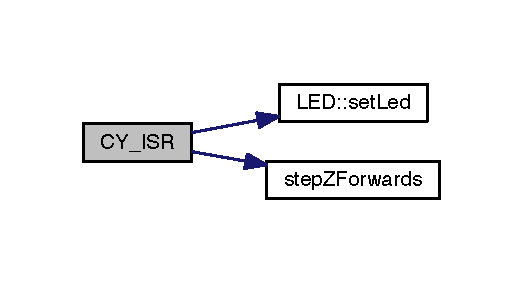
\includegraphics[width=251pt]{d7/d97/class_z_a8171ad8aabdbfed5d19fbda53c9d28a9_cgraph}
\end{center}
\end{figure}


\index{Z@{Z}!C\+Y\+\_\+\+I\+SR@{C\+Y\+\_\+\+I\+SR}}
\index{C\+Y\+\_\+\+I\+SR@{C\+Y\+\_\+\+I\+SR}!Z@{Z}}
\paragraph[{\texorpdfstring{C\+Y\+\_\+\+I\+S\+R(isr\+\_\+\+S)}{CY_ISR(isr_S)}}]{\setlength{\rightskip}{0pt plus 5cm}C\+Y\+\_\+\+I\+SR (
\begin{DoxyParamCaption}
\item[{isr\+\_\+S}]{}
\end{DoxyParamCaption}
)}\hypertarget{class_z_a55737cff8ccce80876ed873475f484ba}{}\label{class_z_a55737cff8ccce80876ed873475f484ba}


Afvikler \char`\"{}\+Interrupt\char`\"{} fra \hyperlink{class_z}{Z}. 

En \char`\"{}\+Interrupt Service Routine(\+I\+S\+R)\char`\"{} for \hyperlink{class_z}{Z} der aktiveres ved interrupt fra \hyperlink{class_z}{Z} modulet.

\begin{DoxyAuthor}{Forfatter}
Casper Dieu Le (\href{mailto:201370338@uni.au.dk}{\tt 201370338@uni.\+au.\+dk}) 

Kasper Hinkler Uldbjerg (\href{mailto:201370281@uni.au.dk}{\tt 201370281@uni.\+au.\+dk}) 

Jeppe Stærk Antonsen (\href{mailto:201271201@uni.au.dk}{\tt 201271201@uni.\+au.\+dk}) 
\end{DoxyAuthor}


Defineret på linje 106 i filen z.\+c.



Indeholder referencer til dataZ, interrupt\+Steps, Data\+Z\+::interruptZ, L\+E\+D\+::set\+Led(), step\+Z\+Backwards() og Data\+Z\+::z\+Flag.


\begin{DoxyCode}
107 \{
108   DEBUG\_PutString(\textcolor{stringliteral}{"Interrupt S"});
109   DEBUG\_PutCRLF();
110   interrupt\_S\_Disable();
111   
112   uint32 i;
113   
114   \hyperlink{data_8h_ace1aa5b973b9358f7236c0c9deca9370}{dataZ}.\hyperlink{data_8h_ad31cb1c3240ac1f76fc3faa902b49c24}{interruptZ} = 1;
115   
116   \hyperlink{led_8h_a1d8e725e3829da99c1d027ba0a2ce57a}{setLed}(0,0,1,0);
117   \textcolor{keywordflow}{for}(i = 0; i < \hyperlink{z_8h_a319d8f8cbb816fc1ca2306587712b0b7}{interruptSteps}; i++)
118   \{
119     \hyperlink{class_z_ad16ddc5261a237fc03c8a4b30571c528}{stepZBackwards}();
120   \}
121   \hyperlink{data_8h_ace1aa5b973b9358f7236c0c9deca9370}{dataZ}.\hyperlink{data_8h_ac9b1acf86d4646bdf8e9f338aedb56a2}{zFlag} = 0;
122   \hyperlink{led_8h_a1d8e725e3829da99c1d027ba0a2ce57a}{setLed}(0,0,0,0);
123   
124   interrupt\_S\_ClearPending();
125   interrupt\_S\_Enable();
126 \}
\end{DoxyCode}


Her er kald-\/grafen for denne funktion\+:
\nopagebreak
\begin{figure}[H]
\begin{center}
\leavevmode
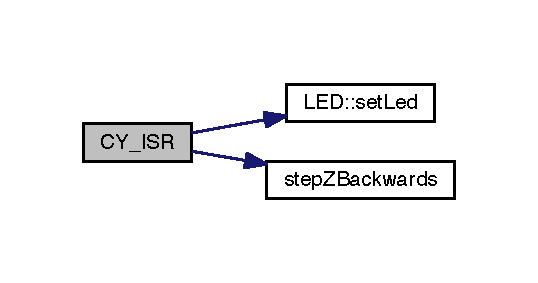
\includegraphics[width=258pt]{d7/d97/class_z_a55737cff8ccce80876ed873475f484ba_cgraph}
\end{center}
\end{figure}


\index{Z@{Z}!set\+Z\+Pos@{set\+Z\+Pos}}
\index{set\+Z\+Pos@{set\+Z\+Pos}!Z@{Z}}
\paragraph[{\texorpdfstring{set\+Z\+Pos(uint8 z\+Val)}{setZPos(uint8 zVal)}}]{\setlength{\rightskip}{0pt plus 5cm}void set\+Z\+Pos (
\begin{DoxyParamCaption}
\item[{uint8}]{z\+Val}
\end{DoxyParamCaption}
)}\hypertarget{class_z_a32c07d919fae10a36ead3ac6766f7355}{}\label{class_z_a32c07d919fae10a36ead3ac6766f7355}


Sætter ny \hyperlink{class_z}{Z} position. 

Ud fra den modtaget værdi udregnes antal step og vej til den ønsket destination. 
\begin{DoxyParams}[1]{Parametre}
\mbox{\tt in}  & {\em z\+Val} & Værdi for position.\\
\hline
\end{DoxyParams}
\begin{DoxyAuthor}{Forfatter}
Casper Dieu Le (\href{mailto:201370338@uni.au.dk}{\tt 201370338@uni.\+au.\+dk}) 

Kasper Hinkler Uldbjerg (\href{mailto:201370281@uni.au.dk}{\tt 201370281@uni.\+au.\+dk}) 

Jeppe Stærk Antonsen (\href{mailto:201271201@uni.au.dk}{\tt 201271201@uni.\+au.\+dk}) 
\end{DoxyAuthor}


Defineret på linje 195 i filen z.\+c.



Indeholder referencer til Data\+Z\+::calibratedZ, calibrate\+Z(), dataZ, Data\+Z\+::interruptZ, Data\+Z\+::isr\+StopZ, resolution, L\+E\+D\+::set\+Led(), step\+Z\+Backwards(), step\+Z\+Forwards(), Data\+Z\+::z\+Flag, Data\+Z\+::z\+Max og Data\+Z\+::z\+Pos.



Refereret til af Handler\+::handler().


\begin{DoxyCode}
196 \{
197   uint32 i;
198   uint32 zDes = 0;
199   uint32 zSteps = 0;
200   
201   \hyperlink{data_8h_ace1aa5b973b9358f7236c0c9deca9370}{dataZ}.\hyperlink{data_8h_ae55ff8378d0a07b118000a98b273141f}{isrStopZ} = 0;
202   
203   \textcolor{keywordflow}{if}(\hyperlink{data_8h_ace1aa5b973b9358f7236c0c9deca9370}{dataZ}.\hyperlink{data_8h_ae018a4b3f38c25bf309a70bfa3c2b47b}{calibratedZ} == 1)
204   \{
205     zDes = zVal * \hyperlink{data_8h_ace1aa5b973b9358f7236c0c9deca9370}{dataZ}.\hyperlink{data_8h_a73591b48f5bcc31997bc92dc465d6696}{zMax} / \hyperlink{z_8h_a518902ce4d6b0c41b04e9fcd3c648916}{resolution};
206     
207     DEBUG\_PutString(\textcolor{stringliteral}{"Z set value: "});
208     DEBUG\_PutHexInt(zVal);
209     DEBUG\_PutString(\textcolor{stringliteral}{" pre-zPos: "});
210     DEBUG\_PutHexInt(\hyperlink{data_8h_ace1aa5b973b9358f7236c0c9deca9370}{dataZ}.\hyperlink{data_8h_aafb6592f063176df6830ef1f1e29ae72}{zPos});
211     DEBUG\_PutString(\textcolor{stringliteral}{" zDes: "});
212     DEBUG\_PutHexInt(zDes);
213     
214     \textcolor{keywordflow}{if}(zDes > \hyperlink{data_8h_ace1aa5b973b9358f7236c0c9deca9370}{dataZ}.\hyperlink{data_8h_aafb6592f063176df6830ef1f1e29ae72}{zPos})
215     \{
216       \hyperlink{led_8h_a1d8e725e3829da99c1d027ba0a2ce57a}{setLed}(0,1,0,0);
217       \hyperlink{data_8h_ace1aa5b973b9358f7236c0c9deca9370}{dataZ}.\hyperlink{data_8h_ad31cb1c3240ac1f76fc3faa902b49c24}{interruptZ} = 0;
218       \hyperlink{data_8h_ace1aa5b973b9358f7236c0c9deca9370}{dataZ}.\hyperlink{data_8h_ac9b1acf86d4646bdf8e9f338aedb56a2}{zFlag} = 1;
219       zSteps = zDes - \hyperlink{data_8h_ace1aa5b973b9358f7236c0c9deca9370}{dataZ}.\hyperlink{data_8h_aafb6592f063176df6830ef1f1e29ae72}{zPos};
220       
221       DEBUG\_PutString(\textcolor{stringliteral}{" going forwards steps: "});
222       DEBUG\_PutHexInt(zSteps);
223       \textcolor{keywordflow}{for}(i = 0; i < zSteps  && \hyperlink{data_8h_ace1aa5b973b9358f7236c0c9deca9370}{dataZ}.\hyperlink{data_8h_ae55ff8378d0a07b118000a98b273141f}{isrStopZ} == 0 && \hyperlink{data_8h_ace1aa5b973b9358f7236c0c9deca9370}{dataZ}.
      \hyperlink{data_8h_ad31cb1c3240ac1f76fc3faa902b49c24}{interruptZ} == 0 && \hyperlink{data_8h_ace1aa5b973b9358f7236c0c9deca9370}{dataZ}.\hyperlink{data_8h_ac9b1acf86d4646bdf8e9f338aedb56a2}{zFlag} == 1; i++)
224       \{
225         DEBUG\_PutString(\textcolor{stringliteral}{"."});
226         \hyperlink{class_z_aeac8c479305ae54b347729e4ff279d44}{stepZForwards}();
227         \hyperlink{data_8h_ace1aa5b973b9358f7236c0c9deca9370}{dataZ}.\hyperlink{data_8h_aafb6592f063176df6830ef1f1e29ae72}{zPos}++;
228       \}
229       DEBUG\_PutString(\textcolor{stringliteral}{"done"});
230       
231       \textcolor{keywordflow}{if}(\hyperlink{data_8h_ace1aa5b973b9358f7236c0c9deca9370}{dataZ}.\hyperlink{data_8h_ad31cb1c3240ac1f76fc3faa902b49c24}{interruptZ} == 1)
232       \{
233         \hyperlink{data_8h_ace1aa5b973b9358f7236c0c9deca9370}{dataZ}.\hyperlink{data_8h_aafb6592f063176df6830ef1f1e29ae72}{zPos} = \hyperlink{data_8h_ace1aa5b973b9358f7236c0c9deca9370}{dataZ}.\hyperlink{data_8h_a73591b48f5bcc31997bc92dc465d6696}{zMax};
234       \}
235       DEBUG\_PutString(\textcolor{stringliteral}{" new-zPos: "});
236       DEBUG\_PutHexInt(\hyperlink{data_8h_ace1aa5b973b9358f7236c0c9deca9370}{dataZ}.\hyperlink{data_8h_aafb6592f063176df6830ef1f1e29ae72}{zPos});
237       DEBUG\_PutCRLF();
238       DEBUG\_PutCRLF();
239       
240       \hyperlink{led_8h_a1d8e725e3829da99c1d027ba0a2ce57a}{setLed}(0,0,0,0);
241     \}
242     \textcolor{keywordflow}{else} \textcolor{keywordflow}{if}(zDes < \hyperlink{data_8h_ace1aa5b973b9358f7236c0c9deca9370}{dataZ}.\hyperlink{data_8h_aafb6592f063176df6830ef1f1e29ae72}{zPos})
243     \{
244       \hyperlink{led_8h_a1d8e725e3829da99c1d027ba0a2ce57a}{setLed}(0,1,0,0);
245       
246       \hyperlink{data_8h_ace1aa5b973b9358f7236c0c9deca9370}{dataZ}.\hyperlink{data_8h_ad31cb1c3240ac1f76fc3faa902b49c24}{interruptZ} = 0;
247       \hyperlink{data_8h_ace1aa5b973b9358f7236c0c9deca9370}{dataZ}.\hyperlink{data_8h_ac9b1acf86d4646bdf8e9f338aedb56a2}{zFlag} = 0;
248       zSteps = \hyperlink{data_8h_ace1aa5b973b9358f7236c0c9deca9370}{dataZ}.\hyperlink{data_8h_aafb6592f063176df6830ef1f1e29ae72}{zPos} - zDes;
249       
250       DEBUG\_PutString(\textcolor{stringliteral}{" going backwards steps: "});
251       DEBUG\_PutHexInt(zSteps);
252       \textcolor{keywordflow}{for}(i = 0; i < zSteps && \hyperlink{data_8h_ace1aa5b973b9358f7236c0c9deca9370}{dataZ}.\hyperlink{data_8h_ae55ff8378d0a07b118000a98b273141f}{isrStopZ} == 0 && \hyperlink{data_8h_ace1aa5b973b9358f7236c0c9deca9370}{dataZ}.
      \hyperlink{data_8h_ad31cb1c3240ac1f76fc3faa902b49c24}{interruptZ} == 0 && \hyperlink{data_8h_ace1aa5b973b9358f7236c0c9deca9370}{dataZ}.\hyperlink{data_8h_ac9b1acf86d4646bdf8e9f338aedb56a2}{zFlag} == 0; i++)
253       \{
254         DEBUG\_PutString(\textcolor{stringliteral}{"."});
255         \hyperlink{class_z_ad16ddc5261a237fc03c8a4b30571c528}{stepZBackwards}();
256         \hyperlink{data_8h_ace1aa5b973b9358f7236c0c9deca9370}{dataZ}.\hyperlink{data_8h_aafb6592f063176df6830ef1f1e29ae72}{zPos}--;
257       \}
258       DEBUG\_PutString(\textcolor{stringliteral}{"done"});
259       \textcolor{keywordflow}{if}(\hyperlink{data_8h_ace1aa5b973b9358f7236c0c9deca9370}{dataZ}.\hyperlink{data_8h_ad31cb1c3240ac1f76fc3faa902b49c24}{interruptZ} == 1)
260       \{
261         \hyperlink{data_8h_ace1aa5b973b9358f7236c0c9deca9370}{dataZ}.\hyperlink{data_8h_aafb6592f063176df6830ef1f1e29ae72}{zPos} = 0;
262       \}
263       DEBUG\_PutString(\textcolor{stringliteral}{" new-zPos: "});
264       DEBUG\_PutHexInt(\hyperlink{data_8h_ace1aa5b973b9358f7236c0c9deca9370}{dataZ}.\hyperlink{data_8h_aafb6592f063176df6830ef1f1e29ae72}{zPos});
265       DEBUG\_PutCRLF();
266       DEBUG\_PutCRLF();
267       
268       \hyperlink{led_8h_a1d8e725e3829da99c1d027ba0a2ce57a}{setLed}(0,0,0,0);
269     \}
270   \}
271   \textcolor{keywordflow}{else}
272   \{
273     \hyperlink{class_z_a75e9200c2d48803f4bb723bd1fea24ea}{calibrateZ}();
274     \hyperlink{class_z_a32c07d919fae10a36ead3ac6766f7355}{setZPos}(zVal);
275   \}
276   \hyperlink{data_8h_ace1aa5b973b9358f7236c0c9deca9370}{dataZ}.\hyperlink{data_8h_ad31cb1c3240ac1f76fc3faa902b49c24}{interruptZ} = 0;
277 \}
\end{DoxyCode}


Her er kald-\/grafen for denne funktion\+:
\nopagebreak
\begin{figure}[H]
\begin{center}
\leavevmode
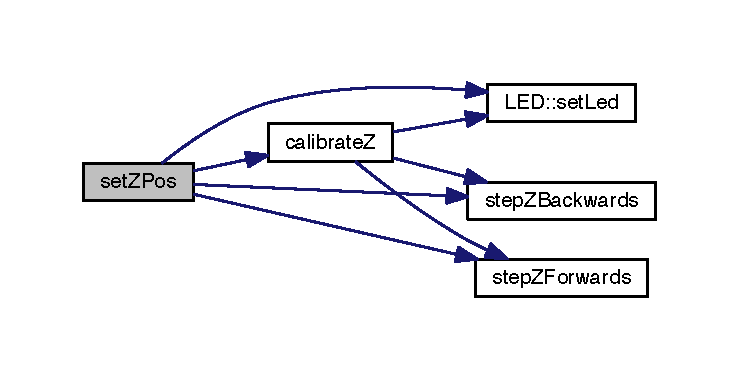
\includegraphics[width=350pt]{d7/d97/class_z_a32c07d919fae10a36ead3ac6766f7355_cgraph}
\end{center}
\end{figure}




Her er kalder-\/grafen for denne funktion\+:
\nopagebreak
\begin{figure}[H]
\begin{center}
\leavevmode
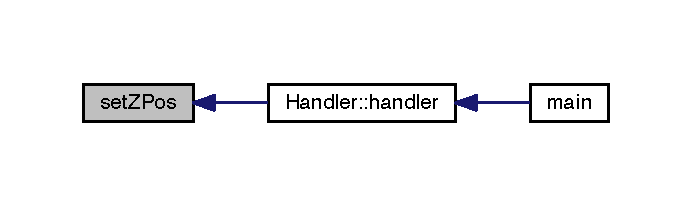
\includegraphics[width=332pt]{d7/d97/class_z_a32c07d919fae10a36ead3ac6766f7355_icgraph}
\end{center}
\end{figure}


\index{Z@{Z}!step\+Z\+Backwards@{step\+Z\+Backwards}}
\index{step\+Z\+Backwards@{step\+Z\+Backwards}!Z@{Z}}
\paragraph[{\texorpdfstring{step\+Z\+Backwards()}{stepZBackwards()}}]{\setlength{\rightskip}{0pt plus 5cm}void step\+Z\+Backwards (
\begin{DoxyParamCaption}
\item[{void}]{}
\end{DoxyParamCaption}
)\hspace{0.3cm}{\ttfamily [private]}}\hypertarget{class_z_ad16ddc5261a237fc03c8a4b30571c528}{}\label{class_z_ad16ddc5261a237fc03c8a4b30571c528}


Køre \hyperlink{class_z}{Z} motor et step tilbage. 

Køre \hyperlink{class_z}{Z} motoren et step tilbage.

\begin{DoxyAuthor}{Forfatter}
Casper Dieu Le (\href{mailto:201370338@uni.au.dk}{\tt 201370338@uni.\+au.\+dk}) 

Kasper Hinkler Uldbjerg (\href{mailto:201370281@uni.au.dk}{\tt 201370281@uni.\+au.\+dk}) 

Jeppe Stærk Antonsen (\href{mailto:201271201@uni.au.dk}{\tt 201271201@uni.\+au.\+dk}) 
\end{DoxyAuthor}


Defineret på linje 329 i filen z.\+c.



Indeholder referencer til step\+Delay.



Refereret til af calibrate\+Z(), C\+Y\+\_\+\+I\+S\+R(), set\+Z\+Pos() og z\+\_\+start().


\begin{DoxyCode}
330 \{
331   Pin\_1a\_Z\_Write(0);
332   Pin\_2a\_Z\_Write(0);
333   Pin\_1b\_Z\_Write(0);
334   Pin\_2b\_Z\_Write(1);
335   CyDelay(\hyperlink{z_8h_af24cf99e186a696ed4f58aff71d09249}{stepDelay});
336   
337   Pin\_1a\_Z\_Write(0);
338   Pin\_2a\_Z\_Write(0);
339   Pin\_1b\_Z\_Write(1);
340   Pin\_2b\_Z\_Write(0);
341   CyDelay(\hyperlink{z_8h_af24cf99e186a696ed4f58aff71d09249}{stepDelay});
342   
343   Pin\_1a\_Z\_Write(0);
344   Pin\_2a\_Z\_Write(1);
345   Pin\_1b\_Z\_Write(0);
346   Pin\_2b\_Z\_Write(0);
347   CyDelay(\hyperlink{z_8h_af24cf99e186a696ed4f58aff71d09249}{stepDelay});
348   
349   Pin\_1a\_Z\_Write(1);
350   Pin\_2a\_Z\_Write(0);
351   Pin\_1b\_Z\_Write(0);
352   Pin\_2b\_Z\_Write(0);
353   CyDelay(\hyperlink{z_8h_af24cf99e186a696ed4f58aff71d09249}{stepDelay});
354 \}
\end{DoxyCode}


Her er kalder-\/grafen for denne funktion\+:
\nopagebreak
\begin{figure}[H]
\begin{center}
\leavevmode
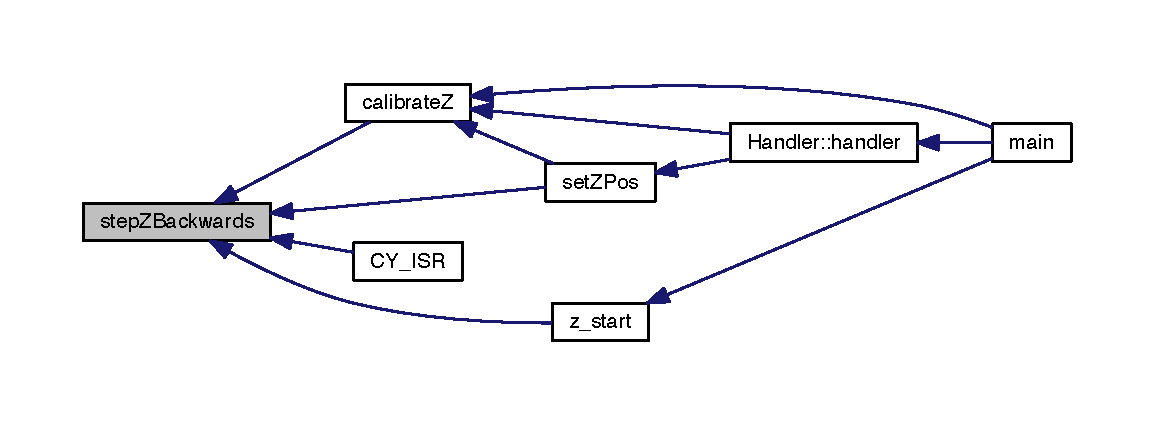
\includegraphics[width=350pt]{d7/d97/class_z_ad16ddc5261a237fc03c8a4b30571c528_icgraph}
\end{center}
\end{figure}


\index{Z@{Z}!step\+Z\+Forwards@{step\+Z\+Forwards}}
\index{step\+Z\+Forwards@{step\+Z\+Forwards}!Z@{Z}}
\paragraph[{\texorpdfstring{step\+Z\+Forwards()}{stepZForwards()}}]{\setlength{\rightskip}{0pt plus 5cm}void step\+Z\+Forwards (
\begin{DoxyParamCaption}
\item[{void}]{}
\end{DoxyParamCaption}
)\hspace{0.3cm}{\ttfamily [private]}}\hypertarget{class_z_aeac8c479305ae54b347729e4ff279d44}{}\label{class_z_aeac8c479305ae54b347729e4ff279d44}


Køre \hyperlink{class_z}{Z} motor et step frem. 

Køre \hyperlink{class_z}{Z} motoren et step fremad.

\begin{DoxyAuthor}{Forfatter}
Casper Dieu Le (\href{mailto:201370338@uni.au.dk}{\tt 201370338@uni.\+au.\+dk}) 

Kasper Hinkler Uldbjerg (\href{mailto:201370281@uni.au.dk}{\tt 201370281@uni.\+au.\+dk}) 

Jeppe Stærk Antonsen (\href{mailto:201271201@uni.au.dk}{\tt 201271201@uni.\+au.\+dk}) 
\end{DoxyAuthor}


Defineret på linje 293 i filen z.\+c.



Indeholder referencer til step\+Delay.



Refereret til af calibrate\+Z(), C\+Y\+\_\+\+I\+S\+R() og set\+Z\+Pos().


\begin{DoxyCode}
294 \{
295   Pin\_1a\_Z\_Write(1);
296   Pin\_2a\_Z\_Write(0);
297   Pin\_1b\_Z\_Write(0);
298   Pin\_2b\_Z\_Write(0);
299   CyDelay(\hyperlink{z_8h_af24cf99e186a696ed4f58aff71d09249}{stepDelay});
300   
301   Pin\_1a\_Z\_Write(0);
302   Pin\_2a\_Z\_Write(1);
303   Pin\_1b\_Z\_Write(0);
304   Pin\_2b\_Z\_Write(0);
305   CyDelay(\hyperlink{z_8h_af24cf99e186a696ed4f58aff71d09249}{stepDelay});
306   
307   Pin\_1a\_Z\_Write(0);
308   Pin\_2a\_Z\_Write(0);
309   Pin\_1b\_Z\_Write(1);
310   Pin\_2b\_Z\_Write(0);
311   CyDelay(\hyperlink{z_8h_af24cf99e186a696ed4f58aff71d09249}{stepDelay});
312   
313   Pin\_1a\_Z\_Write(0);
314   Pin\_2a\_Z\_Write(0);
315   Pin\_1b\_Z\_Write(0);
316   Pin\_2b\_Z\_Write(1);
317   CyDelay(\hyperlink{z_8h_af24cf99e186a696ed4f58aff71d09249}{stepDelay});
318 \}
\end{DoxyCode}


Her er kalder-\/grafen for denne funktion\+:
\nopagebreak
\begin{figure}[H]
\begin{center}
\leavevmode
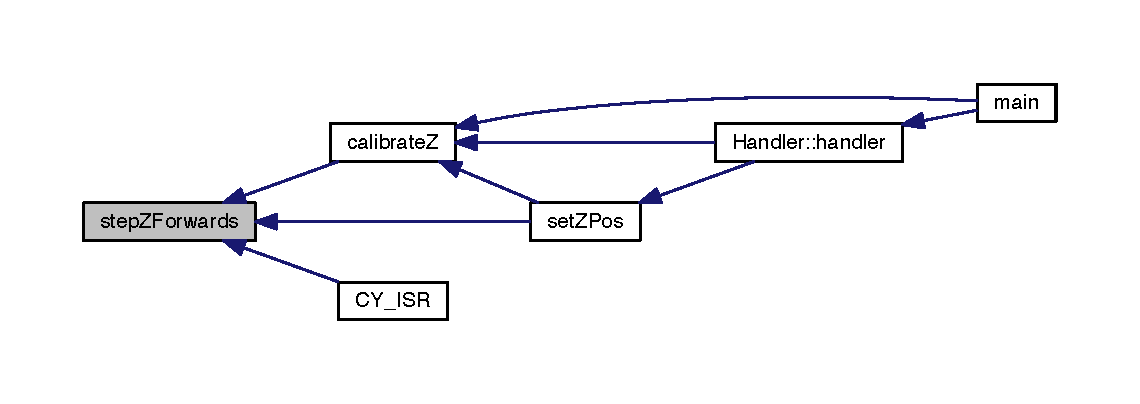
\includegraphics[width=350pt]{d7/d97/class_z_aeac8c479305ae54b347729e4ff279d44_icgraph}
\end{center}
\end{figure}


\index{Z@{Z}!z\+\_\+init@{z\+\_\+init}}
\index{z\+\_\+init@{z\+\_\+init}!Z@{Z}}
\paragraph[{\texorpdfstring{z\+\_\+init()}{z_init()}}]{\setlength{\rightskip}{0pt plus 5cm}void z\+\_\+init (
\begin{DoxyParamCaption}
\item[{void}]{}
\end{DoxyParamCaption}
)}\hypertarget{class_z_ac6bb96bf63bd2cae7c7bcc2f6b422b0c}{}\label{class_z_ac6bb96bf63bd2cae7c7bcc2f6b422b0c}


Initialiser \hyperlink{class_z}{Z} modulet. 

Initialiser \hyperlink{class_z}{Z} modulets interrupt.

\begin{DoxyAuthor}{Forfatter}
Casper Dieu Le (\href{mailto:201370338@uni.au.dk}{\tt 201370338@uni.\+au.\+dk}) 

Kasper Hinkler Uldbjerg (\href{mailto:201370281@uni.au.dk}{\tt 201370281@uni.\+au.\+dk}) 

Jeppe Stærk Antonsen (\href{mailto:201271201@uni.au.dk}{\tt 201271201@uni.\+au.\+dk}) 
\end{DoxyAuthor}


Defineret på linje 35 i filen z.\+c.



Refereret til af main().


\begin{DoxyCode}
36 \{
37   interrupt\_Z\_StartEx(isr\_Z);
38   interrupt\_S\_StartEx(isr\_S);
39 \}
\end{DoxyCode}


Her er kalder-\/grafen for denne funktion\+:
\nopagebreak
\begin{figure}[H]
\begin{center}
\leavevmode
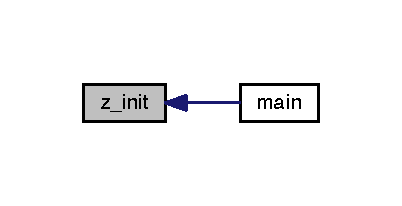
\includegraphics[width=193pt]{d7/d97/class_z_ac6bb96bf63bd2cae7c7bcc2f6b422b0c_icgraph}
\end{center}
\end{figure}


\index{Z@{Z}!z\+\_\+start@{z\+\_\+start}}
\index{z\+\_\+start@{z\+\_\+start}!Z@{Z}}
\paragraph[{\texorpdfstring{z\+\_\+start()}{z_start()}}]{\setlength{\rightskip}{0pt plus 5cm}void z\+\_\+start (
\begin{DoxyParamCaption}
\item[{void}]{}
\end{DoxyParamCaption}
)}\hypertarget{class_z_affabc649bbf2e5dbeb475777391513d7}{}\label{class_z_affabc649bbf2e5dbeb475777391513d7}


Starter \hyperlink{class_z}{Z} modulet. 

Starter \hyperlink{class_z}{Z} modulet, og køre til position 0

\begin{DoxyAuthor}{Forfatter}
Casper Dieu Le (\href{mailto:201370338@uni.au.dk}{\tt 201370338@uni.\+au.\+dk}) 

Kasper Hinkler Uldbjerg (\href{mailto:201370281@uni.au.dk}{\tt 201370281@uni.\+au.\+dk}) 

Jeppe Stærk Antonsen (\href{mailto:201271201@uni.au.dk}{\tt 201271201@uni.\+au.\+dk}) 
\end{DoxyAuthor}


Defineret på linje 50 i filen z.\+c.



Indeholder referencer til dataZ, Data\+Z\+::interruptZ, step\+Z\+Backwards() og Data\+Z\+::z\+Flag.



Refereret til af main().


\begin{DoxyCode}
51 \{
52   \hyperlink{data_8h_ace1aa5b973b9358f7236c0c9deca9370}{dataZ}.\hyperlink{data_8h_ad31cb1c3240ac1f76fc3faa902b49c24}{interruptZ} = 0;
53   DEBUG\_PutString(\textcolor{stringliteral}{"Z initializing going to zero"});
54   
55   \textcolor{keywordflow}{while}(\hyperlink{data_8h_ace1aa5b973b9358f7236c0c9deca9370}{dataZ}.\hyperlink{data_8h_ad31cb1c3240ac1f76fc3faa902b49c24}{interruptZ} == 0 && \hyperlink{data_8h_ace1aa5b973b9358f7236c0c9deca9370}{dataZ}.\hyperlink{data_8h_ac9b1acf86d4646bdf8e9f338aedb56a2}{zFlag} == 0)
56   \{
57     DEBUG\_PutString(\textcolor{stringliteral}{"."});
58     \hyperlink{class_z_ad16ddc5261a237fc03c8a4b30571c528}{stepZBackwards}();
59   \}
60   DEBUG\_PutString(\textcolor{stringliteral}{"done"});
61   DEBUG\_PutCRLF();
62   
63   \hyperlink{data_8h_ace1aa5b973b9358f7236c0c9deca9370}{dataZ}.\hyperlink{data_8h_ad31cb1c3240ac1f76fc3faa902b49c24}{interruptZ} = 0;
64 \}
\end{DoxyCode}


Her er kald-\/grafen for denne funktion\+:
\nopagebreak
\begin{figure}[H]
\begin{center}
\leavevmode
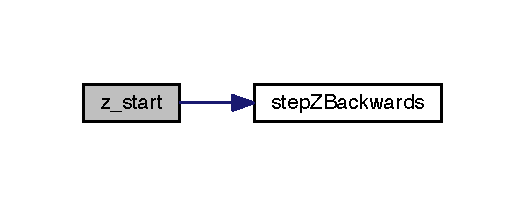
\includegraphics[width=252pt]{d7/d97/class_z_affabc649bbf2e5dbeb475777391513d7_cgraph}
\end{center}
\end{figure}




Her er kalder-\/grafen for denne funktion\+:
\nopagebreak
\begin{figure}[H]
\begin{center}
\leavevmode
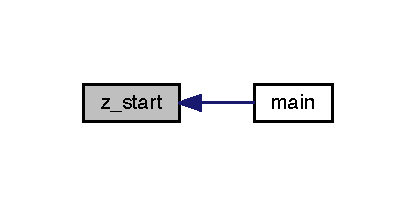
\includegraphics[width=200pt]{d7/d97/class_z_affabc649bbf2e5dbeb475777391513d7_icgraph}
\end{center}
\end{figure}




Dokumentationen for denne klasse blev genereret ud fra filerne\+:\begin{DoxyCompactItemize}
\item 
\hyperlink{z_8h}{z.\+h}\item 
\hyperlink{z_8c}{z.\+c}\end{DoxyCompactItemize}

\section{Fil-\/dokumentation}
\hypertarget{cyapicallbacks_8h}{}\subsection{cyapicallbacks.\+h filreference}
\label{cyapicallbacks_8h}\index{cyapicallbacks.\+h@{cyapicallbacks.\+h}}
Denne graf viser, hvilke filer der direkte eller indirekte inkluderer denne fil\+:
\nopagebreak
\begin{figure}[H]
\begin{center}
\leavevmode
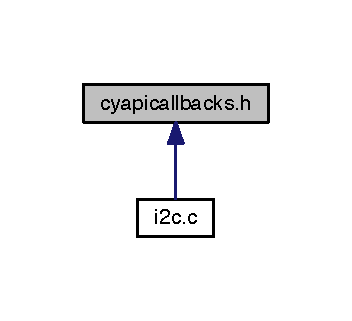
\includegraphics[width=169pt]{d4/d7d/cyapicallbacks_8h__dep__incl}
\end{center}
\end{figure}
\subsubsection*{\#Defines}
\begin{DoxyCompactItemize}
\item 
\#define \hyperlink{cyapicallbacks_8h_a696f67b7d6a9c9a1dac6387ac85b0159}{I2\+C\+S\+\_\+\+I2\+C\+\_\+\+I\+S\+R\+\_\+\+E\+X\+I\+T\+\_\+\+C\+A\+L\+L\+B\+A\+CK}
\end{DoxyCompactItemize}
\subsubsection*{Funktioner}
\begin{DoxyCompactItemize}
\item 
void \hyperlink{cyapicallbacks_8h_ab1cc1a553a438e7390297df1a2181173}{I2\+C\+S\+\_\+\+I2\+C\+\_\+\+I\+S\+R\+\_\+\+Exit\+Callback} (void)
\end{DoxyCompactItemize}


\subsubsection{\#Define-\/dokumentation}
\index{cyapicallbacks.\+h@{cyapicallbacks.\+h}!I2\+C\+S\+\_\+\+I2\+C\+\_\+\+I\+S\+R\+\_\+\+E\+X\+I\+T\+\_\+\+C\+A\+L\+L\+B\+A\+CK@{I2\+C\+S\+\_\+\+I2\+C\+\_\+\+I\+S\+R\+\_\+\+E\+X\+I\+T\+\_\+\+C\+A\+L\+L\+B\+A\+CK}}
\index{I2\+C\+S\+\_\+\+I2\+C\+\_\+\+I\+S\+R\+\_\+\+E\+X\+I\+T\+\_\+\+C\+A\+L\+L\+B\+A\+CK@{I2\+C\+S\+\_\+\+I2\+C\+\_\+\+I\+S\+R\+\_\+\+E\+X\+I\+T\+\_\+\+C\+A\+L\+L\+B\+A\+CK}!cyapicallbacks.\+h@{cyapicallbacks.\+h}}
\paragraph[{\texorpdfstring{I2\+C\+S\+\_\+\+I2\+C\+\_\+\+I\+S\+R\+\_\+\+E\+X\+I\+T\+\_\+\+C\+A\+L\+L\+B\+A\+CK}{I2CS_I2C_ISR_EXIT_CALLBACK}}]{\setlength{\rightskip}{0pt plus 5cm}\#define I2\+C\+S\+\_\+\+I2\+C\+\_\+\+I\+S\+R\+\_\+\+E\+X\+I\+T\+\_\+\+C\+A\+L\+L\+B\+A\+CK}\hypertarget{cyapicallbacks_8h_a696f67b7d6a9c9a1dac6387ac85b0159}{}\label{cyapicallbacks_8h_a696f67b7d6a9c9a1dac6387ac85b0159}


Defineret på linje 15 i filen cyapicallbacks.\+h.



\subsubsection{Funktions-\/dokumentation}
\index{cyapicallbacks.\+h@{cyapicallbacks.\+h}!I2\+C\+S\+\_\+\+I2\+C\+\_\+\+I\+S\+R\+\_\+\+Exit\+Callback@{I2\+C\+S\+\_\+\+I2\+C\+\_\+\+I\+S\+R\+\_\+\+Exit\+Callback}}
\index{I2\+C\+S\+\_\+\+I2\+C\+\_\+\+I\+S\+R\+\_\+\+Exit\+Callback@{I2\+C\+S\+\_\+\+I2\+C\+\_\+\+I\+S\+R\+\_\+\+Exit\+Callback}!cyapicallbacks.\+h@{cyapicallbacks.\+h}}
\paragraph[{\texorpdfstring{I2\+C\+S\+\_\+\+I2\+C\+\_\+\+I\+S\+R\+\_\+\+Exit\+Callback(void)}{I2CS_I2C_ISR_ExitCallback(void)}}]{\setlength{\rightskip}{0pt plus 5cm}void I2\+C\+S\+\_\+\+I2\+C\+\_\+\+I\+S\+R\+\_\+\+Exit\+Callback (
\begin{DoxyParamCaption}
\item[{void}]{}
\end{DoxyParamCaption}
)}\hypertarget{cyapicallbacks_8h_ab1cc1a553a438e7390297df1a2181173}{}\label{cyapicallbacks_8h_ab1cc1a553a438e7390297df1a2181173}

\hypertarget{data_8c}{}\subsection{data.\+c filreference}
\label{data_8c}\index{data.\+c@{data.\+c}}


\hyperlink{class_data}{Data} modul.  


{\ttfamily \#include \char`\"{}data.\+h\char`\"{}}\\*
Inklusions-\/afhængighedsgraf for data.\+c\+:
\nopagebreak
\begin{figure}[H]
\begin{center}
\leavevmode
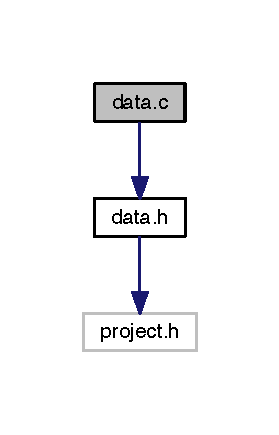
\includegraphics[width=134pt]{de/dce/data_8c__incl}
\end{center}
\end{figure}


\subsubsection{Detaljeret beskrivelse}
\hyperlink{class_data}{Data} modul. 

Indeholder data vedr. \hyperlink{class_z}{Z} modulet. \begin{DoxyAuthor}{Forfatter}
Jeppe Stærk Antonsen (\href{mailto:201271201@uni.au.dk}{\tt 201271201@uni.\+au.\+dk}) 
\end{DoxyAuthor}

\hypertarget{data_8h}{}\subsection{data.\+h filreference}
\label{data_8h}\index{data.\+h@{data.\+h}}


\hyperlink{class_data}{Data} modul.  


{\ttfamily \#include $<$project.\+h$>$}\\*
Inklusions-\/afhængighedsgraf for data.\+h\+:
\nopagebreak
\begin{figure}[H]
\begin{center}
\leavevmode
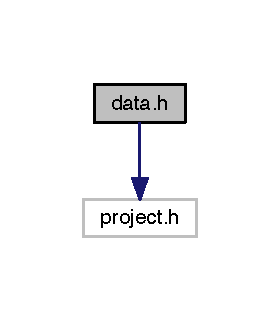
\includegraphics[width=134pt]{d6/d2b/data_8h__incl}
\end{center}
\end{figure}
Denne graf viser, hvilke filer der direkte eller indirekte inkluderer denne fil\+:
\nopagebreak
\begin{figure}[H]
\begin{center}
\leavevmode
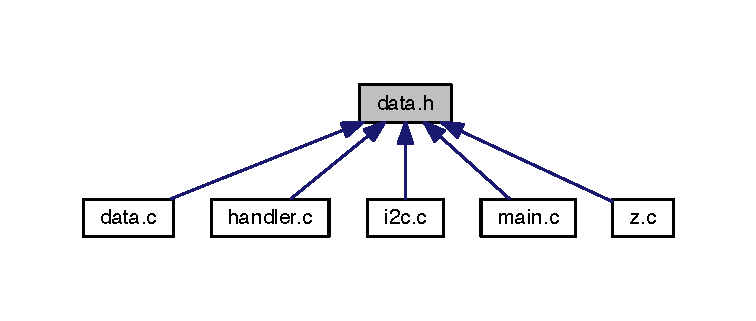
\includegraphics[width=350pt]{d2/d2f/data_8h__dep__incl}
\end{center}
\end{figure}
\subsubsection*{Datastrukturer}
\begin{DoxyCompactItemize}
\item 
struct \hyperlink{data_8h_df/d4b/struct_data_x_y}{Data\+XY}
\end{DoxyCompactItemize}
\subsubsection*{Funktioner}
\begin{DoxyCompactItemize}
\item 
void \hyperlink{data_8h_adf37c815716edf228a3cbb4564290275}{data\+\_\+init} (void)
\end{DoxyCompactItemize}
\subsubsection*{Variable}
\begin{DoxyCompactItemize}
\item 
struct \hyperlink{data_8h_df/d4b/struct_data_x_y}{Data\+XY} \hyperlink{data_8h_a89d7998a721b3f36f9f4131e7a5e42d2}{data\+XY}
\end{DoxyCompactItemize}


\subsubsection{Detaljeret beskrivelse}
\hyperlink{class_data}{Data} modul. 

Indeholder data vedr. \hyperlink{class_x_y}{XY} modulet. \begin{DoxyAuthor}{Forfatter}
Casper Dieu Le (\href{mailto:201370338@uni.au.dk}{\tt 201370338@uni.\+au.\+dk}) 

Kasper Hinkler Uldbjerg (\href{mailto:201370281@uni.au.dk}{\tt 201370281@uni.\+au.\+dk}) 

Jeppe Stærk Antonsen (\href{mailto:201271201@uni.au.dk}{\tt 201271201@uni.\+au.\+dk}) 
\end{DoxyAuthor}


\subsubsection{Datastruktur-\/documentation}
\index{Data\+XY@{Data\+XY}}\label{struct_data_x_y}
\hypertarget{data_8h_struct_data_x_y}{}
\paragraph{struct Data\+XY}


Defineret på linje 32 i filen data.\+h.



Samarbejdsdiagram for Data\+XY\+:
\nopagebreak
\begin{figure}[H]
\begin{center}
\leavevmode
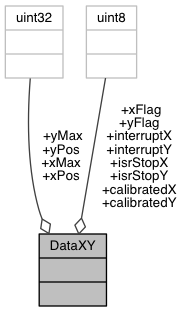
\includegraphics[width=208pt]{de/d6c/struct_data_x_y__coll__graph}
\end{center}
\end{figure}
\begin{DoxyFields}{Data-\/felter}
uint8\hypertarget{data_8h_a20403c23f502143a2dd7ee5bb641c0ab}{}\label{data_8h_a20403c23f502143a2dd7ee5bb641c0ab}
&
calibratedX&
\\
\hline

uint8\hypertarget{data_8h_adebeaa27d72b604babe006a478cfed16}{}\label{data_8h_adebeaa27d72b604babe006a478cfed16}
&
calibratedY&
\\
\hline

uint8\hypertarget{data_8h_a4cacb2964bb4b589bf79aa64a398725b}{}\label{data_8h_a4cacb2964bb4b589bf79aa64a398725b}
&
interruptX&
\\
\hline

uint8\hypertarget{data_8h_a0149ea97a32442280eb1c0b30c1eeaf1}{}\label{data_8h_a0149ea97a32442280eb1c0b30c1eeaf1}
&
interruptY&
\\
\hline

uint8\hypertarget{data_8h_ab8211b7be27d53644048a83fccb95d70}{}\label{data_8h_ab8211b7be27d53644048a83fccb95d70}
&
isr\+StopX&
\\
\hline

uint8\hypertarget{data_8h_a92ec85e6a09f5dc7ed83640f1810c4bb}{}\label{data_8h_a92ec85e6a09f5dc7ed83640f1810c4bb}
&
isr\+StopY&
\\
\hline

uint8\hypertarget{data_8h_abd60bb18cb69d4a782e0334caad9ffbc}{}\label{data_8h_abd60bb18cb69d4a782e0334caad9ffbc}
&
x\+Flag&
\\
\hline

uint32\hypertarget{data_8h_a5b6ae90a32a5f290afcc50656befceca}{}\label{data_8h_a5b6ae90a32a5f290afcc50656befceca}
&
x\+Max&
\\
\hline

uint32\hypertarget{data_8h_a5262e09f478a571552e65be75c506bdb}{}\label{data_8h_a5262e09f478a571552e65be75c506bdb}
&
x\+Pos&
\\
\hline

uint8\hypertarget{data_8h_a2093b99c34cd9ec2a282b9c4c3f61935}{}\label{data_8h_a2093b99c34cd9ec2a282b9c4c3f61935}
&
y\+Flag&
\\
\hline

uint32\hypertarget{data_8h_ab979b62fb4882313ad47718325e34879}{}\label{data_8h_ab979b62fb4882313ad47718325e34879}
&
y\+Max&
\\
\hline

uint32\hypertarget{data_8h_a4c7347df04ab0f3d860046571be08af4}{}\label{data_8h_a4c7347df04ab0f3d860046571be08af4}
&
y\+Pos&
\\
\hline

\end{DoxyFields}


\subsubsection{Funktions-\/dokumentation}
\index{data.\+h@{data.\+h}!data\+\_\+init@{data\+\_\+init}}
\index{data\+\_\+init@{data\+\_\+init}!data.\+h@{data.\+h}}
\paragraph[{\texorpdfstring{data\+\_\+init(void)}{data_init(void)}}]{\setlength{\rightskip}{0pt plus 5cm}void data\+\_\+init (
\begin{DoxyParamCaption}
\item[{void}]{}
\end{DoxyParamCaption}
)}\hypertarget{data_8h_adf37c815716edf228a3cbb4564290275}{}\label{data_8h_adf37c815716edf228a3cbb4564290275}


\subsubsection{Variabel-\/dokumentation}
\index{data.\+h@{data.\+h}!data\+XY@{data\+XY}}
\index{data\+XY@{data\+XY}!data.\+h@{data.\+h}}
\paragraph[{\texorpdfstring{data\+XY}{dataXY}}]{\setlength{\rightskip}{0pt plus 5cm}struct {\bf Data\+XY} data\+XY}\hypertarget{data_8h_a89d7998a721b3f36f9f4131e7a5e42d2}{}\label{data_8h_a89d7998a721b3f36f9f4131e7a5e42d2}


Refereret til af X\+Y\+::calibrate\+X(), X\+Y\+::calibrate\+Y(), X\+Y\+::\+C\+Y\+\_\+\+I\+S\+R(), Data\+::data\+\_\+init(), Handler\+::handler(), I2\+C\+::\+I2\+C\+S\+\_\+\+I2\+C\+\_\+\+I\+S\+R\+\_\+\+Exit\+Callback(), X\+Y\+::set\+X\+Pos(), X\+Y\+::set\+Y\+Pos() og X\+Y\+::xy\+\_\+start().


\hypertarget{handler_8c}{}\subsection{handler.\+c filreference}
\label{handler_8c}\index{handler.\+c@{handler.\+c}}


\hyperlink{class_handler}{Handler} modul.  


{\ttfamily \#include \char`\"{}handler.\+h\char`\"{}}\\*
{\ttfamily \#include \char`\"{}data.\+h\char`\"{}}\\*
{\ttfamily \#include \char`\"{}i2c.\+h\char`\"{}}\\*
{\ttfamily \#include \char`\"{}spi.\+h\char`\"{}}\\*
{\ttfamily \#include $<$stdio.\+h$>$}\\*
Inklusions-\/afhængighedsgraf for handler.\+c\+:\nopagebreak
\begin{figure}[H]
\begin{center}
\leavevmode
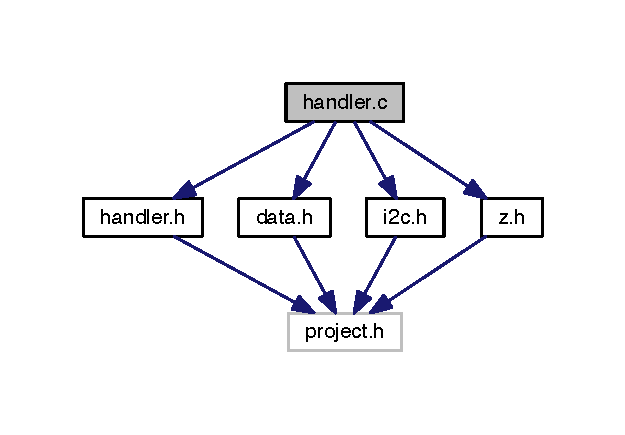
\includegraphics[width=350pt]{d2/d83/handler_8c__incl}
\end{center}
\end{figure}


\subsubsection{Detaljeret beskrivelse}
\hyperlink{class_handler}{Handler} modul. 

Håndtere indkommende kommandoer med tilhørende værdier. \begin{DoxyAuthor}{Forfatter}
Jeppe Stærk Antonsen (\href{mailto:201271201@uni.au.dk}{\tt 201271201@uni.\+au.\+dk}) 
\end{DoxyAuthor}

\hypertarget{handler_8h}{}\subsection{handler.\+h filreference}
\label{handler_8h}\index{handler.\+h@{handler.\+h}}


\hyperlink{class_handler}{Handler} modul.  


{\ttfamily \#include $<$project.\+h$>$}\\*
Inklusions-\/afhængighedsgraf for handler.\+h\+:
\nopagebreak
\begin{figure}[H]
\begin{center}
\leavevmode
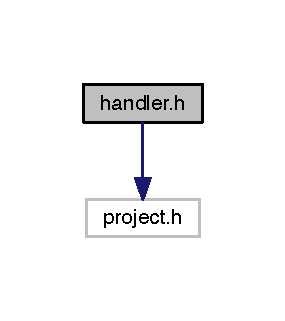
\includegraphics[width=137pt]{db/d41/handler_8h__incl}
\end{center}
\end{figure}
Denne graf viser, hvilke filer der direkte eller indirekte inkluderer denne fil\+:
\nopagebreak
\begin{figure}[H]
\begin{center}
\leavevmode
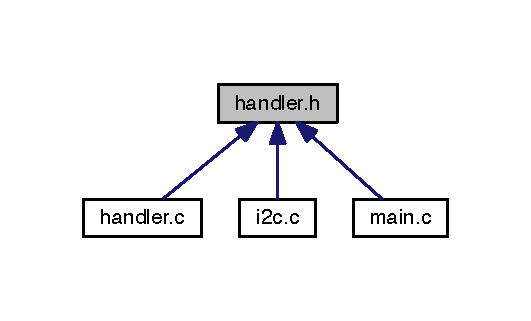
\includegraphics[width=255pt]{d4/d76/handler_8h__dep__incl}
\end{center}
\end{figure}
\subsubsection*{\#Defines}
\begin{DoxyCompactItemize}
\item 
\#define \hyperlink{handler_8h_af70b73890a98cfe329a916df037f46a4}{C\+M\+D\+\_\+\+S\+E\+T\+\_\+\+X\+\_\+\+P\+OS}~(0x10u)
\item 
\#define \hyperlink{handler_8h_a82640a671f668fb40ff4851901d5a151}{C\+M\+D\+\_\+\+S\+E\+T\+\_\+\+Y\+\_\+\+P\+OS}~(0x11u)
\item 
\#define \hyperlink{handler_8h_aa50e083669624eeaef782ebc867008f9}{C\+M\+D\+\_\+\+G\+E\+T\+\_\+\+X\+\_\+\+P\+OS}~(0x12u)
\item 
\#define \hyperlink{handler_8h_a51053e5251048d6ebbf4d2e23de40761}{C\+M\+D\+\_\+\+G\+E\+T\+\_\+\+Y\+\_\+\+P\+OS}~(0x13u)
\item 
\#define \hyperlink{handler_8h_ad9bda4ca0abdec2ab1e6506761623671}{C\+M\+D\+\_\+\+G\+E\+T\+\_\+\+X\+\_\+\+M\+AX}~(0x14u)
\item 
\#define \hyperlink{handler_8h_ab73a35345dedba2dcb9641488e8ddadd}{C\+M\+D\+\_\+\+G\+E\+T\+\_\+\+Y\+\_\+\+M\+AX}~(0x15u)
\item 
\#define \hyperlink{handler_8h_af7c8f19d1c1b9e2240251d42109c5cfd}{C\+M\+D\+\_\+\+X\+\_\+\+S\+TP}~(0x16u)
\item 
\#define \hyperlink{handler_8h_a83ab3037b2c91ea010b2d8c47acd5434}{C\+M\+D\+\_\+\+Y\+\_\+\+S\+TP}~(0x17u)
\item 
\#define \hyperlink{handler_8h_a5edf35288955238e1090f2367f96e828}{C\+M\+D\+\_\+\+X\+\_\+\+C\+AL}~(0x18u)
\item 
\#define \hyperlink{handler_8h_a2b2db51eef91dc2aa5586d0817838ef2}{C\+M\+D\+\_\+\+Y\+\_\+\+C\+AL}~(0x19u)
\item 
\#define \hyperlink{handler_8h_a6e695093ea021ccac7cc5d2d788095c9}{C\+M\+D\+\_\+\+S\+E\+T\+\_\+\+Z\+\_\+\+P\+OS}~(0x20u)
\item 
\#define \hyperlink{handler_8h_a4d76e78d09a00f75609569d9aa92ab98}{C\+M\+D\+\_\+\+G\+E\+T\+\_\+\+Z\+\_\+\+P\+OS}~(0x21u)
\item 
\#define \hyperlink{handler_8h_a188e7cab5d0cf0e363a20c5abcdab482}{C\+M\+D\+\_\+\+G\+E\+T\+\_\+\+Z\+\_\+\+M\+AX}~(0x22u)
\item 
\#define \hyperlink{handler_8h_ad119aef78e8cb8e9aa12f35aeae94a99}{C\+M\+D\+\_\+\+Z\+\_\+\+S\+TP}~(0x23u)
\item 
\#define \hyperlink{handler_8h_ab77bdaae57e9e34f7bfc1d1a31213f94}{C\+M\+D\+\_\+\+Z\+\_\+\+C\+AL}~(0x24u)
\item 
\#define \hyperlink{handler_8h_afc24de4a99d70315d939185a1c3d61f0}{C\+M\+D\+\_\+\+S\+E\+T\+\_\+\+R\+E\+D\+\_\+\+V\+AL}~(0x30u)
\item 
\#define \hyperlink{handler_8h_a24acd29fea2e546409449638b79ac094}{C\+M\+D\+\_\+\+S\+E\+T\+\_\+\+G\+R\+E\+E\+N\+\_\+\+V\+AL}~(0x31u)
\item 
\#define \hyperlink{handler_8h_a4ab3ea64ee56aef3a566698b8959df51}{C\+M\+D\+\_\+\+S\+E\+T\+\_\+\+B\+L\+U\+E\+\_\+\+V\+AL}~(0x32u)
\item 
\#define \hyperlink{handler_8h_a3f217d17f4b67e6b46eb294ab3db2e87}{C\+M\+D\+\_\+\+S\+E\+T\+\_\+\+L\+U\+M\+E\+N\+\_\+\+V\+AL}~(0x33u)
\item 
\#define \hyperlink{handler_8h_a1fe6f15c7c98032dc2bd2a1417977fcf}{C\+M\+D\+\_\+\+S\+E\+T\+\_\+\+P\+O\+W\+E\+R\+\_\+\+S\+TS}~(0x34u)
\item 
\#define \hyperlink{handler_8h_aa2f09e60c4eeae4560da88c6b1b08c60}{C\+M\+D\+\_\+\+G\+E\+T\+\_\+\+R\+E\+D\+\_\+\+V\+AL}~(0x35u)
\item 
\#define \hyperlink{handler_8h_a55d24f50aeb52afddd491d97a66c81ef}{C\+M\+D\+\_\+\+G\+E\+T\+\_\+\+G\+R\+E\+E\+N\+\_\+\+V\+AL}~(0x36u)
\item 
\#define \hyperlink{handler_8h_a81052c67f996705d7eacfcea66bdde08}{C\+M\+D\+\_\+\+G\+E\+T\+\_\+\+B\+L\+U\+E\+\_\+\+V\+AL}~(0x37u)
\item 
\#define \hyperlink{handler_8h_a8ed7ad21a658c878390e9cec4d45aab5}{C\+M\+D\+\_\+\+G\+E\+T\+\_\+\+L\+U\+M\+E\+N\+\_\+\+V\+AL}~(0x38u)
\item 
\#define \hyperlink{handler_8h_ab9e8683e41e93fd467b170c321a1c685}{C\+M\+D\+\_\+\+G\+E\+T\+\_\+\+P\+O\+W\+E\+R\+\_\+\+S\+TS}~(0x39u)
\item 
\#define \hyperlink{handler_8h_a67cc7e7270e79a6e95be2e25cac29feb}{C\+M\+D\+\_\+\+S\+E\+T\+\_\+\+D\+I\+S\+T\+A\+N\+C\+E\+\_\+\+S\+TS}~(0x40u)
\item 
\#define \hyperlink{handler_8h_a84f8a23b131cb2b163e16889afd9ef85}{C\+M\+D\+\_\+\+S\+E\+T\+\_\+\+M\+O\+V\+E\+M\+E\+N\+T\+\_\+\+S\+TS}~(0x41u)
\item 
\#define \hyperlink{handler_8h_a8ea17eed84662f9389bfa1751c03a4b2}{C\+M\+D\+\_\+\+G\+E\+T\+\_\+\+D\+I\+S\+T\+A\+N\+C\+E\+\_\+\+S\+TS}~(0x42u)
\item 
\#define \hyperlink{handler_8h_a4adcfb68de1b319e19342143cb61b550}{C\+M\+D\+\_\+\+G\+E\+T\+\_\+\+M\+O\+V\+E\+M\+E\+N\+T\+\_\+\+S\+TS}~(0x43u)
\item 
\#define \hyperlink{handler_8h_a17dc606d3dbd6f9d4ca831cb02c91af0}{C\+M\+D\+\_\+\+D\+I\+S\+T\+A\+N\+C\+E\+\_\+\+A\+L\+RT}~(0x44u)
\item 
\#define \hyperlink{handler_8h_a7bd43223cfa796f0289d0548e090bbcc}{C\+M\+D\+\_\+\+M\+O\+V\+E\+M\+E\+N\+T\+\_\+\+A\+L\+RT}~(0x45u)
\end{DoxyCompactItemize}
\subsubsection*{Funktioner}
\begin{DoxyCompactItemize}
\item 
void \hyperlink{handler_8h_af5be5b016b862943cd22504490acc8f4}{handler} (uint8 cmd, uint8 val)
\end{DoxyCompactItemize}


\subsubsection{Detaljeret beskrivelse}
\hyperlink{class_handler}{Handler} modul. 

Håndtere indkommende kommandoer med tilhørende værdier. \begin{DoxyAuthor}{Forfatter}
Jeppe Stærk Antonsen (\href{mailto:201271201@uni.au.dk}{\tt 201271201@uni.\+au.\+dk}) 
\end{DoxyAuthor}


\subsubsection{\#Define-\/dokumentation}
\index{handler.\+h@{handler.\+h}!C\+M\+D\+\_\+\+D\+I\+S\+T\+A\+N\+C\+E\+\_\+\+A\+L\+RT@{C\+M\+D\+\_\+\+D\+I\+S\+T\+A\+N\+C\+E\+\_\+\+A\+L\+RT}}
\index{C\+M\+D\+\_\+\+D\+I\+S\+T\+A\+N\+C\+E\+\_\+\+A\+L\+RT@{C\+M\+D\+\_\+\+D\+I\+S\+T\+A\+N\+C\+E\+\_\+\+A\+L\+RT}!handler.\+h@{handler.\+h}}
\paragraph[{\texorpdfstring{C\+M\+D\+\_\+\+D\+I\+S\+T\+A\+N\+C\+E\+\_\+\+A\+L\+RT}{CMD_DISTANCE_ALRT}}]{\setlength{\rightskip}{0pt plus 5cm}\#define C\+M\+D\+\_\+\+D\+I\+S\+T\+A\+N\+C\+E\+\_\+\+A\+L\+RT~(0x44u)}\hypertarget{handler_8h_a17dc606d3dbd6f9d4ca831cb02c91af0}{}\label{handler_8h_a17dc606d3dbd6f9d4ca831cb02c91af0}


Defineret på linje 65 i filen handler.\+h.



Refereret til af Handler\+::handler().

\index{handler.\+h@{handler.\+h}!C\+M\+D\+\_\+\+G\+E\+T\+\_\+\+B\+L\+U\+E\+\_\+\+V\+AL@{C\+M\+D\+\_\+\+G\+E\+T\+\_\+\+B\+L\+U\+E\+\_\+\+V\+AL}}
\index{C\+M\+D\+\_\+\+G\+E\+T\+\_\+\+B\+L\+U\+E\+\_\+\+V\+AL@{C\+M\+D\+\_\+\+G\+E\+T\+\_\+\+B\+L\+U\+E\+\_\+\+V\+AL}!handler.\+h@{handler.\+h}}
\paragraph[{\texorpdfstring{C\+M\+D\+\_\+\+G\+E\+T\+\_\+\+B\+L\+U\+E\+\_\+\+V\+AL}{CMD_GET_BLUE_VAL}}]{\setlength{\rightskip}{0pt plus 5cm}\#define C\+M\+D\+\_\+\+G\+E\+T\+\_\+\+B\+L\+U\+E\+\_\+\+V\+AL~(0x37u)}\hypertarget{handler_8h_a81052c67f996705d7eacfcea66bdde08}{}\label{handler_8h_a81052c67f996705d7eacfcea66bdde08}


Defineret på linje 58 i filen handler.\+h.



Refereret til af S\+P\+I\+::\+C\+Y\+\_\+\+I\+S\+R() og Handler\+::handler().

\index{handler.\+h@{handler.\+h}!C\+M\+D\+\_\+\+G\+E\+T\+\_\+\+D\+I\+S\+T\+A\+N\+C\+E\+\_\+\+S\+TS@{C\+M\+D\+\_\+\+G\+E\+T\+\_\+\+D\+I\+S\+T\+A\+N\+C\+E\+\_\+\+S\+TS}}
\index{C\+M\+D\+\_\+\+G\+E\+T\+\_\+\+D\+I\+S\+T\+A\+N\+C\+E\+\_\+\+S\+TS@{C\+M\+D\+\_\+\+G\+E\+T\+\_\+\+D\+I\+S\+T\+A\+N\+C\+E\+\_\+\+S\+TS}!handler.\+h@{handler.\+h}}
\paragraph[{\texorpdfstring{C\+M\+D\+\_\+\+G\+E\+T\+\_\+\+D\+I\+S\+T\+A\+N\+C\+E\+\_\+\+S\+TS}{CMD_GET_DISTANCE_STS}}]{\setlength{\rightskip}{0pt plus 5cm}\#define C\+M\+D\+\_\+\+G\+E\+T\+\_\+\+D\+I\+S\+T\+A\+N\+C\+E\+\_\+\+S\+TS~(0x42u)}\hypertarget{handler_8h_a8ea17eed84662f9389bfa1751c03a4b2}{}\label{handler_8h_a8ea17eed84662f9389bfa1751c03a4b2}


Defineret på linje 63 i filen handler.\+h.



Refereret til af Handler\+::handler().

\index{handler.\+h@{handler.\+h}!C\+M\+D\+\_\+\+G\+E\+T\+\_\+\+G\+R\+E\+E\+N\+\_\+\+V\+AL@{C\+M\+D\+\_\+\+G\+E\+T\+\_\+\+G\+R\+E\+E\+N\+\_\+\+V\+AL}}
\index{C\+M\+D\+\_\+\+G\+E\+T\+\_\+\+G\+R\+E\+E\+N\+\_\+\+V\+AL@{C\+M\+D\+\_\+\+G\+E\+T\+\_\+\+G\+R\+E\+E\+N\+\_\+\+V\+AL}!handler.\+h@{handler.\+h}}
\paragraph[{\texorpdfstring{C\+M\+D\+\_\+\+G\+E\+T\+\_\+\+G\+R\+E\+E\+N\+\_\+\+V\+AL}{CMD_GET_GREEN_VAL}}]{\setlength{\rightskip}{0pt plus 5cm}\#define C\+M\+D\+\_\+\+G\+E\+T\+\_\+\+G\+R\+E\+E\+N\+\_\+\+V\+AL~(0x36u)}\hypertarget{handler_8h_a55d24f50aeb52afddd491d97a66c81ef}{}\label{handler_8h_a55d24f50aeb52afddd491d97a66c81ef}


Defineret på linje 57 i filen handler.\+h.



Refereret til af S\+P\+I\+::\+C\+Y\+\_\+\+I\+S\+R() og Handler\+::handler().

\index{handler.\+h@{handler.\+h}!C\+M\+D\+\_\+\+G\+E\+T\+\_\+\+L\+U\+M\+E\+N\+\_\+\+V\+AL@{C\+M\+D\+\_\+\+G\+E\+T\+\_\+\+L\+U\+M\+E\+N\+\_\+\+V\+AL}}
\index{C\+M\+D\+\_\+\+G\+E\+T\+\_\+\+L\+U\+M\+E\+N\+\_\+\+V\+AL@{C\+M\+D\+\_\+\+G\+E\+T\+\_\+\+L\+U\+M\+E\+N\+\_\+\+V\+AL}!handler.\+h@{handler.\+h}}
\paragraph[{\texorpdfstring{C\+M\+D\+\_\+\+G\+E\+T\+\_\+\+L\+U\+M\+E\+N\+\_\+\+V\+AL}{CMD_GET_LUMEN_VAL}}]{\setlength{\rightskip}{0pt plus 5cm}\#define C\+M\+D\+\_\+\+G\+E\+T\+\_\+\+L\+U\+M\+E\+N\+\_\+\+V\+AL~(0x38u)}\hypertarget{handler_8h_a8ed7ad21a658c878390e9cec4d45aab5}{}\label{handler_8h_a8ed7ad21a658c878390e9cec4d45aab5}


Defineret på linje 59 i filen handler.\+h.



Refereret til af Handler\+::handler().

\index{handler.\+h@{handler.\+h}!C\+M\+D\+\_\+\+G\+E\+T\+\_\+\+M\+O\+V\+E\+M\+E\+N\+T\+\_\+\+S\+TS@{C\+M\+D\+\_\+\+G\+E\+T\+\_\+\+M\+O\+V\+E\+M\+E\+N\+T\+\_\+\+S\+TS}}
\index{C\+M\+D\+\_\+\+G\+E\+T\+\_\+\+M\+O\+V\+E\+M\+E\+N\+T\+\_\+\+S\+TS@{C\+M\+D\+\_\+\+G\+E\+T\+\_\+\+M\+O\+V\+E\+M\+E\+N\+T\+\_\+\+S\+TS}!handler.\+h@{handler.\+h}}
\paragraph[{\texorpdfstring{C\+M\+D\+\_\+\+G\+E\+T\+\_\+\+M\+O\+V\+E\+M\+E\+N\+T\+\_\+\+S\+TS}{CMD_GET_MOVEMENT_STS}}]{\setlength{\rightskip}{0pt plus 5cm}\#define C\+M\+D\+\_\+\+G\+E\+T\+\_\+\+M\+O\+V\+E\+M\+E\+N\+T\+\_\+\+S\+TS~(0x43u)}\hypertarget{handler_8h_a4adcfb68de1b319e19342143cb61b550}{}\label{handler_8h_a4adcfb68de1b319e19342143cb61b550}


Defineret på linje 64 i filen handler.\+h.



Refereret til af Handler\+::handler().

\index{handler.\+h@{handler.\+h}!C\+M\+D\+\_\+\+G\+E\+T\+\_\+\+P\+O\+W\+E\+R\+\_\+\+S\+TS@{C\+M\+D\+\_\+\+G\+E\+T\+\_\+\+P\+O\+W\+E\+R\+\_\+\+S\+TS}}
\index{C\+M\+D\+\_\+\+G\+E\+T\+\_\+\+P\+O\+W\+E\+R\+\_\+\+S\+TS@{C\+M\+D\+\_\+\+G\+E\+T\+\_\+\+P\+O\+W\+E\+R\+\_\+\+S\+TS}!handler.\+h@{handler.\+h}}
\paragraph[{\texorpdfstring{C\+M\+D\+\_\+\+G\+E\+T\+\_\+\+P\+O\+W\+E\+R\+\_\+\+S\+TS}{CMD_GET_POWER_STS}}]{\setlength{\rightskip}{0pt plus 5cm}\#define C\+M\+D\+\_\+\+G\+E\+T\+\_\+\+P\+O\+W\+E\+R\+\_\+\+S\+TS~(0x39u)}\hypertarget{handler_8h_ab9e8683e41e93fd467b170c321a1c685}{}\label{handler_8h_ab9e8683e41e93fd467b170c321a1c685}


Defineret på linje 60 i filen handler.\+h.



Refereret til af Handler\+::handler().

\index{handler.\+h@{handler.\+h}!C\+M\+D\+\_\+\+G\+E\+T\+\_\+\+R\+E\+D\+\_\+\+V\+AL@{C\+M\+D\+\_\+\+G\+E\+T\+\_\+\+R\+E\+D\+\_\+\+V\+AL}}
\index{C\+M\+D\+\_\+\+G\+E\+T\+\_\+\+R\+E\+D\+\_\+\+V\+AL@{C\+M\+D\+\_\+\+G\+E\+T\+\_\+\+R\+E\+D\+\_\+\+V\+AL}!handler.\+h@{handler.\+h}}
\paragraph[{\texorpdfstring{C\+M\+D\+\_\+\+G\+E\+T\+\_\+\+R\+E\+D\+\_\+\+V\+AL}{CMD_GET_RED_VAL}}]{\setlength{\rightskip}{0pt plus 5cm}\#define C\+M\+D\+\_\+\+G\+E\+T\+\_\+\+R\+E\+D\+\_\+\+V\+AL~(0x35u)}\hypertarget{handler_8h_aa2f09e60c4eeae4560da88c6b1b08c60}{}\label{handler_8h_aa2f09e60c4eeae4560da88c6b1b08c60}


Defineret på linje 56 i filen handler.\+h.



Refereret til af S\+P\+I\+::\+C\+Y\+\_\+\+I\+S\+R() og Handler\+::handler().

\index{handler.\+h@{handler.\+h}!C\+M\+D\+\_\+\+G\+E\+T\+\_\+\+X\+\_\+\+M\+AX@{C\+M\+D\+\_\+\+G\+E\+T\+\_\+\+X\+\_\+\+M\+AX}}
\index{C\+M\+D\+\_\+\+G\+E\+T\+\_\+\+X\+\_\+\+M\+AX@{C\+M\+D\+\_\+\+G\+E\+T\+\_\+\+X\+\_\+\+M\+AX}!handler.\+h@{handler.\+h}}
\paragraph[{\texorpdfstring{C\+M\+D\+\_\+\+G\+E\+T\+\_\+\+X\+\_\+\+M\+AX}{CMD_GET_X_MAX}}]{\setlength{\rightskip}{0pt plus 5cm}\#define C\+M\+D\+\_\+\+G\+E\+T\+\_\+\+X\+\_\+\+M\+AX~(0x14u)}\hypertarget{handler_8h_ad9bda4ca0abdec2ab1e6506761623671}{}\label{handler_8h_ad9bda4ca0abdec2ab1e6506761623671}


Defineret på linje 40 i filen handler.\+h.

\index{handler.\+h@{handler.\+h}!C\+M\+D\+\_\+\+G\+E\+T\+\_\+\+X\+\_\+\+P\+OS@{C\+M\+D\+\_\+\+G\+E\+T\+\_\+\+X\+\_\+\+P\+OS}}
\index{C\+M\+D\+\_\+\+G\+E\+T\+\_\+\+X\+\_\+\+P\+OS@{C\+M\+D\+\_\+\+G\+E\+T\+\_\+\+X\+\_\+\+P\+OS}!handler.\+h@{handler.\+h}}
\paragraph[{\texorpdfstring{C\+M\+D\+\_\+\+G\+E\+T\+\_\+\+X\+\_\+\+P\+OS}{CMD_GET_X_POS}}]{\setlength{\rightskip}{0pt plus 5cm}\#define C\+M\+D\+\_\+\+G\+E\+T\+\_\+\+X\+\_\+\+P\+OS~(0x12u)}\hypertarget{handler_8h_aa50e083669624eeaef782ebc867008f9}{}\label{handler_8h_aa50e083669624eeaef782ebc867008f9}


Defineret på linje 38 i filen handler.\+h.



Refereret til af S\+P\+I\+::\+C\+Y\+\_\+\+I\+S\+R() og Handler\+::handler().

\index{handler.\+h@{handler.\+h}!C\+M\+D\+\_\+\+G\+E\+T\+\_\+\+Y\+\_\+\+M\+AX@{C\+M\+D\+\_\+\+G\+E\+T\+\_\+\+Y\+\_\+\+M\+AX}}
\index{C\+M\+D\+\_\+\+G\+E\+T\+\_\+\+Y\+\_\+\+M\+AX@{C\+M\+D\+\_\+\+G\+E\+T\+\_\+\+Y\+\_\+\+M\+AX}!handler.\+h@{handler.\+h}}
\paragraph[{\texorpdfstring{C\+M\+D\+\_\+\+G\+E\+T\+\_\+\+Y\+\_\+\+M\+AX}{CMD_GET_Y_MAX}}]{\setlength{\rightskip}{0pt plus 5cm}\#define C\+M\+D\+\_\+\+G\+E\+T\+\_\+\+Y\+\_\+\+M\+AX~(0x15u)}\hypertarget{handler_8h_ab73a35345dedba2dcb9641488e8ddadd}{}\label{handler_8h_ab73a35345dedba2dcb9641488e8ddadd}


Defineret på linje 41 i filen handler.\+h.

\index{handler.\+h@{handler.\+h}!C\+M\+D\+\_\+\+G\+E\+T\+\_\+\+Y\+\_\+\+P\+OS@{C\+M\+D\+\_\+\+G\+E\+T\+\_\+\+Y\+\_\+\+P\+OS}}
\index{C\+M\+D\+\_\+\+G\+E\+T\+\_\+\+Y\+\_\+\+P\+OS@{C\+M\+D\+\_\+\+G\+E\+T\+\_\+\+Y\+\_\+\+P\+OS}!handler.\+h@{handler.\+h}}
\paragraph[{\texorpdfstring{C\+M\+D\+\_\+\+G\+E\+T\+\_\+\+Y\+\_\+\+P\+OS}{CMD_GET_Y_POS}}]{\setlength{\rightskip}{0pt plus 5cm}\#define C\+M\+D\+\_\+\+G\+E\+T\+\_\+\+Y\+\_\+\+P\+OS~(0x13u)}\hypertarget{handler_8h_a51053e5251048d6ebbf4d2e23de40761}{}\label{handler_8h_a51053e5251048d6ebbf4d2e23de40761}


Defineret på linje 39 i filen handler.\+h.



Refereret til af S\+P\+I\+::\+C\+Y\+\_\+\+I\+S\+R() og Handler\+::handler().

\index{handler.\+h@{handler.\+h}!C\+M\+D\+\_\+\+G\+E\+T\+\_\+\+Z\+\_\+\+M\+AX@{C\+M\+D\+\_\+\+G\+E\+T\+\_\+\+Z\+\_\+\+M\+AX}}
\index{C\+M\+D\+\_\+\+G\+E\+T\+\_\+\+Z\+\_\+\+M\+AX@{C\+M\+D\+\_\+\+G\+E\+T\+\_\+\+Z\+\_\+\+M\+AX}!handler.\+h@{handler.\+h}}
\paragraph[{\texorpdfstring{C\+M\+D\+\_\+\+G\+E\+T\+\_\+\+Z\+\_\+\+M\+AX}{CMD_GET_Z_MAX}}]{\setlength{\rightskip}{0pt plus 5cm}\#define C\+M\+D\+\_\+\+G\+E\+T\+\_\+\+Z\+\_\+\+M\+AX~(0x22u)}\hypertarget{handler_8h_a188e7cab5d0cf0e363a20c5abcdab482}{}\label{handler_8h_a188e7cab5d0cf0e363a20c5abcdab482}


Defineret på linje 48 i filen handler.\+h.

\index{handler.\+h@{handler.\+h}!C\+M\+D\+\_\+\+G\+E\+T\+\_\+\+Z\+\_\+\+P\+OS@{C\+M\+D\+\_\+\+G\+E\+T\+\_\+\+Z\+\_\+\+P\+OS}}
\index{C\+M\+D\+\_\+\+G\+E\+T\+\_\+\+Z\+\_\+\+P\+OS@{C\+M\+D\+\_\+\+G\+E\+T\+\_\+\+Z\+\_\+\+P\+OS}!handler.\+h@{handler.\+h}}
\paragraph[{\texorpdfstring{C\+M\+D\+\_\+\+G\+E\+T\+\_\+\+Z\+\_\+\+P\+OS}{CMD_GET_Z_POS}}]{\setlength{\rightskip}{0pt plus 5cm}\#define C\+M\+D\+\_\+\+G\+E\+T\+\_\+\+Z\+\_\+\+P\+OS~(0x21u)}\hypertarget{handler_8h_a4d76e78d09a00f75609569d9aa92ab98}{}\label{handler_8h_a4d76e78d09a00f75609569d9aa92ab98}


Defineret på linje 47 i filen handler.\+h.



Refereret til af S\+P\+I\+::\+C\+Y\+\_\+\+I\+S\+R() og Handler\+::handler().

\index{handler.\+h@{handler.\+h}!C\+M\+D\+\_\+\+M\+O\+V\+E\+M\+E\+N\+T\+\_\+\+A\+L\+RT@{C\+M\+D\+\_\+\+M\+O\+V\+E\+M\+E\+N\+T\+\_\+\+A\+L\+RT}}
\index{C\+M\+D\+\_\+\+M\+O\+V\+E\+M\+E\+N\+T\+\_\+\+A\+L\+RT@{C\+M\+D\+\_\+\+M\+O\+V\+E\+M\+E\+N\+T\+\_\+\+A\+L\+RT}!handler.\+h@{handler.\+h}}
\paragraph[{\texorpdfstring{C\+M\+D\+\_\+\+M\+O\+V\+E\+M\+E\+N\+T\+\_\+\+A\+L\+RT}{CMD_MOVEMENT_ALRT}}]{\setlength{\rightskip}{0pt plus 5cm}\#define C\+M\+D\+\_\+\+M\+O\+V\+E\+M\+E\+N\+T\+\_\+\+A\+L\+RT~(0x45u)}\hypertarget{handler_8h_a7bd43223cfa796f0289d0548e090bbcc}{}\label{handler_8h_a7bd43223cfa796f0289d0548e090bbcc}


Defineret på linje 66 i filen handler.\+h.



Refereret til af Handler\+::handler().

\index{handler.\+h@{handler.\+h}!C\+M\+D\+\_\+\+S\+E\+T\+\_\+\+B\+L\+U\+E\+\_\+\+V\+AL@{C\+M\+D\+\_\+\+S\+E\+T\+\_\+\+B\+L\+U\+E\+\_\+\+V\+AL}}
\index{C\+M\+D\+\_\+\+S\+E\+T\+\_\+\+B\+L\+U\+E\+\_\+\+V\+AL@{C\+M\+D\+\_\+\+S\+E\+T\+\_\+\+B\+L\+U\+E\+\_\+\+V\+AL}!handler.\+h@{handler.\+h}}
\paragraph[{\texorpdfstring{C\+M\+D\+\_\+\+S\+E\+T\+\_\+\+B\+L\+U\+E\+\_\+\+V\+AL}{CMD_SET_BLUE_VAL}}]{\setlength{\rightskip}{0pt plus 5cm}\#define C\+M\+D\+\_\+\+S\+E\+T\+\_\+\+B\+L\+U\+E\+\_\+\+V\+AL~(0x32u)}\hypertarget{handler_8h_a4ab3ea64ee56aef3a566698b8959df51}{}\label{handler_8h_a4ab3ea64ee56aef3a566698b8959df51}


Defineret på linje 53 i filen handler.\+h.



Refereret til af Handler\+::handler().

\index{handler.\+h@{handler.\+h}!C\+M\+D\+\_\+\+S\+E\+T\+\_\+\+D\+I\+S\+T\+A\+N\+C\+E\+\_\+\+S\+TS@{C\+M\+D\+\_\+\+S\+E\+T\+\_\+\+D\+I\+S\+T\+A\+N\+C\+E\+\_\+\+S\+TS}}
\index{C\+M\+D\+\_\+\+S\+E\+T\+\_\+\+D\+I\+S\+T\+A\+N\+C\+E\+\_\+\+S\+TS@{C\+M\+D\+\_\+\+S\+E\+T\+\_\+\+D\+I\+S\+T\+A\+N\+C\+E\+\_\+\+S\+TS}!handler.\+h@{handler.\+h}}
\paragraph[{\texorpdfstring{C\+M\+D\+\_\+\+S\+E\+T\+\_\+\+D\+I\+S\+T\+A\+N\+C\+E\+\_\+\+S\+TS}{CMD_SET_DISTANCE_STS}}]{\setlength{\rightskip}{0pt plus 5cm}\#define C\+M\+D\+\_\+\+S\+E\+T\+\_\+\+D\+I\+S\+T\+A\+N\+C\+E\+\_\+\+S\+TS~(0x40u)}\hypertarget{handler_8h_a67cc7e7270e79a6e95be2e25cac29feb}{}\label{handler_8h_a67cc7e7270e79a6e95be2e25cac29feb}


Defineret på linje 61 i filen handler.\+h.



Refereret til af Handler\+::handler().

\index{handler.\+h@{handler.\+h}!C\+M\+D\+\_\+\+S\+E\+T\+\_\+\+G\+R\+E\+E\+N\+\_\+\+V\+AL@{C\+M\+D\+\_\+\+S\+E\+T\+\_\+\+G\+R\+E\+E\+N\+\_\+\+V\+AL}}
\index{C\+M\+D\+\_\+\+S\+E\+T\+\_\+\+G\+R\+E\+E\+N\+\_\+\+V\+AL@{C\+M\+D\+\_\+\+S\+E\+T\+\_\+\+G\+R\+E\+E\+N\+\_\+\+V\+AL}!handler.\+h@{handler.\+h}}
\paragraph[{\texorpdfstring{C\+M\+D\+\_\+\+S\+E\+T\+\_\+\+G\+R\+E\+E\+N\+\_\+\+V\+AL}{CMD_SET_GREEN_VAL}}]{\setlength{\rightskip}{0pt plus 5cm}\#define C\+M\+D\+\_\+\+S\+E\+T\+\_\+\+G\+R\+E\+E\+N\+\_\+\+V\+AL~(0x31u)}\hypertarget{handler_8h_a24acd29fea2e546409449638b79ac094}{}\label{handler_8h_a24acd29fea2e546409449638b79ac094}


Defineret på linje 52 i filen handler.\+h.



Refereret til af Handler\+::handler().

\index{handler.\+h@{handler.\+h}!C\+M\+D\+\_\+\+S\+E\+T\+\_\+\+L\+U\+M\+E\+N\+\_\+\+V\+AL@{C\+M\+D\+\_\+\+S\+E\+T\+\_\+\+L\+U\+M\+E\+N\+\_\+\+V\+AL}}
\index{C\+M\+D\+\_\+\+S\+E\+T\+\_\+\+L\+U\+M\+E\+N\+\_\+\+V\+AL@{C\+M\+D\+\_\+\+S\+E\+T\+\_\+\+L\+U\+M\+E\+N\+\_\+\+V\+AL}!handler.\+h@{handler.\+h}}
\paragraph[{\texorpdfstring{C\+M\+D\+\_\+\+S\+E\+T\+\_\+\+L\+U\+M\+E\+N\+\_\+\+V\+AL}{CMD_SET_LUMEN_VAL}}]{\setlength{\rightskip}{0pt plus 5cm}\#define C\+M\+D\+\_\+\+S\+E\+T\+\_\+\+L\+U\+M\+E\+N\+\_\+\+V\+AL~(0x33u)}\hypertarget{handler_8h_a3f217d17f4b67e6b46eb294ab3db2e87}{}\label{handler_8h_a3f217d17f4b67e6b46eb294ab3db2e87}


Defineret på linje 54 i filen handler.\+h.



Refereret til af Handler\+::handler().

\index{handler.\+h@{handler.\+h}!C\+M\+D\+\_\+\+S\+E\+T\+\_\+\+M\+O\+V\+E\+M\+E\+N\+T\+\_\+\+S\+TS@{C\+M\+D\+\_\+\+S\+E\+T\+\_\+\+M\+O\+V\+E\+M\+E\+N\+T\+\_\+\+S\+TS}}
\index{C\+M\+D\+\_\+\+S\+E\+T\+\_\+\+M\+O\+V\+E\+M\+E\+N\+T\+\_\+\+S\+TS@{C\+M\+D\+\_\+\+S\+E\+T\+\_\+\+M\+O\+V\+E\+M\+E\+N\+T\+\_\+\+S\+TS}!handler.\+h@{handler.\+h}}
\paragraph[{\texorpdfstring{C\+M\+D\+\_\+\+S\+E\+T\+\_\+\+M\+O\+V\+E\+M\+E\+N\+T\+\_\+\+S\+TS}{CMD_SET_MOVEMENT_STS}}]{\setlength{\rightskip}{0pt plus 5cm}\#define C\+M\+D\+\_\+\+S\+E\+T\+\_\+\+M\+O\+V\+E\+M\+E\+N\+T\+\_\+\+S\+TS~(0x41u)}\hypertarget{handler_8h_a84f8a23b131cb2b163e16889afd9ef85}{}\label{handler_8h_a84f8a23b131cb2b163e16889afd9ef85}


Defineret på linje 62 i filen handler.\+h.



Refereret til af Handler\+::handler().

\index{handler.\+h@{handler.\+h}!C\+M\+D\+\_\+\+S\+E\+T\+\_\+\+P\+O\+W\+E\+R\+\_\+\+S\+TS@{C\+M\+D\+\_\+\+S\+E\+T\+\_\+\+P\+O\+W\+E\+R\+\_\+\+S\+TS}}
\index{C\+M\+D\+\_\+\+S\+E\+T\+\_\+\+P\+O\+W\+E\+R\+\_\+\+S\+TS@{C\+M\+D\+\_\+\+S\+E\+T\+\_\+\+P\+O\+W\+E\+R\+\_\+\+S\+TS}!handler.\+h@{handler.\+h}}
\paragraph[{\texorpdfstring{C\+M\+D\+\_\+\+S\+E\+T\+\_\+\+P\+O\+W\+E\+R\+\_\+\+S\+TS}{CMD_SET_POWER_STS}}]{\setlength{\rightskip}{0pt plus 5cm}\#define C\+M\+D\+\_\+\+S\+E\+T\+\_\+\+P\+O\+W\+E\+R\+\_\+\+S\+TS~(0x34u)}\hypertarget{handler_8h_a1fe6f15c7c98032dc2bd2a1417977fcf}{}\label{handler_8h_a1fe6f15c7c98032dc2bd2a1417977fcf}


Defineret på linje 55 i filen handler.\+h.



Refereret til af Handler\+::handler().

\index{handler.\+h@{handler.\+h}!C\+M\+D\+\_\+\+S\+E\+T\+\_\+\+R\+E\+D\+\_\+\+V\+AL@{C\+M\+D\+\_\+\+S\+E\+T\+\_\+\+R\+E\+D\+\_\+\+V\+AL}}
\index{C\+M\+D\+\_\+\+S\+E\+T\+\_\+\+R\+E\+D\+\_\+\+V\+AL@{C\+M\+D\+\_\+\+S\+E\+T\+\_\+\+R\+E\+D\+\_\+\+V\+AL}!handler.\+h@{handler.\+h}}
\paragraph[{\texorpdfstring{C\+M\+D\+\_\+\+S\+E\+T\+\_\+\+R\+E\+D\+\_\+\+V\+AL}{CMD_SET_RED_VAL}}]{\setlength{\rightskip}{0pt plus 5cm}\#define C\+M\+D\+\_\+\+S\+E\+T\+\_\+\+R\+E\+D\+\_\+\+V\+AL~(0x30u)}\hypertarget{handler_8h_afc24de4a99d70315d939185a1c3d61f0}{}\label{handler_8h_afc24de4a99d70315d939185a1c3d61f0}


Defineret på linje 51 i filen handler.\+h.



Refereret til af Handler\+::handler().

\index{handler.\+h@{handler.\+h}!C\+M\+D\+\_\+\+S\+E\+T\+\_\+\+X\+\_\+\+P\+OS@{C\+M\+D\+\_\+\+S\+E\+T\+\_\+\+X\+\_\+\+P\+OS}}
\index{C\+M\+D\+\_\+\+S\+E\+T\+\_\+\+X\+\_\+\+P\+OS@{C\+M\+D\+\_\+\+S\+E\+T\+\_\+\+X\+\_\+\+P\+OS}!handler.\+h@{handler.\+h}}
\paragraph[{\texorpdfstring{C\+M\+D\+\_\+\+S\+E\+T\+\_\+\+X\+\_\+\+P\+OS}{CMD_SET_X_POS}}]{\setlength{\rightskip}{0pt plus 5cm}\#define C\+M\+D\+\_\+\+S\+E\+T\+\_\+\+X\+\_\+\+P\+OS~(0x10u)}\hypertarget{handler_8h_af70b73890a98cfe329a916df037f46a4}{}\label{handler_8h_af70b73890a98cfe329a916df037f46a4}


Defineret på linje 36 i filen handler.\+h.



Refereret til af Handler\+::handler().

\index{handler.\+h@{handler.\+h}!C\+M\+D\+\_\+\+S\+E\+T\+\_\+\+Y\+\_\+\+P\+OS@{C\+M\+D\+\_\+\+S\+E\+T\+\_\+\+Y\+\_\+\+P\+OS}}
\index{C\+M\+D\+\_\+\+S\+E\+T\+\_\+\+Y\+\_\+\+P\+OS@{C\+M\+D\+\_\+\+S\+E\+T\+\_\+\+Y\+\_\+\+P\+OS}!handler.\+h@{handler.\+h}}
\paragraph[{\texorpdfstring{C\+M\+D\+\_\+\+S\+E\+T\+\_\+\+Y\+\_\+\+P\+OS}{CMD_SET_Y_POS}}]{\setlength{\rightskip}{0pt plus 5cm}\#define C\+M\+D\+\_\+\+S\+E\+T\+\_\+\+Y\+\_\+\+P\+OS~(0x11u)}\hypertarget{handler_8h_a82640a671f668fb40ff4851901d5a151}{}\label{handler_8h_a82640a671f668fb40ff4851901d5a151}


Defineret på linje 37 i filen handler.\+h.



Refereret til af Handler\+::handler().

\index{handler.\+h@{handler.\+h}!C\+M\+D\+\_\+\+S\+E\+T\+\_\+\+Z\+\_\+\+P\+OS@{C\+M\+D\+\_\+\+S\+E\+T\+\_\+\+Z\+\_\+\+P\+OS}}
\index{C\+M\+D\+\_\+\+S\+E\+T\+\_\+\+Z\+\_\+\+P\+OS@{C\+M\+D\+\_\+\+S\+E\+T\+\_\+\+Z\+\_\+\+P\+OS}!handler.\+h@{handler.\+h}}
\paragraph[{\texorpdfstring{C\+M\+D\+\_\+\+S\+E\+T\+\_\+\+Z\+\_\+\+P\+OS}{CMD_SET_Z_POS}}]{\setlength{\rightskip}{0pt plus 5cm}\#define C\+M\+D\+\_\+\+S\+E\+T\+\_\+\+Z\+\_\+\+P\+OS~(0x20u)}\hypertarget{handler_8h_a6e695093ea021ccac7cc5d2d788095c9}{}\label{handler_8h_a6e695093ea021ccac7cc5d2d788095c9}


Defineret på linje 46 i filen handler.\+h.



Refereret til af Handler\+::handler().

\index{handler.\+h@{handler.\+h}!C\+M\+D\+\_\+\+X\+\_\+\+C\+AL@{C\+M\+D\+\_\+\+X\+\_\+\+C\+AL}}
\index{C\+M\+D\+\_\+\+X\+\_\+\+C\+AL@{C\+M\+D\+\_\+\+X\+\_\+\+C\+AL}!handler.\+h@{handler.\+h}}
\paragraph[{\texorpdfstring{C\+M\+D\+\_\+\+X\+\_\+\+C\+AL}{CMD_X_CAL}}]{\setlength{\rightskip}{0pt plus 5cm}\#define C\+M\+D\+\_\+\+X\+\_\+\+C\+AL~(0x18u)}\hypertarget{handler_8h_a5edf35288955238e1090f2367f96e828}{}\label{handler_8h_a5edf35288955238e1090f2367f96e828}


Defineret på linje 44 i filen handler.\+h.



Refereret til af Handler\+::handler().

\index{handler.\+h@{handler.\+h}!C\+M\+D\+\_\+\+X\+\_\+\+S\+TP@{C\+M\+D\+\_\+\+X\+\_\+\+S\+TP}}
\index{C\+M\+D\+\_\+\+X\+\_\+\+S\+TP@{C\+M\+D\+\_\+\+X\+\_\+\+S\+TP}!handler.\+h@{handler.\+h}}
\paragraph[{\texorpdfstring{C\+M\+D\+\_\+\+X\+\_\+\+S\+TP}{CMD_X_STP}}]{\setlength{\rightskip}{0pt plus 5cm}\#define C\+M\+D\+\_\+\+X\+\_\+\+S\+TP~(0x16u)}\hypertarget{handler_8h_af7c8f19d1c1b9e2240251d42109c5cfd}{}\label{handler_8h_af7c8f19d1c1b9e2240251d42109c5cfd}


Defineret på linje 42 i filen handler.\+h.



Refereret til af Handler\+::handler().

\index{handler.\+h@{handler.\+h}!C\+M\+D\+\_\+\+Y\+\_\+\+C\+AL@{C\+M\+D\+\_\+\+Y\+\_\+\+C\+AL}}
\index{C\+M\+D\+\_\+\+Y\+\_\+\+C\+AL@{C\+M\+D\+\_\+\+Y\+\_\+\+C\+AL}!handler.\+h@{handler.\+h}}
\paragraph[{\texorpdfstring{C\+M\+D\+\_\+\+Y\+\_\+\+C\+AL}{CMD_Y_CAL}}]{\setlength{\rightskip}{0pt plus 5cm}\#define C\+M\+D\+\_\+\+Y\+\_\+\+C\+AL~(0x19u)}\hypertarget{handler_8h_a2b2db51eef91dc2aa5586d0817838ef2}{}\label{handler_8h_a2b2db51eef91dc2aa5586d0817838ef2}


Defineret på linje 45 i filen handler.\+h.



Refereret til af Handler\+::handler().

\index{handler.\+h@{handler.\+h}!C\+M\+D\+\_\+\+Y\+\_\+\+S\+TP@{C\+M\+D\+\_\+\+Y\+\_\+\+S\+TP}}
\index{C\+M\+D\+\_\+\+Y\+\_\+\+S\+TP@{C\+M\+D\+\_\+\+Y\+\_\+\+S\+TP}!handler.\+h@{handler.\+h}}
\paragraph[{\texorpdfstring{C\+M\+D\+\_\+\+Y\+\_\+\+S\+TP}{CMD_Y_STP}}]{\setlength{\rightskip}{0pt plus 5cm}\#define C\+M\+D\+\_\+\+Y\+\_\+\+S\+TP~(0x17u)}\hypertarget{handler_8h_a83ab3037b2c91ea010b2d8c47acd5434}{}\label{handler_8h_a83ab3037b2c91ea010b2d8c47acd5434}


Defineret på linje 43 i filen handler.\+h.



Refereret til af Handler\+::handler().

\index{handler.\+h@{handler.\+h}!C\+M\+D\+\_\+\+Z\+\_\+\+C\+AL@{C\+M\+D\+\_\+\+Z\+\_\+\+C\+AL}}
\index{C\+M\+D\+\_\+\+Z\+\_\+\+C\+AL@{C\+M\+D\+\_\+\+Z\+\_\+\+C\+AL}!handler.\+h@{handler.\+h}}
\paragraph[{\texorpdfstring{C\+M\+D\+\_\+\+Z\+\_\+\+C\+AL}{CMD_Z_CAL}}]{\setlength{\rightskip}{0pt plus 5cm}\#define C\+M\+D\+\_\+\+Z\+\_\+\+C\+AL~(0x24u)}\hypertarget{handler_8h_ab77bdaae57e9e34f7bfc1d1a31213f94}{}\label{handler_8h_ab77bdaae57e9e34f7bfc1d1a31213f94}


Defineret på linje 50 i filen handler.\+h.



Refereret til af Handler\+::handler().

\index{handler.\+h@{handler.\+h}!C\+M\+D\+\_\+\+Z\+\_\+\+S\+TP@{C\+M\+D\+\_\+\+Z\+\_\+\+S\+TP}}
\index{C\+M\+D\+\_\+\+Z\+\_\+\+S\+TP@{C\+M\+D\+\_\+\+Z\+\_\+\+S\+TP}!handler.\+h@{handler.\+h}}
\paragraph[{\texorpdfstring{C\+M\+D\+\_\+\+Z\+\_\+\+S\+TP}{CMD_Z_STP}}]{\setlength{\rightskip}{0pt plus 5cm}\#define C\+M\+D\+\_\+\+Z\+\_\+\+S\+TP~(0x23u)}\hypertarget{handler_8h_ad119aef78e8cb8e9aa12f35aeae94a99}{}\label{handler_8h_ad119aef78e8cb8e9aa12f35aeae94a99}


Defineret på linje 49 i filen handler.\+h.



Refereret til af Handler\+::handler().



\subsubsection{Funktions-\/dokumentation}
\index{handler.\+h@{handler.\+h}!handler@{handler}}
\index{handler@{handler}!handler.\+h@{handler.\+h}}
\paragraph[{\texorpdfstring{handler(uint8 cmd, uint8 val)}{handler(uint8 cmd, uint8 val)}}]{\setlength{\rightskip}{0pt plus 5cm}void handler (
\begin{DoxyParamCaption}
\item[{uint8}]{cmd, }
\item[{uint8}]{val}
\end{DoxyParamCaption}
)}\hypertarget{handler_8h_af5be5b016b862943cd22504490acc8f4}{}\label{handler_8h_af5be5b016b862943cd22504490acc8f4}

\hypertarget{i2c_8c}{}\subsection{i2c.\+c filreference}
\label{i2c_8c}\index{i2c.\+c@{i2c.\+c}}


\hyperlink{class_i2_c}{I2C} modul.  


{\ttfamily \#include \char`\"{}i2c.\+h\char`\"{}}\\*
{\ttfamily \#include \char`\"{}cyapicallbacks.\+h\char`\"{}}\\*
{\ttfamily \#include \char`\"{}data.\+h\char`\"{}}\\*
{\ttfamily \#include \char`\"{}handler.\+h\char`\"{}}\\*
{\ttfamily \#include \char`\"{}led.\+h\char`\"{}}\\*
{\ttfamily \#include \char`\"{}queue.\+h\char`\"{}}\\*
Inklusions-\/afhængighedsgraf for i2c.\+c\+:\nopagebreak
\begin{figure}[H]
\begin{center}
\leavevmode
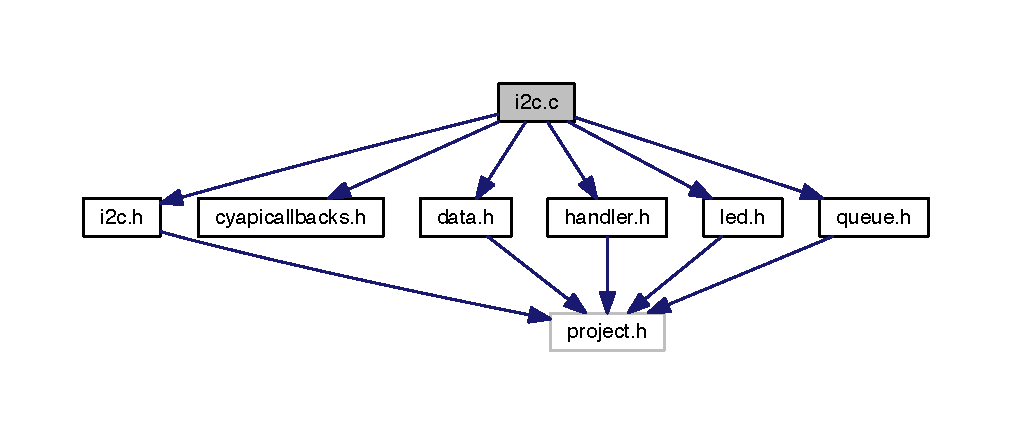
\includegraphics[width=350pt]{d6/d4e/i2c_8c__incl}
\end{center}
\end{figure}


\subsubsection{Detaljeret beskrivelse}
\hyperlink{class_i2_c}{I2C} modul. 

Håndter kommunikation via I2\+C-\/busset \begin{DoxyAuthor}{Forfatter}
Jeppe Stærk Antonsen (\href{mailto:201271201@uni.au.dk}{\tt 201271201@uni.\+au.\+dk}) 
\end{DoxyAuthor}

\hypertarget{i2c_8h}{}\subsection{i2c.\+h filreference}
\label{i2c_8h}\index{i2c.\+h@{i2c.\+h}}


\hyperlink{class_i2_c}{I2C} modul.  


{\ttfamily \#include $<$project.\+h$>$}\\*
Inklusions-\/afhængighedsgraf for i2c.\+h\+:\nopagebreak
\begin{figure}[H]
\begin{center}
\leavevmode
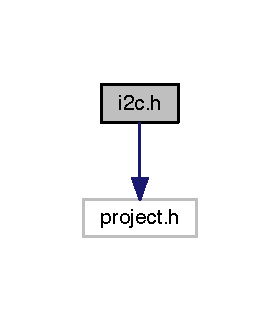
\includegraphics[width=134pt]{de/d0d/i2c_8h__incl}
\end{center}
\end{figure}
Denne graf viser, hvilke filer der direkte eller indirekte inkluderer denne fil\+:\nopagebreak
\begin{figure}[H]
\begin{center}
\leavevmode
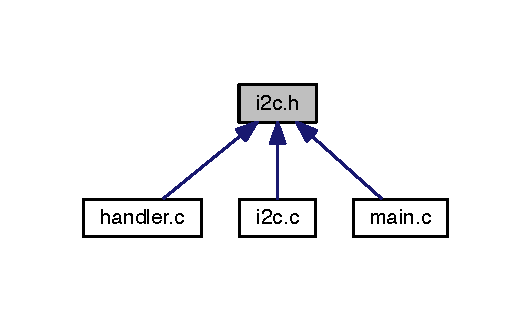
\includegraphics[width=255pt]{d3/df7/i2c_8h__dep__incl}
\end{center}
\end{figure}
\subsubsection*{\#Defines}
\begin{DoxyCompactItemize}
\item 
\#define \hyperlink{i2c_8h_a2c70db7df8defae29c1912d84aaee3dc}{P\+So\+C\+\_\+\+XY}~(0x08u)
\item 
\#define \hyperlink{i2c_8h_aa72315d85eb390444fdd96475c6aa1f4}{P\+So\+C\+\_\+Z}~(0x09u)
\item 
\#define \hyperlink{i2c_8h_adc44ca05813864518773ea6f3543816c}{P\+So\+C\+\_\+\+Sensor}~(0x10u)
\item 
\#define \hyperlink{i2c_8h_a6458dbf193a0eef0470fc1b08400bfcd}{I2\+C\+\_\+\+B\+U\+F\+F\+E\+R\+\_\+\+S\+I\+ZE}~(4u)
\item 
\#define \hyperlink{i2c_8h_a8c24abf58121f3c16b5f687cc2946cd1}{I2\+C\+\_\+\+P\+A\+C\+K\+E\+T\+\_\+\+S\+I\+ZE}~(4u)
\item 
\#define \hyperlink{i2c_8h_a1207f4b2c3692b1a344f0013da629310}{I2\+C\+\_\+\+P\+A\+C\+K\+E\+T\+\_\+\+S\+O\+P\+\_\+\+P\+OS}~(0u)
\item 
\#define \hyperlink{i2c_8h_ac13fcfeded7dc2d82fa4734456f3761f}{I2\+C\+\_\+\+P\+A\+C\+K\+E\+T\+\_\+\+C\+M\+D\+\_\+\+P\+OS}~(1u)
\item 
\#define \hyperlink{i2c_8h_a68506c3651f015716bb2c135e8e7b972}{I2\+C\+\_\+\+P\+A\+C\+K\+E\+T\+\_\+\+V\+A\+L\+\_\+\+P\+OS}~(2u)
\item 
\#define \hyperlink{i2c_8h_a940f0ea8103872c7ba81b9dc0f121feb}{I2\+C\+\_\+\+P\+A\+C\+K\+E\+T\+\_\+\+E\+O\+P\+\_\+\+P\+OS}~(3u)
\item 
\#define \hyperlink{i2c_8h_a52bb5b964361ed2f1b18df32c5b8f2c5}{I2\+C\+\_\+\+P\+A\+C\+K\+E\+T\+\_\+\+S\+OP}~(0x\+B\+Eu)
\item 
\#define \hyperlink{i2c_8h_a62b4ae6e51a3d0da47f5165165cdbc0a}{I2\+C\+\_\+\+P\+A\+C\+K\+E\+T\+\_\+\+E\+OP}~(0x\+E\+Fu)
\item 
\#define \hyperlink{i2c_8h_a7f8f53679384fa228bf06779cc168cfd}{I2\+C\+\_\+\+S\+T\+S\+\_\+\+C\+M\+D\+\_\+\+D\+O\+NE}~(0x\+A\+Au)
\item 
\#define \hyperlink{i2c_8h_aee0adbd7dcb13e95337369b7342a27e3}{I2\+C\+\_\+\+S\+T\+S\+\_\+\+C\+M\+D\+\_\+\+F\+A\+IL}~(0x\+E\+Eu)
\end{DoxyCompactItemize}
\subsubsection*{Funktioner}
\begin{DoxyCompactItemize}
\item 
void \hyperlink{i2c_8h_a5730d9445429351b9f750084c5cb5aae}{i2c\+\_\+init} (void)
\item 
void \hyperlink{i2c_8h_a0e13c9c7d87ebdb3680495a787f68d29}{i2c\+\_\+set\+Packet} (uint8 i2c\+Addr, uint8 i2c\+Cmd, uint8 i2c\+Val)
\item 
void \hyperlink{i2c_8h_afd44ef28b428b7ec2cffb38c97340251}{i2c\+\_\+get\+Packet} (uint8 i2c\+Addr, uint8 i2c\+Cmd, uint8 $\ast$i2c\+Val)
\end{DoxyCompactItemize}


\subsubsection{Detaljeret beskrivelse}
\hyperlink{class_i2_c}{I2C} modul. 

Håndter kommunikation via I2\+C-\/busset. \begin{DoxyAuthor}{Forfatter}
Jeppe Stærk Antonsen (\href{mailto:201271201@uni.au.dk}{\tt 201271201@uni.\+au.\+dk}) 
\end{DoxyAuthor}


\subsubsection{\#Define-\/dokumentation}
\index{i2c.\+h@{i2c.\+h}!I2\+C\+\_\+\+B\+U\+F\+F\+E\+R\+\_\+\+S\+I\+ZE@{I2\+C\+\_\+\+B\+U\+F\+F\+E\+R\+\_\+\+S\+I\+ZE}}
\index{I2\+C\+\_\+\+B\+U\+F\+F\+E\+R\+\_\+\+S\+I\+ZE@{I2\+C\+\_\+\+B\+U\+F\+F\+E\+R\+\_\+\+S\+I\+ZE}!i2c.\+h@{i2c.\+h}}
\paragraph[{\texorpdfstring{I2\+C\+\_\+\+B\+U\+F\+F\+E\+R\+\_\+\+S\+I\+ZE}{I2C_BUFFER_SIZE}}]{\setlength{\rightskip}{0pt plus 5cm}\#define I2\+C\+\_\+\+B\+U\+F\+F\+E\+R\+\_\+\+S\+I\+ZE~(4u)}\hypertarget{i2c_8h_a6458dbf193a0eef0470fc1b08400bfcd}{}\label{i2c_8h_a6458dbf193a0eef0470fc1b08400bfcd}


Defineret på linje 42 i filen i2c.\+h.



Refereret til af I2\+C\+::i2c\+\_\+rx() og I2\+C\+::i2c\+\_\+tx().

\index{i2c.\+h@{i2c.\+h}!I2\+C\+\_\+\+P\+A\+C\+K\+E\+T\+\_\+\+C\+M\+D\+\_\+\+P\+OS@{I2\+C\+\_\+\+P\+A\+C\+K\+E\+T\+\_\+\+C\+M\+D\+\_\+\+P\+OS}}
\index{I2\+C\+\_\+\+P\+A\+C\+K\+E\+T\+\_\+\+C\+M\+D\+\_\+\+P\+OS@{I2\+C\+\_\+\+P\+A\+C\+K\+E\+T\+\_\+\+C\+M\+D\+\_\+\+P\+OS}!i2c.\+h@{i2c.\+h}}
\paragraph[{\texorpdfstring{I2\+C\+\_\+\+P\+A\+C\+K\+E\+T\+\_\+\+C\+M\+D\+\_\+\+P\+OS}{I2C_PACKET_CMD_POS}}]{\setlength{\rightskip}{0pt plus 5cm}\#define I2\+C\+\_\+\+P\+A\+C\+K\+E\+T\+\_\+\+C\+M\+D\+\_\+\+P\+OS~(1u)}\hypertarget{i2c_8h_ac13fcfeded7dc2d82fa4734456f3761f}{}\label{i2c_8h_ac13fcfeded7dc2d82fa4734456f3761f}


Defineret på linje 47 i filen i2c.\+h.



Refereret til af I2\+C\+::i2c\+\_\+rx() og I2\+C\+::i2c\+\_\+tx().

\index{i2c.\+h@{i2c.\+h}!I2\+C\+\_\+\+P\+A\+C\+K\+E\+T\+\_\+\+E\+OP@{I2\+C\+\_\+\+P\+A\+C\+K\+E\+T\+\_\+\+E\+OP}}
\index{I2\+C\+\_\+\+P\+A\+C\+K\+E\+T\+\_\+\+E\+OP@{I2\+C\+\_\+\+P\+A\+C\+K\+E\+T\+\_\+\+E\+OP}!i2c.\+h@{i2c.\+h}}
\paragraph[{\texorpdfstring{I2\+C\+\_\+\+P\+A\+C\+K\+E\+T\+\_\+\+E\+OP}{I2C_PACKET_EOP}}]{\setlength{\rightskip}{0pt plus 5cm}\#define I2\+C\+\_\+\+P\+A\+C\+K\+E\+T\+\_\+\+E\+OP~(0x\+E\+Fu)}\hypertarget{i2c_8h_a62b4ae6e51a3d0da47f5165165cdbc0a}{}\label{i2c_8h_a62b4ae6e51a3d0da47f5165165cdbc0a}


Defineret på linje 53 i filen i2c.\+h.



Refereret til af I2\+C\+::i2c\+\_\+rx() og I2\+C\+::i2c\+\_\+tx().

\index{i2c.\+h@{i2c.\+h}!I2\+C\+\_\+\+P\+A\+C\+K\+E\+T\+\_\+\+E\+O\+P\+\_\+\+P\+OS@{I2\+C\+\_\+\+P\+A\+C\+K\+E\+T\+\_\+\+E\+O\+P\+\_\+\+P\+OS}}
\index{I2\+C\+\_\+\+P\+A\+C\+K\+E\+T\+\_\+\+E\+O\+P\+\_\+\+P\+OS@{I2\+C\+\_\+\+P\+A\+C\+K\+E\+T\+\_\+\+E\+O\+P\+\_\+\+P\+OS}!i2c.\+h@{i2c.\+h}}
\paragraph[{\texorpdfstring{I2\+C\+\_\+\+P\+A\+C\+K\+E\+T\+\_\+\+E\+O\+P\+\_\+\+P\+OS}{I2C_PACKET_EOP_POS}}]{\setlength{\rightskip}{0pt plus 5cm}\#define I2\+C\+\_\+\+P\+A\+C\+K\+E\+T\+\_\+\+E\+O\+P\+\_\+\+P\+OS~(3u)}\hypertarget{i2c_8h_a940f0ea8103872c7ba81b9dc0f121feb}{}\label{i2c_8h_a940f0ea8103872c7ba81b9dc0f121feb}


Defineret på linje 49 i filen i2c.\+h.



Refereret til af I2\+C\+::i2c\+\_\+rx() og I2\+C\+::i2c\+\_\+tx().

\index{i2c.\+h@{i2c.\+h}!I2\+C\+\_\+\+P\+A\+C\+K\+E\+T\+\_\+\+S\+I\+ZE@{I2\+C\+\_\+\+P\+A\+C\+K\+E\+T\+\_\+\+S\+I\+ZE}}
\index{I2\+C\+\_\+\+P\+A\+C\+K\+E\+T\+\_\+\+S\+I\+ZE@{I2\+C\+\_\+\+P\+A\+C\+K\+E\+T\+\_\+\+S\+I\+ZE}!i2c.\+h@{i2c.\+h}}
\paragraph[{\texorpdfstring{I2\+C\+\_\+\+P\+A\+C\+K\+E\+T\+\_\+\+S\+I\+ZE}{I2C_PACKET_SIZE}}]{\setlength{\rightskip}{0pt plus 5cm}\#define I2\+C\+\_\+\+P\+A\+C\+K\+E\+T\+\_\+\+S\+I\+ZE~(4u)}\hypertarget{i2c_8h_a8c24abf58121f3c16b5f687cc2946cd1}{}\label{i2c_8h_a8c24abf58121f3c16b5f687cc2946cd1}


Defineret på linje 43 i filen i2c.\+h.



Refereret til af I2\+C\+::i2c\+\_\+rx() og I2\+C\+::i2c\+\_\+tx().

\index{i2c.\+h@{i2c.\+h}!I2\+C\+\_\+\+P\+A\+C\+K\+E\+T\+\_\+\+S\+OP@{I2\+C\+\_\+\+P\+A\+C\+K\+E\+T\+\_\+\+S\+OP}}
\index{I2\+C\+\_\+\+P\+A\+C\+K\+E\+T\+\_\+\+S\+OP@{I2\+C\+\_\+\+P\+A\+C\+K\+E\+T\+\_\+\+S\+OP}!i2c.\+h@{i2c.\+h}}
\paragraph[{\texorpdfstring{I2\+C\+\_\+\+P\+A\+C\+K\+E\+T\+\_\+\+S\+OP}{I2C_PACKET_SOP}}]{\setlength{\rightskip}{0pt plus 5cm}\#define I2\+C\+\_\+\+P\+A\+C\+K\+E\+T\+\_\+\+S\+OP~(0x\+B\+Eu)}\hypertarget{i2c_8h_a52bb5b964361ed2f1b18df32c5b8f2c5}{}\label{i2c_8h_a52bb5b964361ed2f1b18df32c5b8f2c5}


Defineret på linje 52 i filen i2c.\+h.



Refereret til af I2\+C\+::i2c\+\_\+rx() og I2\+C\+::i2c\+\_\+tx().

\index{i2c.\+h@{i2c.\+h}!I2\+C\+\_\+\+P\+A\+C\+K\+E\+T\+\_\+\+S\+O\+P\+\_\+\+P\+OS@{I2\+C\+\_\+\+P\+A\+C\+K\+E\+T\+\_\+\+S\+O\+P\+\_\+\+P\+OS}}
\index{I2\+C\+\_\+\+P\+A\+C\+K\+E\+T\+\_\+\+S\+O\+P\+\_\+\+P\+OS@{I2\+C\+\_\+\+P\+A\+C\+K\+E\+T\+\_\+\+S\+O\+P\+\_\+\+P\+OS}!i2c.\+h@{i2c.\+h}}
\paragraph[{\texorpdfstring{I2\+C\+\_\+\+P\+A\+C\+K\+E\+T\+\_\+\+S\+O\+P\+\_\+\+P\+OS}{I2C_PACKET_SOP_POS}}]{\setlength{\rightskip}{0pt plus 5cm}\#define I2\+C\+\_\+\+P\+A\+C\+K\+E\+T\+\_\+\+S\+O\+P\+\_\+\+P\+OS~(0u)}\hypertarget{i2c_8h_a1207f4b2c3692b1a344f0013da629310}{}\label{i2c_8h_a1207f4b2c3692b1a344f0013da629310}


Defineret på linje 46 i filen i2c.\+h.



Refereret til af I2\+C\+::i2c\+\_\+rx() og I2\+C\+::i2c\+\_\+tx().

\index{i2c.\+h@{i2c.\+h}!I2\+C\+\_\+\+P\+A\+C\+K\+E\+T\+\_\+\+V\+A\+L\+\_\+\+P\+OS@{I2\+C\+\_\+\+P\+A\+C\+K\+E\+T\+\_\+\+V\+A\+L\+\_\+\+P\+OS}}
\index{I2\+C\+\_\+\+P\+A\+C\+K\+E\+T\+\_\+\+V\+A\+L\+\_\+\+P\+OS@{I2\+C\+\_\+\+P\+A\+C\+K\+E\+T\+\_\+\+V\+A\+L\+\_\+\+P\+OS}!i2c.\+h@{i2c.\+h}}
\paragraph[{\texorpdfstring{I2\+C\+\_\+\+P\+A\+C\+K\+E\+T\+\_\+\+V\+A\+L\+\_\+\+P\+OS}{I2C_PACKET_VAL_POS}}]{\setlength{\rightskip}{0pt plus 5cm}\#define I2\+C\+\_\+\+P\+A\+C\+K\+E\+T\+\_\+\+V\+A\+L\+\_\+\+P\+OS~(2u)}\hypertarget{i2c_8h_a68506c3651f015716bb2c135e8e7b972}{}\label{i2c_8h_a68506c3651f015716bb2c135e8e7b972}


Defineret på linje 48 i filen i2c.\+h.



Refereret til af I2\+C\+::i2c\+\_\+rx() og I2\+C\+::i2c\+\_\+tx().

\index{i2c.\+h@{i2c.\+h}!I2\+C\+\_\+\+S\+T\+S\+\_\+\+C\+M\+D\+\_\+\+D\+O\+NE@{I2\+C\+\_\+\+S\+T\+S\+\_\+\+C\+M\+D\+\_\+\+D\+O\+NE}}
\index{I2\+C\+\_\+\+S\+T\+S\+\_\+\+C\+M\+D\+\_\+\+D\+O\+NE@{I2\+C\+\_\+\+S\+T\+S\+\_\+\+C\+M\+D\+\_\+\+D\+O\+NE}!i2c.\+h@{i2c.\+h}}
\paragraph[{\texorpdfstring{I2\+C\+\_\+\+S\+T\+S\+\_\+\+C\+M\+D\+\_\+\+D\+O\+NE}{I2C_STS_CMD_DONE}}]{\setlength{\rightskip}{0pt plus 5cm}\#define I2\+C\+\_\+\+S\+T\+S\+\_\+\+C\+M\+D\+\_\+\+D\+O\+NE~(0x\+A\+Au)}\hypertarget{i2c_8h_a7f8f53679384fa228bf06779cc168cfd}{}\label{i2c_8h_a7f8f53679384fa228bf06779cc168cfd}


Defineret på linje 56 i filen i2c.\+h.



Refereret til af I2\+C\+::i2c\+\_\+get\+Packet(), I2\+C\+::i2c\+\_\+set\+Packet() og I2\+C\+::i2c\+\_\+tx().

\index{i2c.\+h@{i2c.\+h}!I2\+C\+\_\+\+S\+T\+S\+\_\+\+C\+M\+D\+\_\+\+F\+A\+IL@{I2\+C\+\_\+\+S\+T\+S\+\_\+\+C\+M\+D\+\_\+\+F\+A\+IL}}
\index{I2\+C\+\_\+\+S\+T\+S\+\_\+\+C\+M\+D\+\_\+\+F\+A\+IL@{I2\+C\+\_\+\+S\+T\+S\+\_\+\+C\+M\+D\+\_\+\+F\+A\+IL}!i2c.\+h@{i2c.\+h}}
\paragraph[{\texorpdfstring{I2\+C\+\_\+\+S\+T\+S\+\_\+\+C\+M\+D\+\_\+\+F\+A\+IL}{I2C_STS_CMD_FAIL}}]{\setlength{\rightskip}{0pt plus 5cm}\#define I2\+C\+\_\+\+S\+T\+S\+\_\+\+C\+M\+D\+\_\+\+F\+A\+IL~(0x\+E\+Eu)}\hypertarget{i2c_8h_aee0adbd7dcb13e95337369b7342a27e3}{}\label{i2c_8h_aee0adbd7dcb13e95337369b7342a27e3}


Defineret på linje 57 i filen i2c.\+h.



Refereret til af I2\+C\+::i2c\+\_\+rx() og I2\+C\+::i2c\+\_\+tx().

\index{i2c.\+h@{i2c.\+h}!P\+So\+C\+\_\+\+Sensor@{P\+So\+C\+\_\+\+Sensor}}
\index{P\+So\+C\+\_\+\+Sensor@{P\+So\+C\+\_\+\+Sensor}!i2c.\+h@{i2c.\+h}}
\paragraph[{\texorpdfstring{P\+So\+C\+\_\+\+Sensor}{PSoC_Sensor}}]{\setlength{\rightskip}{0pt plus 5cm}\#define P\+So\+C\+\_\+\+Sensor~(0x10u)}\hypertarget{i2c_8h_adc44ca05813864518773ea6f3543816c}{}\label{i2c_8h_adc44ca05813864518773ea6f3543816c}


Defineret på linje 39 i filen i2c.\+h.



Refereret til af Handler\+::handler().

\index{i2c.\+h@{i2c.\+h}!P\+So\+C\+\_\+\+XY@{P\+So\+C\+\_\+\+XY}}
\index{P\+So\+C\+\_\+\+XY@{P\+So\+C\+\_\+\+XY}!i2c.\+h@{i2c.\+h}}
\paragraph[{\texorpdfstring{P\+So\+C\+\_\+\+XY}{PSoC_XY}}]{\setlength{\rightskip}{0pt plus 5cm}\#define P\+So\+C\+\_\+\+XY~(0x08u)}\hypertarget{i2c_8h_a2c70db7df8defae29c1912d84aaee3dc}{}\label{i2c_8h_a2c70db7df8defae29c1912d84aaee3dc}


Defineret på linje 37 i filen i2c.\+h.



Refereret til af Handler\+::handler().

\index{i2c.\+h@{i2c.\+h}!P\+So\+C\+\_\+Z@{P\+So\+C\+\_\+Z}}
\index{P\+So\+C\+\_\+Z@{P\+So\+C\+\_\+Z}!i2c.\+h@{i2c.\+h}}
\paragraph[{\texorpdfstring{P\+So\+C\+\_\+Z}{PSoC_Z}}]{\setlength{\rightskip}{0pt plus 5cm}\#define P\+So\+C\+\_\+Z~(0x09u)}\hypertarget{i2c_8h_aa72315d85eb390444fdd96475c6aa1f4}{}\label{i2c_8h_aa72315d85eb390444fdd96475c6aa1f4}


Defineret på linje 38 i filen i2c.\+h.



Refereret til af Handler\+::handler().



\subsubsection{Funktions-\/dokumentation}
\index{i2c.\+h@{i2c.\+h}!i2c\+\_\+get\+Packet@{i2c\+\_\+get\+Packet}}
\index{i2c\+\_\+get\+Packet@{i2c\+\_\+get\+Packet}!i2c.\+h@{i2c.\+h}}
\paragraph[{\texorpdfstring{i2c\+\_\+get\+Packet(uint8 i2c\+Addr, uint8 i2c\+Cmd, uint8 $\ast$i2c\+Val)}{i2c_getPacket(uint8 i2cAddr, uint8 i2cCmd, uint8 *i2cVal)}}]{\setlength{\rightskip}{0pt plus 5cm}void i2c\+\_\+get\+Packet (
\begin{DoxyParamCaption}
\item[{uint8}]{i2c\+Addr, }
\item[{uint8}]{i2c\+Cmd, }
\item[{uint8 $\ast$}]{i2c\+Val}
\end{DoxyParamCaption}
)}\hypertarget{i2c_8h_afd44ef28b428b7ec2cffb38c97340251}{}\label{i2c_8h_afd44ef28b428b7ec2cffb38c97340251}
\index{i2c.\+h@{i2c.\+h}!i2c\+\_\+init@{i2c\+\_\+init}}
\index{i2c\+\_\+init@{i2c\+\_\+init}!i2c.\+h@{i2c.\+h}}
\paragraph[{\texorpdfstring{i2c\+\_\+init(void)}{i2c_init(void)}}]{\setlength{\rightskip}{0pt plus 5cm}void i2c\+\_\+init (
\begin{DoxyParamCaption}
\item[{void}]{}
\end{DoxyParamCaption}
)}\hypertarget{i2c_8h_a5730d9445429351b9f750084c5cb5aae}{}\label{i2c_8h_a5730d9445429351b9f750084c5cb5aae}
\index{i2c.\+h@{i2c.\+h}!i2c\+\_\+set\+Packet@{i2c\+\_\+set\+Packet}}
\index{i2c\+\_\+set\+Packet@{i2c\+\_\+set\+Packet}!i2c.\+h@{i2c.\+h}}
\paragraph[{\texorpdfstring{i2c\+\_\+set\+Packet(uint8 i2c\+Addr, uint8 i2c\+Cmd, uint8 i2c\+Val)}{i2c_setPacket(uint8 i2cAddr, uint8 i2cCmd, uint8 i2cVal)}}]{\setlength{\rightskip}{0pt plus 5cm}void i2c\+\_\+set\+Packet (
\begin{DoxyParamCaption}
\item[{uint8}]{i2c\+Addr, }
\item[{uint8}]{i2c\+Cmd, }
\item[{uint8}]{i2c\+Val}
\end{DoxyParamCaption}
)}\hypertarget{i2c_8h_a0e13c9c7d87ebdb3680495a787f68d29}{}\label{i2c_8h_a0e13c9c7d87ebdb3680495a787f68d29}

\hypertarget{led_8c}{}\subsection{led.\+c filreference}
\label{led_8c}\index{led.\+c@{led.\+c}}


\hyperlink{class_l_e_d}{L\+ED} modul.  


{\ttfamily \#include \char`\"{}led.\+h\char`\"{}}\\*
Inklusions-\/afhængighedsgraf for led.\+c\+:\nopagebreak
\begin{figure}[H]
\begin{center}
\leavevmode
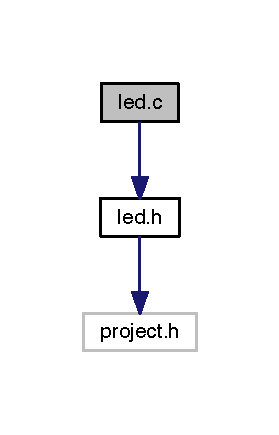
\includegraphics[width=134pt]{df/d0a/led_8c__incl}
\end{center}
\end{figure}


\subsubsection{Detaljeret beskrivelse}
\hyperlink{class_l_e_d}{L\+ED} modul. 

Håndtere P\+SoC\textquotesingle{}ens røde, grønne og blå led. \begin{DoxyAuthor}{Forfatter}
Casper Dieu Le (\href{mailto:201370338@uni.au.dk}{\tt 201370338@uni.\+au.\+dk}) 

Kasper Hinkler Uldbjerg (\href{mailto:201370281@uni.au.dk}{\tt 201370281@uni.\+au.\+dk}) 

Jeppe Stærk Antonsen (\href{mailto:201271201@uni.au.dk}{\tt 201271201@uni.\+au.\+dk}) 
\end{DoxyAuthor}

\hypertarget{led_8h}{}\subsection{led.\+h filreference}
\label{led_8h}\index{led.\+h@{led.\+h}}


\hyperlink{class_l_e_d}{L\+ED} modul.  


{\ttfamily \#include $<$project.\+h$>$}\\*
Inklusions-\/afhængighedsgraf for led.\+h\+:
\nopagebreak
\begin{figure}[H]
\begin{center}
\leavevmode
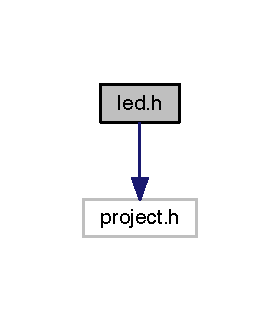
\includegraphics[width=134pt]{d6/d11/led_8h__incl}
\end{center}
\end{figure}
Denne graf viser, hvilke filer der direkte eller indirekte inkluderer denne fil\+:
\nopagebreak
\begin{figure}[H]
\begin{center}
\leavevmode
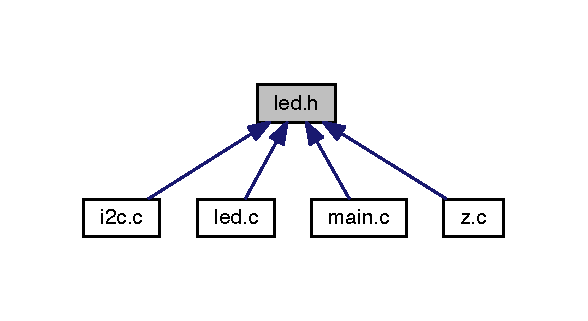
\includegraphics[width=235pt]{d6/dde/led_8h__dep__incl}
\end{center}
\end{figure}
\subsubsection*{\#Defines}
\begin{DoxyCompactItemize}
\item 
\#define \hyperlink{led_8h_af2e697ac60e05813d45ea2c9c9e79c25}{L\+E\+D\+\_\+\+ON}~(0u)
\item 
\#define \hyperlink{led_8h_a80700bb63bd56ebabbb4728aa433fd29}{L\+E\+D\+\_\+\+O\+FF}~(1u)
\end{DoxyCompactItemize}
\subsubsection*{Funktioner}
\begin{DoxyCompactItemize}
\item 
void \hyperlink{led_8h_a1d8e725e3829da99c1d027ba0a2ce57a}{set\+Led} (uint8 red, uint8 green, uint8 blue, uint8 delay)
\end{DoxyCompactItemize}


\subsubsection{Detaljeret beskrivelse}
\hyperlink{class_l_e_d}{L\+ED} modul. 

Håndtere P\+SoC\textquotesingle{}ens røde, grønne og blå led. \begin{DoxyAuthor}{Forfatter}
Jeppe Stærk Antonsen (\href{mailto:201271201@uni.au.dk}{\tt 201271201@uni.\+au.\+dk}) 
\end{DoxyAuthor}


\subsubsection{\#Define-\/dokumentation}
\index{led.\+h@{led.\+h}!L\+E\+D\+\_\+\+O\+FF@{L\+E\+D\+\_\+\+O\+FF}}
\index{L\+E\+D\+\_\+\+O\+FF@{L\+E\+D\+\_\+\+O\+FF}!led.\+h@{led.\+h}}
\paragraph[{\texorpdfstring{L\+E\+D\+\_\+\+O\+FF}{LED_OFF}}]{\setlength{\rightskip}{0pt plus 5cm}\#define L\+E\+D\+\_\+\+O\+FF~(1u)}\hypertarget{led_8h_a80700bb63bd56ebabbb4728aa433fd29}{}\label{led_8h_a80700bb63bd56ebabbb4728aa433fd29}


Defineret på linje 37 i filen led.\+h.



Refereret til af L\+E\+D\+::set\+Led().

\index{led.\+h@{led.\+h}!L\+E\+D\+\_\+\+ON@{L\+E\+D\+\_\+\+ON}}
\index{L\+E\+D\+\_\+\+ON@{L\+E\+D\+\_\+\+ON}!led.\+h@{led.\+h}}
\paragraph[{\texorpdfstring{L\+E\+D\+\_\+\+ON}{LED_ON}}]{\setlength{\rightskip}{0pt plus 5cm}\#define L\+E\+D\+\_\+\+ON~(0u)}\hypertarget{led_8h_af2e697ac60e05813d45ea2c9c9e79c25}{}\label{led_8h_af2e697ac60e05813d45ea2c9c9e79c25}


Defineret på linje 36 i filen led.\+h.



Refereret til af L\+E\+D\+::set\+Led().



\subsubsection{Funktions-\/dokumentation}
\index{led.\+h@{led.\+h}!set\+Led@{set\+Led}}
\index{set\+Led@{set\+Led}!led.\+h@{led.\+h}}
\paragraph[{\texorpdfstring{set\+Led(uint8 red, uint8 green, uint8 blue, uint8 delay)}{setLed(uint8 red, uint8 green, uint8 blue, uint8 delay)}}]{\setlength{\rightskip}{0pt plus 5cm}void set\+Led (
\begin{DoxyParamCaption}
\item[{uint8}]{red, }
\item[{uint8}]{green, }
\item[{uint8}]{blue, }
\item[{uint8}]{delay}
\end{DoxyParamCaption}
)}\hypertarget{led_8h_a1d8e725e3829da99c1d027ba0a2ce57a}{}\label{led_8h_a1d8e725e3829da99c1d027ba0a2ce57a}

\hypertarget{main_8c}{}\subsection{main.\+c filreference}
\label{main_8c}\index{main.\+c@{main.\+c}}


Hovedprogram.  


{\ttfamily \#include $<$project.\+h$>$}\\*
{\ttfamily \#include \char`\"{}data.\+h\char`\"{}}\\*
{\ttfamily \#include \char`\"{}handler.\+h\char`\"{}}\\*
{\ttfamily \#include \char`\"{}i2c.\+h\char`\"{}}\\*
{\ttfamily \#include \char`\"{}led.\+h\char`\"{}}\\*
{\ttfamily \#include \char`\"{}queue.\+h\char`\"{}}\\*
{\ttfamily \#include \char`\"{}xy.\+h\char`\"{}}\\*
Inklusions-\/afhængighedsgraf for main.\+c\+:
\nopagebreak
\begin{figure}[H]
\begin{center}
\leavevmode
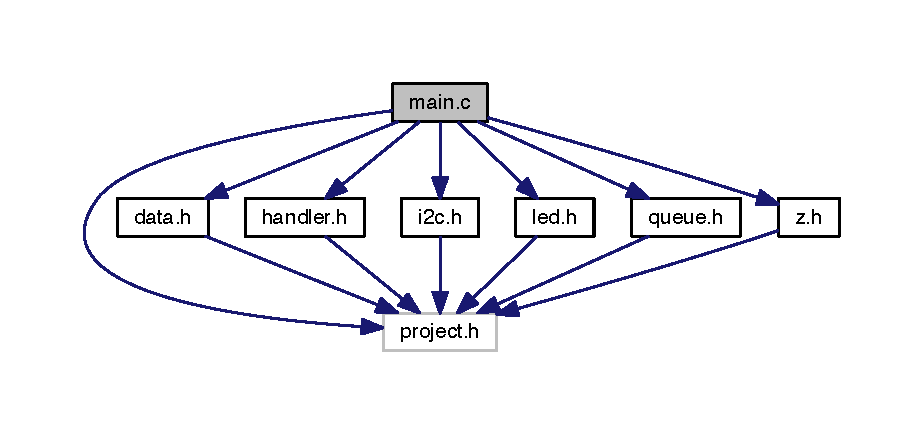
\includegraphics[width=350pt]{d4/d10/main_8c__incl}
\end{center}
\end{figure}
\subsubsection*{Funktioner}
\begin{DoxyCompactItemize}
\item 
int \hyperlink{main_8c_ae66f6b31b5ad750f1fe042a706a4e3d4}{main} ()
\end{DoxyCompactItemize}


\subsubsection{Detaljeret beskrivelse}
Hovedprogram. 

Intilizere modulerne og køre derefter i loop hvor der bliver kontrolieret om der er nogle actions i køen der skal håndteres af handleren. \begin{DoxyAuthor}{Forfatter}
Casper Dieu Le (\href{mailto:201370338@uni.au.dk}{\tt 201370338@uni.\+au.\+dk}) 

Kasper Hinkler Uldbjerg (\href{mailto:201370281@uni.au.dk}{\tt 201370281@uni.\+au.\+dk}) 

Jeppe Stærk (\href{mailto:201271201@uni.au.dk}{\tt 201271201@uni.\+au.\+dk}) 
\end{DoxyAuthor}


\subsubsection{Funktions-\/dokumentation}
\index{main.\+c@{main.\+c}!main@{main}}
\index{main@{main}!main.\+c@{main.\+c}}
\paragraph[{\texorpdfstring{main()}{main()}}]{\setlength{\rightskip}{0pt plus 5cm}int main (
\begin{DoxyParamCaption}
{}
\end{DoxyParamCaption}
)}\hypertarget{main_8c_ae66f6b31b5ad750f1fe042a706a4e3d4}{}\label{main_8c_ae66f6b31b5ad750f1fe042a706a4e3d4}


Defineret på linje 17 i filen main.\+c.



Indeholder referencer til X\+Y\+::calibrate\+X(), X\+Y\+::calibrate\+Y(), Data\+::data\+\_\+init(), Queue\+::front\+Queue(), Handler\+::handler(), I2\+C\+::i2c\+\_\+init(), I2\+C\+::i2c\+\_\+tx(), Queue\+::is\+Empty\+Queue(), Queue\+::pop\+Queue(), Queue\+::queue\+\_\+init(), L\+E\+D\+::set\+Led(), X\+Y\+::xy\+\_\+init() og X\+Y\+::xy\+\_\+start().


\begin{DoxyCode}
18 \{
19   CyGlobalIntEnable;
20   
21   \hyperlink{class_data_adf37c815716edf228a3cbb4564290275}{data\_init}();
22   \hyperlink{class_queue_a4e0a3758d721506e7729f4d074a280ff}{queue\_init}(6u);
23   \hyperlink{class_x_y_aaf6d50e1866014a76b1b15325d2dba4b}{xy\_init}();
24   \hyperlink{class_i2_c_a64303230bf4843297e7ac37ac236ca04}{i2c\_init}();
25   
26   DEBUG\_PutCRLF();
27   DEBUG\_PutString(\textcolor{stringliteral}{"===== Initializing PSoC XY ====="});
28   DEBUG\_PutCRLF();
29   
30   \hyperlink{class_l_e_d_a1d8e725e3829da99c1d027ba0a2ce57a}{setLed}(0,1,0,0);
31   CyDelay(100);
32   \hyperlink{class_l_e_d_a1d8e725e3829da99c1d027ba0a2ce57a}{setLed}(0,0,0,0);
33   
34   \hyperlink{class_x_y_a47c6cc7fae92395e4d1231428c7070d4}{xy\_start}();
35   
36   \textcolor{keywordflow}{for}(;;)
37   \{
38     \textcolor{keywordflow}{if}(SW2\_Read() == 0u)
39     \{
40       CyDelay(5u);
41       \textcolor{keywordflow}{if}(SW2\_Read() == 0u)
42       \{
43         \hyperlink{class_x_y_a852d7d757cec8e85e0b436969d0ce237}{calibrateX}();
44         \hyperlink{class_x_y_a86751f168bdc352fa109644298829609}{calibrateY}();
45       \}
46       \textcolor{keywordflow}{while}(SW2\_Read() == 0u)
47       \{
48         ; \textcolor{comment}{/* Wait till button released */}
49       \}
50     \}
51     
52     \textcolor{keywordflow}{while}(\hyperlink{class_queue_aafb324c79731abdc228dbf94d86722a3}{isEmptyQueue}() != 1)
53     \{
54       \textcolor{keyword}{struct }\hyperlink{queue_8h_df/d8c/struct_action}{Action} action;
55       action = \hyperlink{class_queue_a49c50ba30a42033068d8d8e6a23c6ca1}{frontQueue}();
56       \hyperlink{class_handler_af5be5b016b862943cd22504490acc8f4}{handler}(action.cmd, action.val);
57       \hyperlink{class_queue_a9ecab9ecdedfc331aed9a0ae63ce193b}{popQueue}();
58     \}
59     \hyperlink{class_i2_c_a3d3187ad377a6ca29b3fac5c809b6012}{i2c\_tx}();
60   \}
61 \}
\end{DoxyCode}


Her er kald-\/grafen for denne funktion\+:
\nopagebreak
\begin{figure}[H]
\begin{center}
\leavevmode
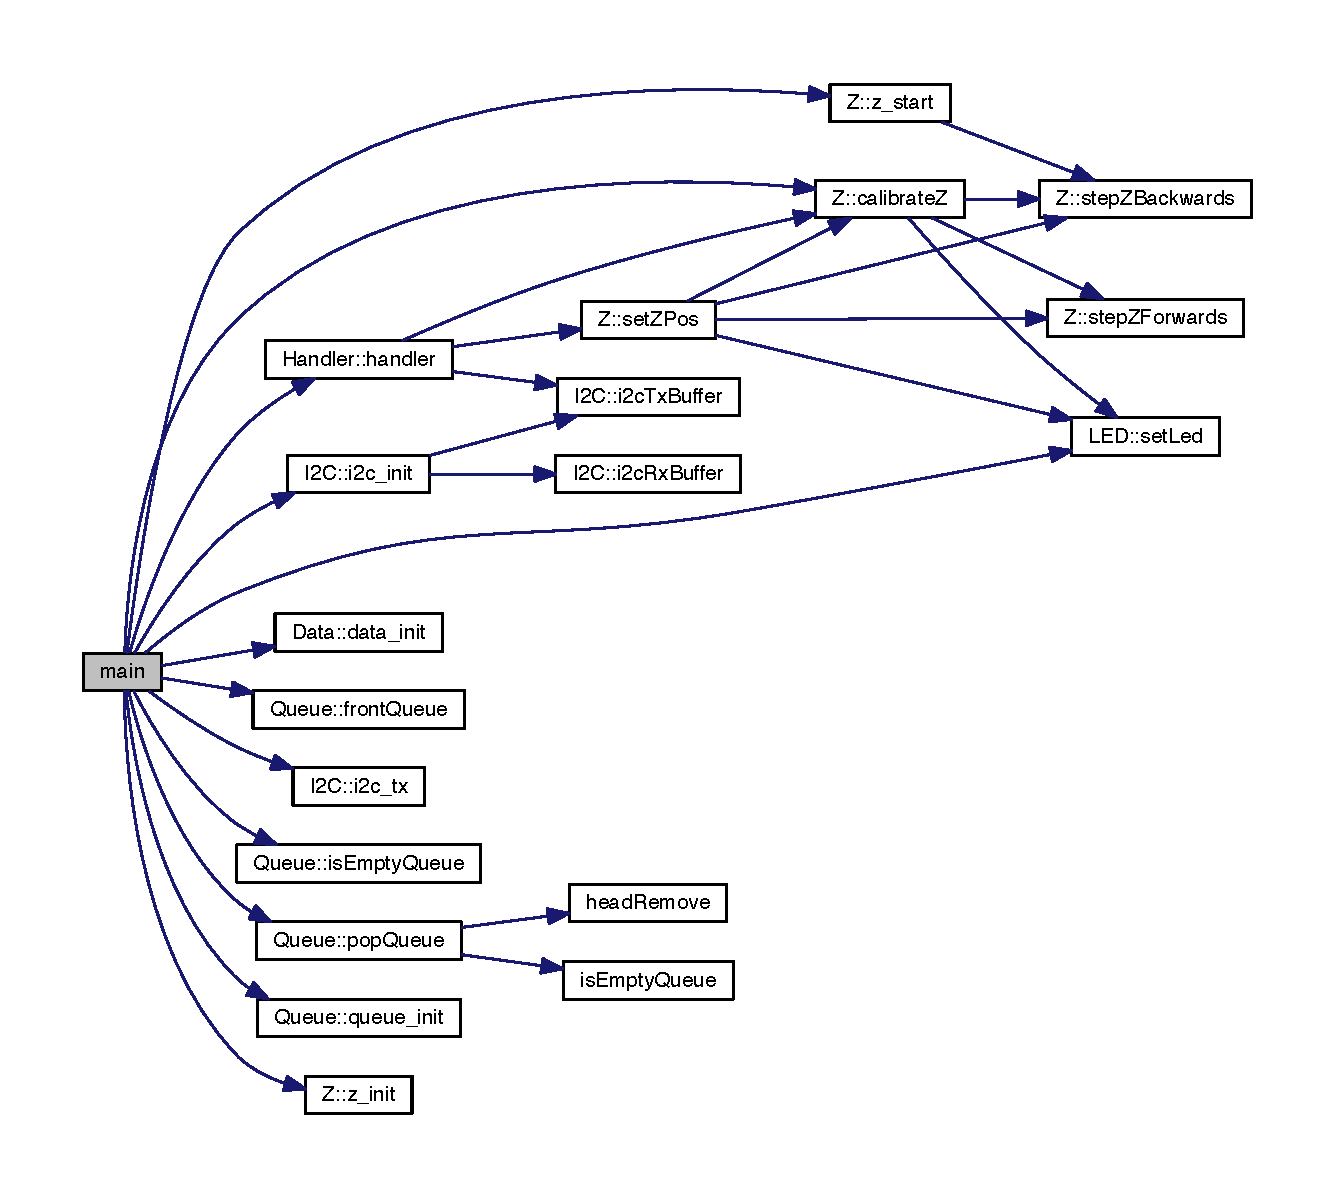
\includegraphics[width=350pt]{d0/d29/main_8c_ae66f6b31b5ad750f1fe042a706a4e3d4_cgraph}
\end{center}
\end{figure}



\hypertarget{queue_8c}{}\subsection{queue.\+c filreference}
\label{queue_8c}\index{queue.\+c@{queue.\+c}}


A queue for incoming commands.  


{\ttfamily \#include \char`\"{}queue.\+h\char`\"{}}\\*
{\ttfamily \#include $<$stdio.\+h$>$}\\*
{\ttfamily \#include $<$stdlib.\+h$>$}\\*
Inklusions-\/afhængighedsgraf for queue.\+c\+:
\nopagebreak
\begin{figure}[H]
\begin{center}
\leavevmode
\includegraphics[width=263pt]{d1/d50/queue_8c__incl}
\end{center}
\end{figure}
\subsubsection*{Datastrukturer}
\begin{DoxyCompactItemize}
\item 
struct \hyperlink{queue_8c_db/d8b/struct_node}{Node}
\begin{DoxyCompactList}\small\item\em Struct to contain a element in the queue.  \hyperlink{queue_8c_db/d8b/struct_node}{Mere...}\end{DoxyCompactList}\end{DoxyCompactItemize}
\subsubsection*{Funktioner}
\begin{DoxyCompactItemize}
\item 
static void \hyperlink{queue_8c_a2607abf0fdd9192a8da3b72245bf593f}{head\+Insert} (struct \hyperlink{queue_8c_db/d8b/struct_node}{Node} $\ast$$\ast$head\+Ptr, const struct \hyperlink{queue_8h_da/d48/struct_data}{Data} data)
\item 
static void \hyperlink{queue_8c_a3f4e77137b39d4f0461d240a5a372917}{head\+Remove} (struct \hyperlink{queue_8c_db/d8b/struct_node}{Node} $\ast$$\ast$head\+Ptr)
\item 
static void \hyperlink{queue_8c_a8e59eeb600ef9f52372bfcb13d1fb6ff}{back\+Insert} (struct \hyperlink{queue_8c_db/d8b/struct_node}{Node} $\ast$$\ast$back\+Ptr, const struct \hyperlink{queue_8h_da/d48/struct_data}{Data} data)
\end{DoxyCompactItemize}


\subsubsection{Detaljeret beskrivelse}
A queue for incoming commands. 



\subsubsection{Datastruktur-\/documentation}
\index{Node@{Node}}\label{struct_node}
\hypertarget{queue_8c_struct_node}{}
\paragraph{struct Node}
Struct to contain a element in the queue. 

\begin{DoxyAuthor}{Forfatter}
Jeppe Stærk (\href{mailto:201271201@uni.au.dk}{\tt 201271201@uni.\+au.\+dk}) 
\end{DoxyAuthor}


Defineret på linje 20 i filen queue.\+c.



Samarbejdsdiagram for Node\+:
\nopagebreak
\begin{figure}[H]
\begin{center}
\leavevmode
\includegraphics[width=171pt]{df/ddc/struct_node__coll__graph}
\end{center}
\end{figure}
\begin{DoxyFields}{Data-\/felter}
struct \hyperlink{queue_8h_da/d48/struct_data}{Data}\hypertarget{queue_8c_ab6f992d78ad6bf73e17978ce064d0546}{}\label{queue_8c_ab6f992d78ad6bf73e17978ce064d0546}
&
data\+\_\+&
\hyperlink{queue_8h_da/d48/struct_data}{Data} stored in queue \\
\hline

struct \hyperlink{queue_8c_db/d8b/struct_node}{Node} $\ast$\hypertarget{queue_8c_a882bca6dea645e11ca1df6bc3c30ac42}{}\label{queue_8c_a882bca6dea645e11ca1df6bc3c30ac42}
&
next\+\_\+&
Next node in queue \\
\hline

\end{DoxyFields}


\subsubsection{Funktions-\/dokumentation}
\index{queue.\+c@{queue.\+c}!back\+Insert@{back\+Insert}}
\index{back\+Insert@{back\+Insert}!queue.\+c@{queue.\+c}}
\paragraph[{\texorpdfstring{back\+Insert(struct Node $\ast$$\ast$back\+Ptr, const struct Data data)}{backInsert(struct Node **backPtr, const struct Data data)}}]{\setlength{\rightskip}{0pt plus 5cm}static void back\+Insert (
\begin{DoxyParamCaption}
\item[{struct {\bf Node} $\ast$$\ast$}]{back\+Ptr, }
\item[{const struct {\bf Data}}]{data}
\end{DoxyParamCaption}
)\hspace{0.3cm}{\ttfamily [static]}}\hypertarget{queue_8c_a8e59eeb600ef9f52372bfcb13d1fb6ff}{}\label{queue_8c_a8e59eeb600ef9f52372bfcb13d1fb6ff}


Refereret til af Queue\+::push\+Queue().



Her er kalder-\/grafen for denne funktion\+:
\nopagebreak
\begin{figure}[H]
\begin{center}
\leavevmode
\includegraphics[width=350pt]{d2/dbd/queue_8c_a8e59eeb600ef9f52372bfcb13d1fb6ff_icgraph}
\end{center}
\end{figure}


\index{queue.\+c@{queue.\+c}!head\+Insert@{head\+Insert}}
\index{head\+Insert@{head\+Insert}!queue.\+c@{queue.\+c}}
\paragraph[{\texorpdfstring{head\+Insert(struct Node $\ast$$\ast$head\+Ptr, const struct Data data)}{headInsert(struct Node **headPtr, const struct Data data)}}]{\setlength{\rightskip}{0pt plus 5cm}static void head\+Insert (
\begin{DoxyParamCaption}
\item[{struct {\bf Node} $\ast$$\ast$}]{head\+Ptr, }
\item[{const struct {\bf Data}}]{data}
\end{DoxyParamCaption}
)\hspace{0.3cm}{\ttfamily [static]}}\hypertarget{queue_8c_a2607abf0fdd9192a8da3b72245bf593f}{}\label{queue_8c_a2607abf0fdd9192a8da3b72245bf593f}


Refereret til af Queue\+::push\+Queue().



Her er kalder-\/grafen for denne funktion\+:
\nopagebreak
\begin{figure}[H]
\begin{center}
\leavevmode
\includegraphics[width=350pt]{d2/dbd/queue_8c_a2607abf0fdd9192a8da3b72245bf593f_icgraph}
\end{center}
\end{figure}


\index{queue.\+c@{queue.\+c}!head\+Remove@{head\+Remove}}
\index{head\+Remove@{head\+Remove}!queue.\+c@{queue.\+c}}
\paragraph[{\texorpdfstring{head\+Remove(struct Node $\ast$$\ast$head\+Ptr)}{headRemove(struct Node **headPtr)}}]{\setlength{\rightskip}{0pt plus 5cm}static void head\+Remove (
\begin{DoxyParamCaption}
\item[{struct {\bf Node} $\ast$$\ast$}]{head\+Ptr}
\end{DoxyParamCaption}
)\hspace{0.3cm}{\ttfamily [static]}}\hypertarget{queue_8c_a3f4e77137b39d4f0461d240a5a372917}{}\label{queue_8c_a3f4e77137b39d4f0461d240a5a372917}


Refereret til af Queue\+::pop\+Queue().



Her er kalder-\/grafen for denne funktion\+:
\nopagebreak
\begin{figure}[H]
\begin{center}
\leavevmode
\includegraphics[width=350pt]{d2/dbd/queue_8c_a3f4e77137b39d4f0461d240a5a372917_icgraph}
\end{center}
\end{figure}



\hypertarget{queue_8h}{}\subsection{queue.\+h filreference}
\label{queue_8h}\index{queue.\+h@{queue.\+h}}


A queue for incoming commands.  


{\ttfamily \#include $<$project.\+h$>$}\\*
Inklusions-\/afhængighedsgraf for queue.\+h\+:
\nopagebreak
\begin{figure}[H]
\begin{center}
\leavevmode
\includegraphics[width=134pt]{d9/dc8/queue_8h__incl}
\end{center}
\end{figure}
Denne graf viser, hvilke filer der direkte eller indirekte inkluderer denne fil\+:
\nopagebreak
\begin{figure}[H]
\begin{center}
\leavevmode
\includegraphics[width=311pt]{d2/d5f/queue_8h__dep__incl}
\end{center}
\end{figure}
\subsubsection*{Datastrukturer}
\begin{DoxyCompactItemize}
\item 
struct \hyperlink{queue_8h_da/d48/struct_data}{Data}
\begin{DoxyCompactList}\small\item\em Struct to contain a command and value.  \hyperlink{queue_8h_da/d48/struct_data}{Mere...}\end{DoxyCompactList}\end{DoxyCompactItemize}
\subsubsection*{Funktioner}
\begin{DoxyCompactItemize}
\item 
void \hyperlink{queue_8h_a2f53f032b89a2e6f1906a3d7aef99df3}{queue\+\_\+init} (uint8 queue\+Size)
\item 
void \hyperlink{queue_8h_a0a8b5d336192563403043ec13ab653db}{push\+Queue} (const struct \hyperlink{queue_8h_da/d48/struct_data}{Data} data)
\item 
void \hyperlink{queue_8h_ac6b21d6c7e519088b5ef6d2fcbd56d05}{pop\+Queue} (void)
\item 
struct \hyperlink{queue_8h_da/d48/struct_data}{Data} \hyperlink{queue_8h_af36c0dba474afad4b82dc9a070157ca1}{front\+Queue} (void)
\item 
int \hyperlink{queue_8h_a1ff400b19762977cf8f5cec81c57eace}{is\+Empty\+Queue} (void)
\end{DoxyCompactItemize}
\subsubsection*{Variable}
\begin{DoxyCompactItemize}
\item 
uint8 \hyperlink{queue_8h_ad260f9ccca00e80d161bbf3e70c3ffa6}{queue\+Count\+\_\+}
\end{DoxyCompactItemize}


\subsubsection{Detaljeret beskrivelse}
A queue for incoming commands. 

\begin{DoxyAuthor}{Forfatter}
Jeppe Stærk (\href{mailto:201271201@uni.au.dk}{\tt 201271201@uni.\+au.\+dk}) 
\end{DoxyAuthor}


\subsubsection{Datastruktur-\/documentation}
\index{Data@{Data}}\label{struct_data}
\hypertarget{queue_8h_struct_data}{}
\paragraph{struct Data}
Struct to contain a command and value. 

\begin{DoxyAuthor}{Forfatter}
Jeppe Stærk (\href{mailto:201271201@uni.au.dk}{\tt 201271201@uni.\+au.\+dk}) 
\end{DoxyAuthor}


Defineret på linje 24 i filen queue.\+h.



Samarbejdsdiagram for Data\+:
\nopagebreak
\begin{figure}[H]
\begin{center}
\leavevmode
\includegraphics[width=129pt]{de/d65/struct_data__coll__graph}
\end{center}
\end{figure}
\begin{DoxyFields}{Data-\/felter}
int\hypertarget{queue_8h_a9e053ea62d7d38fa0123be2d16a4f37f}{}\label{queue_8h_a9e053ea62d7d38fa0123be2d16a4f37f}
&
cmd\+\_\+&
Command stored in queue \\
\hline

int\hypertarget{queue_8h_a937c383ba2dbf3514176a2651b61a269}{}\label{queue_8h_a937c383ba2dbf3514176a2651b61a269}
&
val\+\_\+&
Value stored in queue \\
\hline

\end{DoxyFields}


\subsubsection{Funktions-\/dokumentation}
\index{queue.\+h@{queue.\+h}!front\+Queue@{front\+Queue}}
\index{front\+Queue@{front\+Queue}!queue.\+h@{queue.\+h}}
\paragraph[{\texorpdfstring{front\+Queue(void)}{frontQueue(void)}}]{\setlength{\rightskip}{0pt plus 5cm}struct {\bf Data} front\+Queue (
\begin{DoxyParamCaption}
\item[{void}]{}
\end{DoxyParamCaption}
)}\hypertarget{queue_8h_af36c0dba474afad4b82dc9a070157ca1}{}\label{queue_8h_af36c0dba474afad4b82dc9a070157ca1}
\index{queue.\+h@{queue.\+h}!is\+Empty\+Queue@{is\+Empty\+Queue}}
\index{is\+Empty\+Queue@{is\+Empty\+Queue}!queue.\+h@{queue.\+h}}
\paragraph[{\texorpdfstring{is\+Empty\+Queue(void)}{isEmptyQueue(void)}}]{\setlength{\rightskip}{0pt plus 5cm}int is\+Empty\+Queue (
\begin{DoxyParamCaption}
\item[{void}]{}
\end{DoxyParamCaption}
)}\hypertarget{queue_8h_a1ff400b19762977cf8f5cec81c57eace}{}\label{queue_8h_a1ff400b19762977cf8f5cec81c57eace}


Refereret til af Queue\+::pop\+Queue() og Queue\+::push\+Queue().



Her er kalder-\/grafen for denne funktion\+:
\nopagebreak
\begin{figure}[H]
\begin{center}
\leavevmode
\includegraphics[width=350pt]{d8/d38/queue_8h_a1ff400b19762977cf8f5cec81c57eace_icgraph}
\end{center}
\end{figure}


\index{queue.\+h@{queue.\+h}!pop\+Queue@{pop\+Queue}}
\index{pop\+Queue@{pop\+Queue}!queue.\+h@{queue.\+h}}
\paragraph[{\texorpdfstring{pop\+Queue(void)}{popQueue(void)}}]{\setlength{\rightskip}{0pt plus 5cm}void pop\+Queue (
\begin{DoxyParamCaption}
\item[{void}]{}
\end{DoxyParamCaption}
)}\hypertarget{queue_8h_ac6b21d6c7e519088b5ef6d2fcbd56d05}{}\label{queue_8h_ac6b21d6c7e519088b5ef6d2fcbd56d05}
\index{queue.\+h@{queue.\+h}!push\+Queue@{push\+Queue}}
\index{push\+Queue@{push\+Queue}!queue.\+h@{queue.\+h}}
\paragraph[{\texorpdfstring{push\+Queue(const struct Data data)}{pushQueue(const struct Data data)}}]{\setlength{\rightskip}{0pt plus 5cm}void push\+Queue (
\begin{DoxyParamCaption}
\item[{const struct {\bf Data}}]{data}
\end{DoxyParamCaption}
)}\hypertarget{queue_8h_a0a8b5d336192563403043ec13ab653db}{}\label{queue_8h_a0a8b5d336192563403043ec13ab653db}
\index{queue.\+h@{queue.\+h}!queue\+\_\+init@{queue\+\_\+init}}
\index{queue\+\_\+init@{queue\+\_\+init}!queue.\+h@{queue.\+h}}
\paragraph[{\texorpdfstring{queue\+\_\+init(uint8 queue\+Size)}{queue_init(uint8 queueSize)}}]{\setlength{\rightskip}{0pt plus 5cm}void queue\+\_\+init (
\begin{DoxyParamCaption}
\item[{uint8}]{queue\+Size}
\end{DoxyParamCaption}
)}\hypertarget{queue_8h_a2f53f032b89a2e6f1906a3d7aef99df3}{}\label{queue_8h_a2f53f032b89a2e6f1906a3d7aef99df3}


\subsubsection{Variabel-\/dokumentation}
\index{queue.\+h@{queue.\+h}!queue\+Count\+\_\+@{queue\+Count\+\_\+}}
\index{queue\+Count\+\_\+@{queue\+Count\+\_\+}!queue.\+h@{queue.\+h}}
\paragraph[{\texorpdfstring{queue\+Count\+\_\+}{queueCount_}}]{\setlength{\rightskip}{0pt plus 5cm}uint8 queue\+Count\+\_\+}\hypertarget{queue_8h_ad260f9ccca00e80d161bbf3e70c3ffa6}{}\label{queue_8h_ad260f9ccca00e80d161bbf3e70c3ffa6}


Refereret til af Queue\+::pop\+Queue(), Queue\+::push\+Queue() og Queue\+::queue\+\_\+init().


\hypertarget{z_8c}{}\subsection{z.\+c filreference}
\label{z_8c}\index{z.\+c@{z.\+c}}


\hyperlink{class_z}{Z} modul.  


{\ttfamily \#include \char`\"{}z.\+h\char`\"{}}\\*
{\ttfamily \#include \char`\"{}data.\+h\char`\"{}}\\*
{\ttfamily \#include \char`\"{}led.\+h\char`\"{}}\\*
Inklusions-\/afhængighedsgraf for z.\+c\+:
\nopagebreak
\begin{figure}[H]
\begin{center}
\leavevmode
\includegraphics[width=228pt]{d4/d45/z_8c__incl}
\end{center}
\end{figure}
\subsubsection*{Funktioner}
\begin{DoxyCompactItemize}
\item 
static void \hyperlink{z_8c_ae13aa1a57efc5af49df20a275a18440d}{step\+Z\+Forwards} (void)
\item 
static void \hyperlink{z_8c_a65a096b7dcb8ba463640b73c39b144a2}{step\+Z\+Backwards} (void)
\end{DoxyCompactItemize}


\subsubsection{Detaljeret beskrivelse}
\hyperlink{class_z}{Z} modul. 

Styre \hyperlink{class_z}{Z} modulets funktioner. \begin{DoxyAuthor}{Forfatter}
Casper Dieu Le (\href{mailto:201370338@uni.au.dk}{\tt 201370338@uni.\+au.\+dk}) 

Kasper Hinkler Uldbjerg (\href{mailto:201370281@uni.au.dk}{\tt 201370281@uni.\+au.\+dk}) 

Jeppe Stærk Antonsen (\href{mailto:201271201@uni.au.dk}{\tt 201271201@uni.\+au.\+dk}) 
\end{DoxyAuthor}


\subsubsection{Funktions-\/dokumentation}
\index{z.\+c@{z.\+c}!step\+Z\+Backwards@{step\+Z\+Backwards}}
\index{step\+Z\+Backwards@{step\+Z\+Backwards}!z.\+c@{z.\+c}}
\paragraph[{\texorpdfstring{step\+Z\+Backwards(void)}{stepZBackwards(void)}}]{\setlength{\rightskip}{0pt plus 5cm}static void step\+Z\+Backwards (
\begin{DoxyParamCaption}
\item[{void}]{}
\end{DoxyParamCaption}
)\hspace{0.3cm}{\ttfamily [static]}}\hypertarget{z_8c_a65a096b7dcb8ba463640b73c39b144a2}{}\label{z_8c_a65a096b7dcb8ba463640b73c39b144a2}
\index{z.\+c@{z.\+c}!step\+Z\+Forwards@{step\+Z\+Forwards}}
\index{step\+Z\+Forwards@{step\+Z\+Forwards}!z.\+c@{z.\+c}}
\paragraph[{\texorpdfstring{step\+Z\+Forwards(void)}{stepZForwards(void)}}]{\setlength{\rightskip}{0pt plus 5cm}static void step\+Z\+Forwards (
\begin{DoxyParamCaption}
\item[{void}]{}
\end{DoxyParamCaption}
)\hspace{0.3cm}{\ttfamily [static]}}\hypertarget{z_8c_ae13aa1a57efc5af49df20a275a18440d}{}\label{z_8c_ae13aa1a57efc5af49df20a275a18440d}

\hypertarget{z_8h}{}\subsection{z.\+h filreference}
\label{z_8h}\index{z.\+h@{z.\+h}}


\hyperlink{class_z}{Z} modul.  


{\ttfamily \#include $<$project.\+h$>$}\\*
Inklusions-\/afhængighedsgraf for z.\+h\+:
\nopagebreak
\begin{figure}[H]
\begin{center}
\leavevmode
\includegraphics[width=134pt]{d0/d85/z_8h__incl}
\end{center}
\end{figure}
Denne graf viser, hvilke filer der direkte eller indirekte inkluderer denne fil\+:
\nopagebreak
\begin{figure}[H]
\begin{center}
\leavevmode
\includegraphics[width=247pt]{d7/d31/z_8h__dep__incl}
\end{center}
\end{figure}
\subsubsection*{\#Defines}
\begin{DoxyCompactItemize}
\item 
\#define \hyperlink{z_8h_af24cf99e186a696ed4f58aff71d09249}{step\+Delay}~(3u)
\item 
\#define \hyperlink{z_8h_a319d8f8cbb816fc1ca2306587712b0b7}{interrupt\+Steps}~(50u)
\item 
\#define \hyperlink{z_8h_a518902ce4d6b0c41b04e9fcd3c648916}{resolution}~(255u)
\end{DoxyCompactItemize}
\subsubsection*{Funktioner}
\begin{DoxyCompactItemize}
\item 
void \hyperlink{z_8h_abff9f25c88f01568097bf89dba7c1e70}{z\+\_\+init} (void)
\item 
void \hyperlink{z_8h_adb0d617ed9ec25910b07654c85dbd43e}{z\+\_\+start} (void)
\item 
\hyperlink{z_8h_a2d93d82d1abc79388bf95b5d5f483503}{C\+Y\+\_\+\+I\+S\+R\+\_\+\+P\+R\+O\+TO} (isr\+\_\+Z)
\item 
\hyperlink{z_8h_a30592a888b47389341a22dea58aa4f6f}{C\+Y\+\_\+\+I\+S\+R\+\_\+\+P\+R\+O\+TO} (isr\+\_\+S)
\item 
void \hyperlink{z_8h_a93a7da079fcd3c801cf2d8a20b812a35}{calibrateZ} (void)
\item 
void \hyperlink{z_8h_a32c07d919fae10a36ead3ac6766f7355}{set\+Z\+Pos} (uint8 z\+Val)
\end{DoxyCompactItemize}


\subsubsection{Detaljeret beskrivelse}
\hyperlink{class_z}{Z} modul. 

Styre \hyperlink{class_z}{Z} modulets funktioner. \begin{DoxyAuthor}{Forfatter}
Casper Dieu Le (\href{mailto:201370338@uni.au.dk}{\tt 201370338@uni.\+au.\+dk}) 

Kasper Hinkler Uldbjerg (\href{mailto:201370281@uni.au.dk}{\tt 201370281@uni.\+au.\+dk}) 

Jeppe Stærk Antonsen (\href{mailto:201271201@uni.au.dk}{\tt 201271201@uni.\+au.\+dk}) 
\end{DoxyAuthor}


\subsubsection{\#Define-\/dokumentation}
\index{z.\+h@{z.\+h}!interrupt\+Steps@{interrupt\+Steps}}
\index{interrupt\+Steps@{interrupt\+Steps}!z.\+h@{z.\+h}}
\paragraph[{\texorpdfstring{interrupt\+Steps}{interruptSteps}}]{\setlength{\rightskip}{0pt plus 5cm}\#define interrupt\+Steps~(50u)}\hypertarget{z_8h_a319d8f8cbb816fc1ca2306587712b0b7}{}\label{z_8h_a319d8f8cbb816fc1ca2306587712b0b7}


Defineret på linje 47 i filen z.\+h.



Refereret til af Z\+::calibrate\+Z() og Z\+::\+C\+Y\+\_\+\+I\+S\+R().

\index{z.\+h@{z.\+h}!resolution@{resolution}}
\index{resolution@{resolution}!z.\+h@{z.\+h}}
\paragraph[{\texorpdfstring{resolution}{resolution}}]{\setlength{\rightskip}{0pt plus 5cm}\#define resolution~(255u)}\hypertarget{z_8h_a518902ce4d6b0c41b04e9fcd3c648916}{}\label{z_8h_a518902ce4d6b0c41b04e9fcd3c648916}


Defineret på linje 48 i filen z.\+h.



Refereret til af Handler\+::handler() og Z\+::set\+Z\+Pos().

\index{z.\+h@{z.\+h}!step\+Delay@{step\+Delay}}
\index{step\+Delay@{step\+Delay}!z.\+h@{z.\+h}}
\paragraph[{\texorpdfstring{step\+Delay}{stepDelay}}]{\setlength{\rightskip}{0pt plus 5cm}\#define step\+Delay~(3u)}\hypertarget{z_8h_af24cf99e186a696ed4f58aff71d09249}{}\label{z_8h_af24cf99e186a696ed4f58aff71d09249}


Defineret på linje 46 i filen z.\+h.



Refereret til af Z\+::step\+Z\+Backwards() og Z\+::step\+Z\+Forwards().



\subsubsection{Funktions-\/dokumentation}
\index{z.\+h@{z.\+h}!calibrateZ@{calibrateZ}}
\index{calibrateZ@{calibrateZ}!z.\+h@{z.\+h}}
\paragraph[{\texorpdfstring{calibrate\+Z(void)}{calibrateZ(void)}}]{\setlength{\rightskip}{0pt plus 5cm}void calibrateZ (
\begin{DoxyParamCaption}
\item[{void}]{}
\end{DoxyParamCaption}
)}\hypertarget{z_8h_a93a7da079fcd3c801cf2d8a20b812a35}{}\label{z_8h_a93a7da079fcd3c801cf2d8a20b812a35}
\index{z.\+h@{z.\+h}!C\+Y\+\_\+\+I\+S\+R\+\_\+\+P\+R\+O\+TO@{C\+Y\+\_\+\+I\+S\+R\+\_\+\+P\+R\+O\+TO}}
\index{C\+Y\+\_\+\+I\+S\+R\+\_\+\+P\+R\+O\+TO@{C\+Y\+\_\+\+I\+S\+R\+\_\+\+P\+R\+O\+TO}!z.\+h@{z.\+h}}
\paragraph[{\texorpdfstring{C\+Y\+\_\+\+I\+S\+R\+\_\+\+P\+R\+O\+T\+O(isr\+\_\+\+Z)}{CY_ISR_PROTO(isr_Z)}}]{\setlength{\rightskip}{0pt plus 5cm}C\+Y\+\_\+\+I\+S\+R\+\_\+\+P\+R\+O\+TO (
\begin{DoxyParamCaption}
\item[{isr\+\_\+Z}]{}
\end{DoxyParamCaption}
)}\hypertarget{z_8h_a2d93d82d1abc79388bf95b5d5f483503}{}\label{z_8h_a2d93d82d1abc79388bf95b5d5f483503}
\index{z.\+h@{z.\+h}!C\+Y\+\_\+\+I\+S\+R\+\_\+\+P\+R\+O\+TO@{C\+Y\+\_\+\+I\+S\+R\+\_\+\+P\+R\+O\+TO}}
\index{C\+Y\+\_\+\+I\+S\+R\+\_\+\+P\+R\+O\+TO@{C\+Y\+\_\+\+I\+S\+R\+\_\+\+P\+R\+O\+TO}!z.\+h@{z.\+h}}
\paragraph[{\texorpdfstring{C\+Y\+\_\+\+I\+S\+R\+\_\+\+P\+R\+O\+T\+O(isr\+\_\+\+S)}{CY_ISR_PROTO(isr_S)}}]{\setlength{\rightskip}{0pt plus 5cm}C\+Y\+\_\+\+I\+S\+R\+\_\+\+P\+R\+O\+TO (
\begin{DoxyParamCaption}
\item[{isr\+\_\+S}]{}
\end{DoxyParamCaption}
)}\hypertarget{z_8h_a30592a888b47389341a22dea58aa4f6f}{}\label{z_8h_a30592a888b47389341a22dea58aa4f6f}
\index{z.\+h@{z.\+h}!set\+Z\+Pos@{set\+Z\+Pos}}
\index{set\+Z\+Pos@{set\+Z\+Pos}!z.\+h@{z.\+h}}
\paragraph[{\texorpdfstring{set\+Z\+Pos(uint8 z\+Val)}{setZPos(uint8 zVal)}}]{\setlength{\rightskip}{0pt plus 5cm}void set\+Z\+Pos (
\begin{DoxyParamCaption}
\item[{uint8}]{z\+Val}
\end{DoxyParamCaption}
)}\hypertarget{z_8h_a32c07d919fae10a36ead3ac6766f7355}{}\label{z_8h_a32c07d919fae10a36ead3ac6766f7355}
\index{z.\+h@{z.\+h}!z\+\_\+init@{z\+\_\+init}}
\index{z\+\_\+init@{z\+\_\+init}!z.\+h@{z.\+h}}
\paragraph[{\texorpdfstring{z\+\_\+init(void)}{z_init(void)}}]{\setlength{\rightskip}{0pt plus 5cm}void z\+\_\+init (
\begin{DoxyParamCaption}
\item[{void}]{}
\end{DoxyParamCaption}
)}\hypertarget{z_8h_abff9f25c88f01568097bf89dba7c1e70}{}\label{z_8h_abff9f25c88f01568097bf89dba7c1e70}
\index{z.\+h@{z.\+h}!z\+\_\+start@{z\+\_\+start}}
\index{z\+\_\+start@{z\+\_\+start}!z.\+h@{z.\+h}}
\paragraph[{\texorpdfstring{z\+\_\+start(void)}{z_start(void)}}]{\setlength{\rightskip}{0pt plus 5cm}void z\+\_\+start (
\begin{DoxyParamCaption}
\item[{void}]{}
\end{DoxyParamCaption}
)}\hypertarget{z_8h_adb0d617ed9ec25910b07654c85dbd43e}{}\label{z_8h_adb0d617ed9ec25910b07654c85dbd43e}

%--- End generated contents ---

% Index
\newpage
\phantomsection
\clearemptydoublepage
\addcontentsline{toc}{section}{Indeks}
\printindex

\end{document}
